

\documentclass[PhD, copyrightpage]{csuthesis} %draft means that it won't actually render any pictures (graphs) it will just include space for them.
% As soon as you get this to compile, your next step
% should be to remove the draft option, so that your
% figures will show up.  Right now it's there so that
% the document will compile as is, with sample figures.

% If the grad school gives you grief for the smallcaps
% (all caps but capital capitals slightly larger) then
% you can use the "nosmallcaps" option to eliminate
% all smallcaps from the preliminary pages.

% The "copyrightpage" option tells the document class
% to generate a copyright page.  If you don't want a
% copyright page, erase that option.

% Now, change the following fields to match your thesis:
%\title{Barium Tagging in Solid Xenon for the nEXO Neutrinoless Double Beta Decay Experiment}
\title{Imaging Single Barium Atoms in Solid Xenon for Barium Tagging in the nEXO Neutrinoless Double Beta Decay Experiment}

\author{Timothy Walton}
\departmentname{Department of Physics}
\gradterm{Fall} %The semester that you are going to turn this in.
% The year will automatically be set to the current year.  If you
% want to modify the year manually, use this command:
%\gradyear{2014}
% But otherwise, ignore that command.
\advisor{William M. Fairbank, Jr.}
%\coadvisor{Test Test} %optional
\committee{Bruce Berger \and Alan Van Orden \and Robert Wilson} %separate committee names with \and
%committee names should not have any honorifics (i.e. NO Dr., PhD, professor, etc.)  Just names.

% you do not need these newcommand lines.
% They are my personal shorthand for derivatives.
\newcommand{\deriv}[2]{\frac{\mathrm{d}#1}{\mathrm{d}#2}}
\newcommand{\dby}[1]{\frac{\mathrm{d}}{\mathrm{d}#1}}
\newcommand{\pd}[2]{\frac{\partial#1}{\partial#2}}
\newcommand{\pby}[1]{\frac{\partial}{\partial#1}}

\usepackage{lipsum}%this package provides nonsense text for testing document layouts.  Not needed for real thesis.
\usepackage{color}
\usepackage{xcolor}
\usepackage{amsmath}
\usepackage{braket}
\usepackage{accents}
\usepackage{nowidow} %should prevent one-line things at end and beginning of pages (but make sure! it may need a penalty declaration)
\usepackage{wrapfig}
\usepackage{lscape}

% a couple useful options that you may wish to uncomment:
% \setcounter{tocdepth}{3} %more depth in table of contents
% \numberwithin{equation}{chapter} %display eqn # as 1.3, not 3
% \renewcommand{\bibname}{References} %change the name of your bibliography
% numberwithin commands for table, figure, and section are 
% already included in the .cls file.  You can search for 
% them and remove them if you want to.

\begin{document}
\frontmatter
%turns the page numbering to roman, and does some other stuff.

\begin{abstract}

\begin{center}\textsc{Imaging Single Barium Atoms in Solid Xenon for Barium Tagging in the nEXO Neutrinoless Double Beta Decay Experiment}\end{center}

\vspace{6mm}

The nEXO experiment will search for neutrinoless double beta decay of the isotope \textsuperscript{136}Xe in a ton-scale liquid xenon time projection chamber, in order to probe the Majorana nature of neutrinos. Detecting the daughter \textsuperscript{136}Ba of double beta decay events, called barium tagging, is a technique under investigation which would provide a veto for a background-free measurement. This would involve detecting a single barium ion from within a macroscopic volume of liquid xenon. One proposed barium tagging method is to trap the barium ion in solid xenon at the end of a cold probe, and then detect it by its fluorescence in the solid xenon.  In this thesis, new studies on the spectroscopy of deposits of Ba and Ba\textsuperscript{+} in solid xenon are presented.  Imaging of barium atoms in solid xenon is demonstrated with sensitivity down to the single atom level.  Achievement of this level of sensitivity is a major step toward barium tagging by this method.

%in the search for this decay
\end{abstract}
%\begin{abstract}
%abztrakt
%\end{abstract}
% note that for amsbook (which is basically the class we are copying), the abstract must be declared before the title.  It prints as part of maketitle.
% personally, I put my abstract definition in a separate file, abs_for_diss.tex, and used \input{abs_for_diss} here.
% The grad school requires an abstract.

\begin{acknowledgements}
Bill, Chris, Adam, Shon, Cesar, Brian, Kendy.

If you want the Leif thing, uncomment it in csuthesis.cls.  It says something like "this dissertation is typeset in ... designed by Leif Anderson.
\end{acknowledgements}
%this is optional.  It must be declared before maketitle, a lot like abstract.  Consider having this in a separate file, like ack.tex, and then using \input{ack}

\maketitle
% maketitle is a huge command in a small package.  It will render the title page, copyright page, acknowledgements, abstract, and probably a bunch of other stuff that I'm forgetting about.  If you choose not to define copyright, acknowledgements, etc, it automatically doesn't render them.

% other optional frontmatter could go somewhere in here.  dedication, biography, etc.  Grad school lists approved frontmatter pages somewhere.
% most frontmatter than I consider silly is not yet automated.  Also most frontmatter doesn't have any explicit style requirements, so I feel justified in ignoring it.

\newpage
%\begin{vspace}
\vspace*{\fill}
\hspace*{\fill}
Dedicated to my new son Logan.
\hspace*{\fill}
\vspace*{\fill}
%\end{vspace}

\tableofcontents %don't move this around too much
%\listoftables %optional, but this is the spot it should go
%\listoffigures %optional, but this is the right location for it

\mainmatter %switches page numbering to normal, resets page counter, etc.
% This is the start of the main writing, but there are a couple more
% notes that I think might be helpful, tossed in here and there with
% the format testing stuff.

\chapter{Introduction}

Neutrinos are elusive fundamental particles of great importance in the continuing study of particle physics.  Though extremely difficult to study, with tiny yet non-zero masses, no electric charge, and low interaction cross-sections, neutrinos have provided great insight into nuclear physics, geophysics, and astrophysics, and may provide the key to understanding the matter/anti-matter asymmetry of the universe.  Neutrinos were first predicted by W. Pauli in 1930.  He proposed the existence of a neutral, unobserved particle to explain the apparent violation of energy conservation in beta decay \cite{betaspectrum}. He admitted that neutrinos (then deemed ``neutrons'' -- what we now know as neutrons had not been discovered yet either) should be difficult to observe experimentally, but also that it seemed unlikely that they would never have been noticed before.  As it turns out, they are much more difficult to observe than he predicted.  Their probabilities for interaction are extremely small.

A theory formulated in 1933 by E. Fermi for beta decay \cite{FermiBetaDecay}, including the neutrino, was the beginning of weak interaction theory.  Eventually, progress led to a unified treatment of electromagnetic, weak and strong forces and the development of the very successful Standard Model (SM) of particle physics.  In the SM, neutrinos are massless.  The discovery of non-zero neutrino mass via neutrino oscillations in the late 1990s \cite{SuperK} shows that there is more new physics to be discovered beyond the SM, and presents a path to follow.

The See-saw Mechanism is a theory which explains the extreme lightness of neutrinos compared to other particles, while also predicting very heavy neutrino partners.  The existence of heavy neutrinos in the high-energy environment of the early universe, coupled with the possibility of the violation of CP conservation in decays of these heavy neutrinos, could explain why the universe became dominated by matter.  
\cite{SeeSaw}

If neutrinos are Majorana particles rather than Dirac particles, the process of neutrinoless double beta decay ($0\nu\beta\beta$) is allowed if the neutrino mass is non-zero.  Observation of $0\nu\beta\beta$ would simultaneously demonstrate that neutrinos are Majorana particles, as well as aid in determining the absolute mass itself \cite{effectiveMass}.  This chapter outlines the current theory for neutrinos, and then describes the $0\nu\beta\beta$ experiments EXO-200 and nEXO, in order to motivate barium tagging for nEXO.

\section{Neutrinos}

Neutrinos are chargeless leptons which only interact via the weak force (and gravity).  There are three known ``flavors'' of neutrinos, $\nu_{e}$, $\nu_{\mu}$, and $\nu_{\tau}$, each corresponding to one of the three known leptons.  These are the eigenstates in the basis of the weak force, so they are the states in which a neutrino will interact via the weak force.

\subsection{Neutrino Oscillation and Mass}

If neutrinos have an energy basis which is different from the flavor basis, the phenomenon of oscillation may occur, that is, the time evolution of an initially pure flavor state (as a neutrino will be produced) will result in a time-dependent probability of measuring the other two flavors as well.  

The very small mass of a neutrino relative to its momentum lets one write the relativistic Hamiltonian in terms of mass squared differences $\Delta m_{ij}^{2} = m_{i}^{2} - m_{j}^{2}$, where $i$,$j$ = 1,2,3, referring to the three mass states.  The mixing between the 3-vector mass and flavor bases is defined by a rotation in terms of three mixing angles, $\theta_{12}$, $\theta_{23}$, and $\theta_{13}$.  Transformation between the flavor and mass bases is done with the following unitary matrix, called the Pontecorvo--Maki-–Nakagawa–-Sakata (PMNS) matrix \cite{ReviewNuMass}:

%The mass basis is really the energy basis with the small mass approximation, along with dropping some constant terms in the Hamiltonian (which do not affect time evolution).

\begin{equation}
\begin{aligned}
U &= \begin{pmatrix}
1 & 0 & 0 \\
0 & c_{23} & s_{23} \\
0 & -s_{23} & c_{23} \end{pmatrix}
\begin{pmatrix}
c_{13} & 0 & s_{13} e^{-i \delta} \\
0 & 1 & 0 \\
-s_{13} e^{i \delta} & 0 & c_{13} \end{pmatrix}
\begin{pmatrix}
c_{12} & s_{12} & 0 \\
-s_{12} & c_{12} & 0 \\
0 & 0 & 1 \end{pmatrix}
\begin{pmatrix}
1 & 0 & 0 \\
0 & e^{i \alpha_{1}/2} & 0 \\
0 & 0 & e^{i \alpha_{2}/2} \end{pmatrix} \\
& = \begin{pmatrix}
c_{12} c_{13} & s_{12} c_{13} & s_{13} e^{-i \delta} \\
-s_{12} c_{23} - c_{12} s_{23} s_{13} e^{i \delta} & c_{12} c_{23} - s_{12} s_{23} s_{13} e^{i \delta} & s_{23} c_{13} \\
s_{12} s_{23} - c_{12} c_{23} s_{13} e^{i \delta} & -c_{12} s_{23} - s_{12} c_{23} s_{13} e^{i \delta} & c_{23} c_{13} \end{pmatrix}
\begin{pmatrix}
1 & 0 & 0 \\
0 & e^{i \alpha_{1}/2} & 0 \\
0 & 0 & e^{i \alpha_{2}/2} \end{pmatrix}
\end{aligned}
\label{eqn:umatrix}
\end{equation}

\noindent
where $c_{ij} = \cos \theta_{ij}$, $s_{ij} = \sin \theta_{ij}$.  $\delta$  and $\alpha_{i}$ are Dirac and Majorana CP-violating phases, respectively.  Transformation between bases is done by Eq. \ref{eqn:nuTransform}:

\begin{equation}
\begin{aligned}
\ket{\nu_{\alpha}} &= \sum\limits_{i} U^{*}_{\alpha i} \ket{\nu_{i}},\\
\ket{\nu_{i}} &= \sum\limits_{\alpha} U_{\alpha i} \ket{\nu_{\alpha}}.
\end{aligned}
\label{eqn:nuTransform}
\end{equation}

A two-neutrino approximation demonstrates how this results in neutrino oscillation.  In this case, there is only one mixing angle $\theta$ and one mass squared difference $\Delta$, and the Hamiltonian $H$ and mixing matrix $U$ are as follows:

\begin{equation}
\begin{aligned}
H &= \frac{1}{4 E} \begin{pmatrix}
-\Delta & 0 \\
0 & \Delta
\end{pmatrix} \\
U &= \begin{pmatrix}
\cos \theta & \sin \theta \\
-sin \theta & \cos \theta
\end{pmatrix}.
\end{aligned}
\end{equation}

\noindent
Applying time evolution to a pure electron neutrino state (where the two neutrino flavors here are $\nu_{e}$ and $\nu_{\mu}$) then leads to the following time-dependent state:

\begin{equation}
\begin{aligned}
\ket{\nu(t)} = (e^{i t \Delta / 4 E} \cos^{2} \theta + e^{-i t \Delta / 4 E} \sin^{2} \theta) &\ket{\nu_{e}} \\ + \cos \theta \sin \theta (-e^{i t \Delta / 4 E} + e^{-i t \Delta / 4 E}) &\ket{\nu_{\mu}}
\end{aligned}
\label{eqn:oscilprob}
\end{equation}

\noindent
where $E$ is the neutrino energy.  Note that if $\theta$ is zero, the case where the mass basis is the same as the flavor basis, the state remains pure $\ket{\nu_{e}}$.  The same is true if $\Delta$ is zero.  Thus, the discovery of neutrino oscillation was the first (and only, so far) demonstration that neutrinos have a non-zero mass.
%\emph{\color{gray}(particularly a non-zero mass squared difference)}.

Studying oscillations of neutrinos from different kinds of sources, with different energies and path lengths, can isolate sensitivities to the different mixing angles and mass squared differences.  For example, the study of solar neutrinos (neutrinos emanating from nuclear fusion reactions in the core of the sun) provides sensitivity to $\theta_{12}$ and $\Delta m_{12}^{2}$.  The oscillation parameters so far measured are shown in Table  \ref{table:nu_osc_vals}.

\begin{table}[!htbp]
\caption{Best-fit values for neutrino oscillation parameters, from a global fit to oscillation experiment data.   Parameters which depend on the mass hierarchy have separate values for NH (IH).  The atmospheric parameter $\Delta m^{2}$ is defined as $\Delta m^{2} = \Delta m_{31}^{2} - \Delta m_{12}^{2}/2 > 0 (\Delta m^{2} = \Delta m_{32}^{2} + \Delta m_{12}^{2}/2 < 0)$. \cite{ReviewNuMass}} %not sure what [Small Table], between \caption and {}, w/ no spaces, does
\label{table:nu_osc_vals}
\begin{tabular}{c|l}
Parameter & Measurement ($\pm 1 \sigma$) \\
\hline
$\Delta m_{12}^{2}$ & 7.54$^{+0.26}_{-0.22}$ 10\textsuperscript{-5}~eV\textsuperscript{2}\\
$|\Delta m^{2}|$ & 2.43 $\pm$ 0.06 (2.38 $\pm$ 0.06) 10\textsuperscript{-3}~eV\textsuperscript{2}\\
$\sin^{2} \theta_{12}$ & 0.308 $\pm$ 0.017\\
$\sin^{2} \theta_{23}$ & 0.437$^{+0.033}_{-0.023}$ (0.455$^{+0.039}_{-0.031}$)\\
$\sin^{2} \theta_{13}$ & 0.0234$^{+0.0020}_{-0.0019}$ (0.0240$^{+0.0019}_{-0.0022}$)\\
$\delta / \pi$ (2$\sigma$ range)& 1.39$^{+0.38}_{-0.27}$ (1.31$^{+0.29}_{-0.33}$)\\
\end{tabular}
\end{table}

Since only the absolute value of the atmospheric neutrino oscillation parameter $\Delta m^{2}$ is known, there are two possibilities for the hierarchy of the three neutrino masses.  These are called the Normal Hierarchy (NH) and Inverted Hierarchy (IH), as shown in Fig. \ref{fig:numasshier}.  The actual mass hierarchy remains unknown, but next-generation neutrino experiments, possibly including nEXO, may be able to discern this.

\begin{figure} %[H]
        \centering
                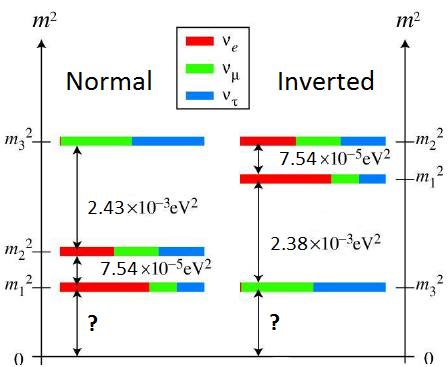
\includegraphics[width=.5\textwidth]{figures/hierarchy_alterred.png}
                \caption{The two possible hierarchies of neutrino masses.  The colors depict the mixing between the mass and flavor bases.}
\label{fig:numasshier}
\end{figure}

Neutrino oscillation demonstrates that neutrinos have non-zero mass, and though oscillation experiments measure the mass squared differences, the absolute masses of the three neutrinos remain unknown.  Cosmology can put limits on the sum of the three neutrino masses.  The Planck collaboration reports an upper bound on this sum at $\sum\limits_{i} m_{i} < 0.23$~eV \cite{Planck}.  The KATRIN experiment is expected to have a sensitivity of $m_{\bar{\nu}_{e}} < 0.2$~eV (90\% CL) for absolute neutrino mass from a careful measurement of tritium beta decay very near the Q-value (maximal decay energy) \cite{KATRIN}.

\section{Double Beta Decay}

Double beta decay is the simultaneous decay of two neutrons in a nucleus into two protons and two electrons.  Two-neutrino double beta decay ($2\nu\beta\beta$), shown in Fig. \ref{fig:feynman_diags}(left), is allowed by the Standard Model and has been observed in about a dozen isotopes with half-lives around $10^{19}$-$10^{21}$ years.  Similar to beta decay, an anti-neutrino accompanies each electron in this decay, broadening the spectrum of the summed electron energy. This is a second-order process, and very a rare, requiring low backgrounds to measure.

\begin{figure} %[H]
        %\centering
        %\begin{subfigure}
                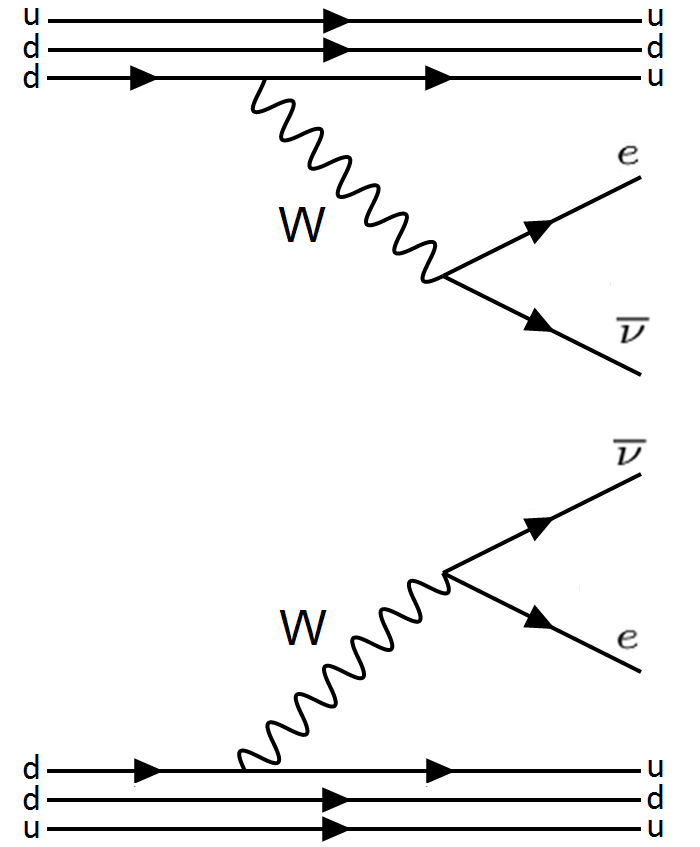
\includegraphics[width=.35\textwidth]{figures/feynman_2nu_quarks.png}
                %\caption{barf}
%        %\end{subfigure}
        %\begin{subfigure}
                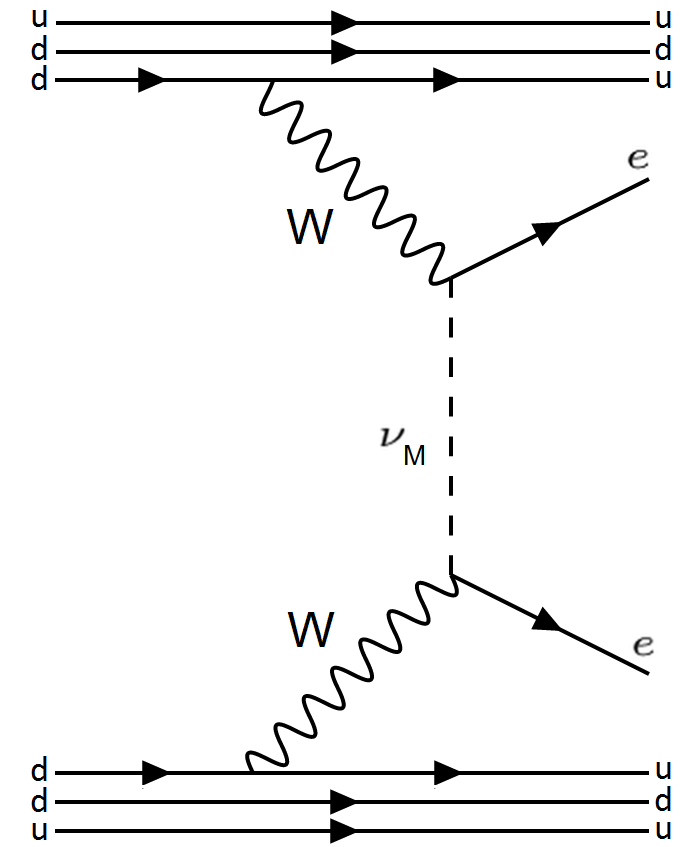
\includegraphics[width=.35\textwidth]{figures/feynman_0nu_quarks.png}
                \caption{Two-neutrino (left) and neutrinoless (right) double beta decay.}
        %\end{subfigure}
        \label{fig:feynman_diags}
\end{figure}

%\begin{table}[!htbp]
%\caption{$2\nu\beta\beta$ half-lives measured for various isotopes.} %not sure what [Small Table], between \caption and {}, w/ no spaces, does
%\label{table:bb_isotopes}
%\begin{tabular}{c|c|c}
%Isostope & $T^{2\nu}_{1/2} (10^{21}$~y) & Experiment\\
%\hline
%$^{136}$Xe & $2.165 \pm 0.016 \pm 0.059$ & EXO-200\\
%$^{76}$Ge & $1.84^{+0.14}_{-0.10}$ & GERDA\\
%\end{tabular}
%\end{table}

Neutrinoless double beta decay, shown in Fig. \ref{fig:feynman_diags}(right), is a postulated and yet unobserved mode of double beta decay. In this case, the neutrino is exchanged as a virtual particle (which would require that it is its own anti-particle, i.e. a Majorana particle), and there are no neutrinos in the final products. If discovered, neutrinos would be determined to be Majorana particles, and lepton number would be violated.  The measured $0\nu\beta\beta$ half-life would also aid in determining absolute neutrino mass according to Eq. \ref{eqn:rate_vs_mass}:

\begin{equation}
T_{1/2}^{0\nu} = (G^{0\nu}(Q,Z)|M^{0\nu}|^{2}\braket{m_{\nu}}^{2})^{-1}
\label{eqn:rate_vs_mass}
\end{equation}

\noindent
where $T_{1/2}^{0\nu}$ is the $0\nu\beta\beta$ half-life,  $G^{0\nu}$ is a known phase space factor, and $M^{0\nu}$ is a model-dependent nuclear matrix element.  $\braket{m_{\nu}}$ is the effective Majorana neutrino mass:

\begin{equation}
\braket{m_{\nu}} = \sum\limits_{i} U_{ei}^{2} m_{i}.
\label{eqn:effectivemass}
\end{equation}

\noindent
The terms $U_{ei}$ contain the measured mixing angles $\theta_{12}$ and $\theta_{13}$, as well as the unknown CP-violating phases $\delta$, $\alpha_1$, and $\alpha_2$.

The sum of the energies of the emitted electrons in double beta decay will serve as the distinction between the two-neutrino and zero-neutrino modes, shown in Fig. \ref{fig:spectrum_bb}. In the two-neutrino mode, the total decay energy is shared probabilistically between the electrons and the neutrinos (the nuclear recoil energy is negligible), resulting in a broad distribution in the summed electron energy. (Recall the similarly broad electron energy in single beta decay, which ultimately led to discovery of the neutrino involved.) But in the zero-neutrino mode, essentially all of the decay energy is carried away by the two electrons, resulting in effectively a single allowed value for the total electron energy -- a peak in the summed electron energy spectrum at the Q-value. 

\begin{figure} %[H]
        \centering
                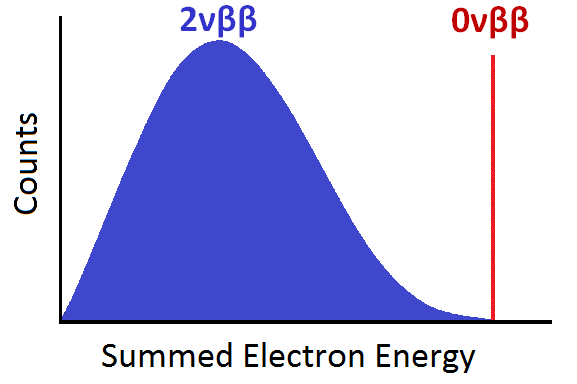
\includegraphics[width=.5\textwidth]{figures/spectrum_bb.png}
                \caption{Conceptual two-neutrino (blue) and zero-neutrino (red) double beta decay spectra.}
\label{fig:spectrum_bb}
\end{figure}

%  \emph{\color{red}make 0$\nu$ line shorter.}

The rarity of double beta decay requires very low backgrounds, especially around the Q-value for the $0\nu\beta\beta$ search. The next sections describe the experiments EXO-200 and its next-generation successor, nEXO, and how the barium tagging method studied in this work could be critical in obtaining essentially zero background in the second phase of nEXO operation.

\section{Enriched Xenon Observatory}

EXO-200 and nEXO (EXO standing for Enriched Xenon Observatory) are a progression of two experiments, each a liquid xenon (LXe) time projection chamber (TPC) designed to study the double beta decay of the isotope \textsuperscript{136}Xe, and ultimately to search for the zero-neutrino mode.  \textsuperscript{136}Xe is unique among the double beta decay isotopes in that it can be studied in a gas or liquid TPC instead of solid crystals or foils.  The 3D event position reconstruction abilities of a TPC have advantages in background reduction, as described in section \ref{subsec:EXO200}.  Purification of Xe is straightforward and can be done continuously in the detector.  LXe is transparent, and produces substantial ionization and scintillation at 178~nm when energy is deposited in the LXe \cite{EXO200TwoNuLong}.  A liquid TPC approach also offers the opportunity to identify, or ``tag'', the daughter \textsuperscript{136}Ba\textsuperscript{++} ion at the site of the double beta decay event, which would provide a method for background-free identification of $0\nu\beta\beta$ \cite{Moe1991}. Barium tagging is the focus of our group at CSU and is the subject of this thesis.  The following sections decribe the EXO-200 experiment, as well as nEXO, the next-generation tonne-scale LXe TPC, which is now in the research and development stage.  EXO-200 does not have barium tagging implemented, but it is hoped that nEXO will incorporate barium tagging in the second phase of operation. 

\subsection{EXO-200}
\label{subsec:EXO200}

%\newline

Located about half a mile underground in the Waste Isolation Pilot Plant (WIPP) near Carlsbad, NM, EXO-200 has been operational since 2011.  It is a TPC using LXe enriched to 80.672 $\pm$ 0.14\% \textsuperscript{136}Xe \cite{EXO200TwoNuLong}, with a fiducial volume corresponding to 66.20~kg of \textsuperscript{136}Xe. It is designed to probe Majorana neutrino masses down to around 100~meV \cite{EXO200instrumentationPart1}.  The WIPP mine is in a salt basin, which contains lower levels of Uranium and Thorium than rock in a typical mine.

\begin{figure} %[H]
	\centering
	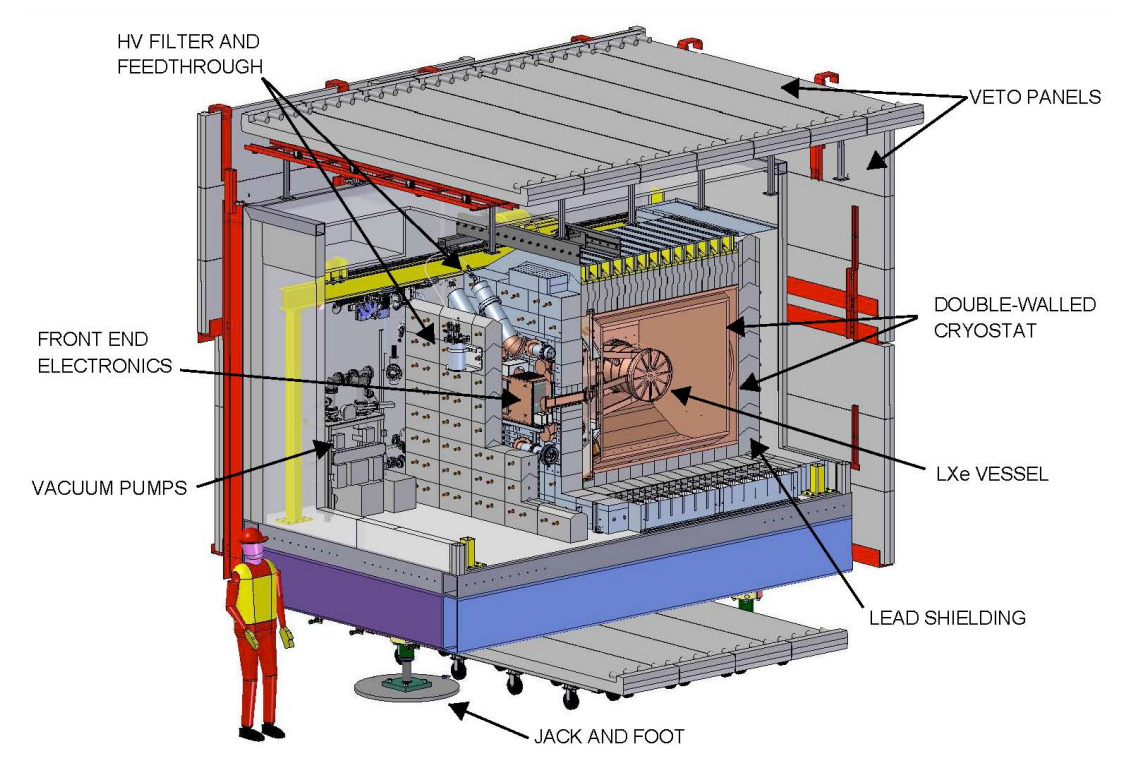
\includegraphics[width=.9\textwidth]{figures/cleanroom.png}
	\caption{Drawing of EXO-200 TPC Vessel with surrounding cryostat, lead walls, and muon veto panels.}
\label{fig:cleanroom}
\end{figure}

A schematic diagram of the TPC in the class 100 cleanroom is shown in Fig. \ref{fig:cleanroom}.  Several layers of lead wall surround the copper cryostat, which is filled with HFE-7000, a cryogenic fluid which keeps the TPC cooled to LXe temperatures  The HFE also provides shielding for the detector.  The TPC vessel is made of low-radioactivity copper, and is kept as thin as possible to minimize backgrounds.  Scintillating panels on the outside of the cleanroom provide a cosmic ray muon veto.

\begin{figure} %[H]
	\centering
	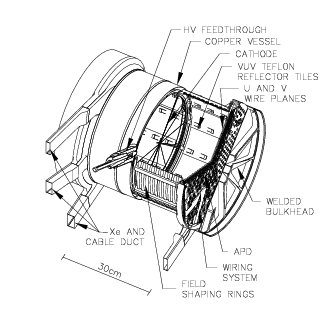
\includegraphics[width=.9\textwidth]{figures/TPC.png}
	\caption{EXO-200 TPC cutaway view \cite{EXO200TwoNuLong}.}
\label{fig:tpc}
\end{figure}

A cut-away view of the EXO-200 detector is shown in Fig. \ref{fig:tpc}.  It is two mirrored TPCs which share a cathode.  The detection planes are a combination of ionized charge induction/collection wires and large area avalanche photodiodes (LAAPDs), which detect scintillation light \cite{APDs}.

\begin{figure} %[H]
	\centering
	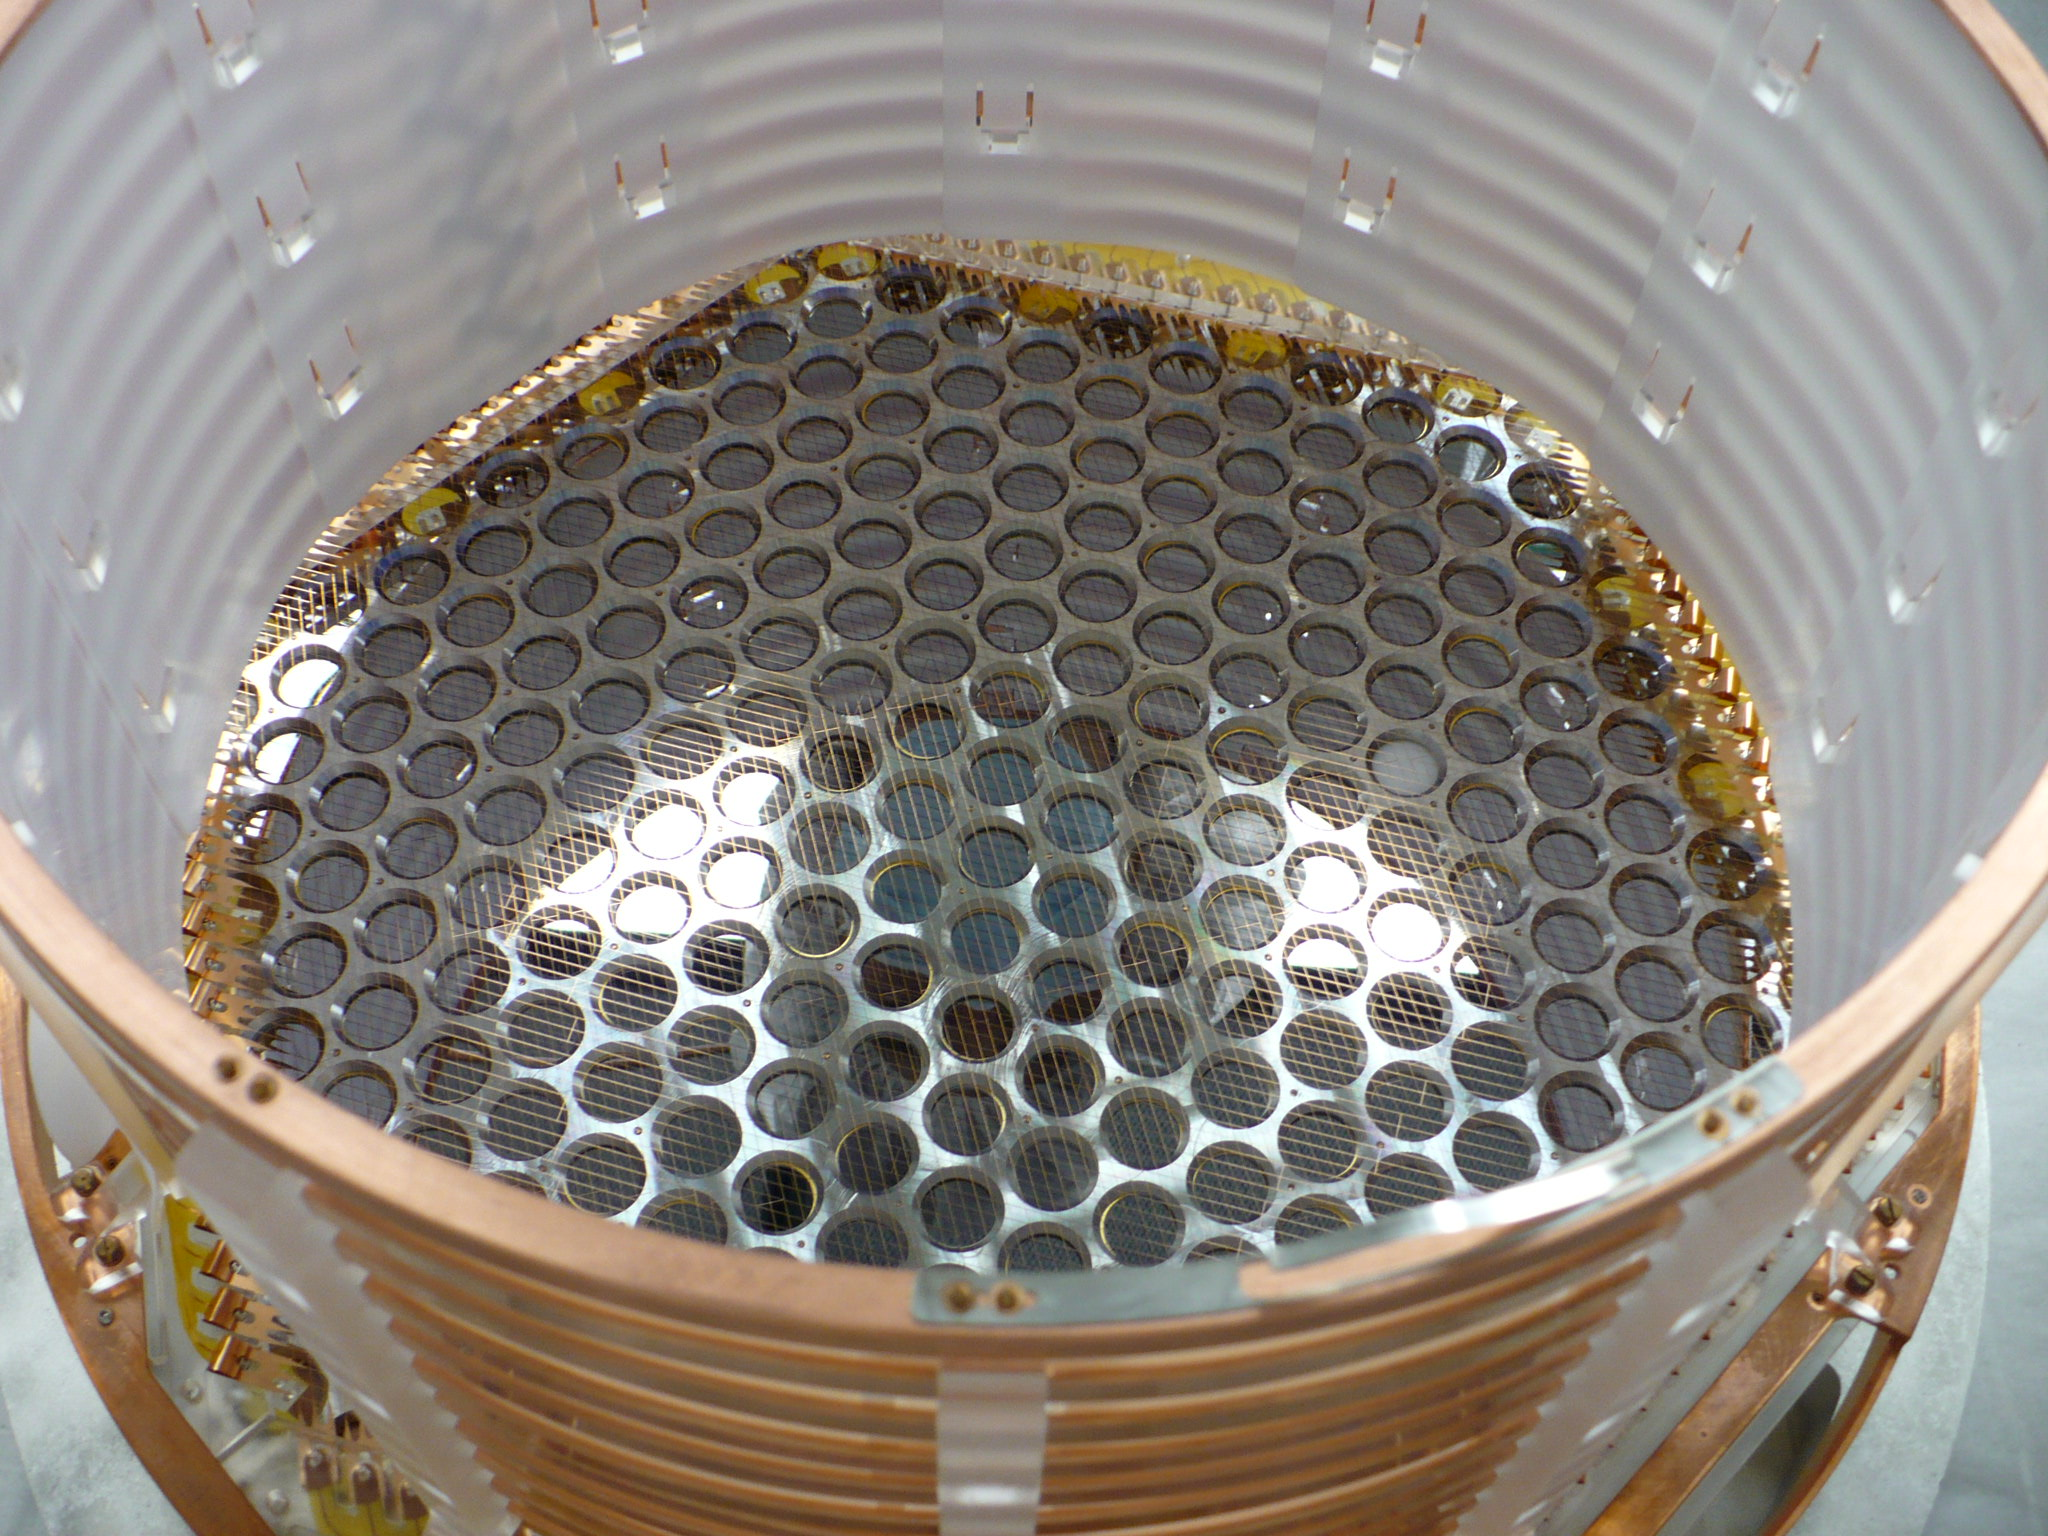
\includegraphics[width=.9\textwidth]{figures/TPCphoto.jpeg}
	\caption{View of the detection plane in one of the two EXO-200 TPCs.}
\label{fig:tpcphoto}
\end{figure}

A view into one of the TPCs is shown in Fig. \ref{fig:tpcphoto}.  On the detection plane, holes for the LAAPDs can be seen below the cross-hatched u- and v-wires.  The white material on the inner wall is the Teflon reflector.  When a double beta decay event occurs in the LXe, the energetic electrons ionize many surrounding Xe atoms, as well as produce a scintillation signal.  %Scintillation light provides an initial time for z-measurement of the event, as well as an energy measurement.

\begin{figure} %[H]
	\centering
	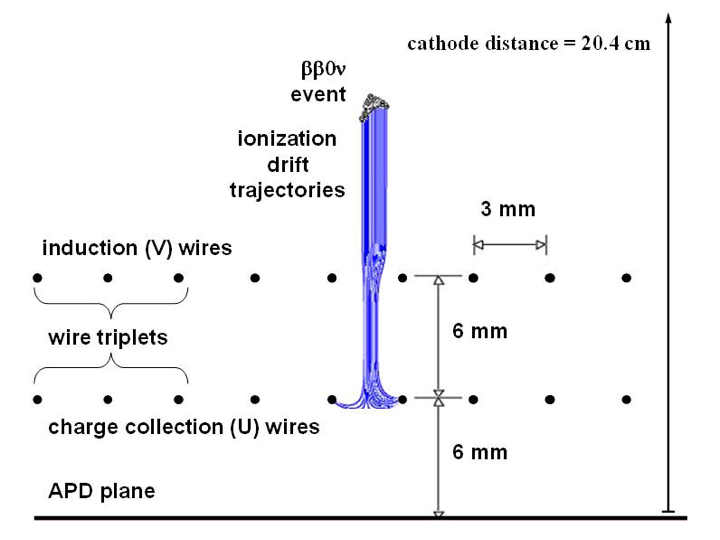
\includegraphics[width=.7\textwidth]{figures/anodecathodedriftcharges.png}
	\caption{EXO-200 event topology.  }
\label{fig:detectionplane}
\end{figure}

The cathode is set to -8~kV, providing an electric field of 374~V/cm across the 20~cm drift length of each TPC.  Ionized electrons drift from the decay site, first passing the v-wires, which receive an induction signal as depicted in Fig. \ref{fig:detectionplane}, and are then collected by the u-wires, which are set at a 60$^\circ$ angle from the v-wires.  An electric field of 778~V/cm between the u- and v-wires ensures 100\% v-wire transparency.  The charge collection provides an energy measurement.  Together, the u- and v-wires give an x/y position measurement for the event.  The time between the initial scintillation detection and the charge collection give a z position.  Thus a 3D position can be reconstructed for the event if u-wire, v-wire, and scintillation signals are detected.  \cite{EXO200TwoNuLong}  

\begin{figure} %[H]
	\centering
	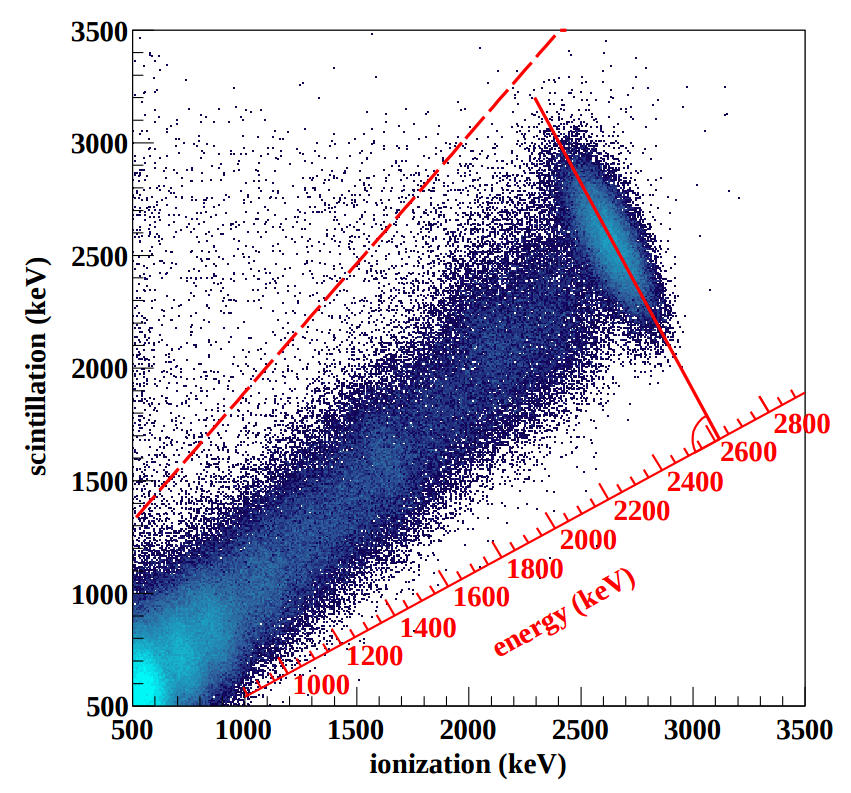
\includegraphics[width=.5\textwidth]{figures/anticorr.png}
	\caption{Anti-correlation between ionization and scintillation in events from the \textsuperscript{228}Th calibration source in EXO-200.  The dashed red line defines a cut on non-reconstructed events. \cite{EXO2000nuOriginal}}
\label{fig:antiCorr}
\end{figure}

The anti-correlation between ionization and scintillation signals of individual events in LXe \cite{anticorr} is exploited in EXO-200 to improve the energy resolution.  Energies measured by ionization and scintillation of events produced by the \textsuperscript{228}Th gamma source, one of the sources used to calibrate the EXO-200 detector, are plotted in Fig. \ref{fig:antiCorr}.  The tilt of the full absorption ellipse of the 2615~keV gamma line demonstrates the anti-correlation.  A ``rotated energy" is defined according to this tilt in order to optimize energy resolution.

%Energy resolution is important in a $0\nu\beta\beta$ search, as it distinguishes those events from $2\nu\beta\beta$ events in the tail of their spectrum.

Having a reconstructed 3D event position is important in several ways.  Firstly, position-based corrections to scintillation and charge collection can be applied.  For charge, electronegative impurities in the LXe will absorb the drifting charge, requiring a drift-length (z-position) correction.  High purity levels, measured in terms of electron lifetime, of 2-5ms and higher are maintained in EXO-200, resulting in a correction of a few \% for maximal drift lengths.  For scintillation, a 3D correction is applied, as some regions have more efficient light collection by the LAAPDs.  A 3D position also allows a fiducial volume to be defined.  A standoff distance from detector surfaces aids in distinction between gamma ray events and double beta decay events.  Gamma backgrounds, which mostly come from detector materials, exhibit some attenuation in the LXe.  Double beta decay events are uniformly distributed in the LXe.  Finally, 3D reconstruction allows the distinction between single-site (SS) and multi-site (MS) events.  A MS event is one where two spatially separated events occur in the same 2048-$\mu s$ time window.  These are mostly caused by gamma events, which can Compton-scatter one or more times in the LXe.  Rejecting MS events further aids in separating gamma events from double beta decay events.  \cite{EXO200TwoNuLong} Barium tagging will also benefit from a 3D reconstructed event position in nEXO.

%Calibration of EXO-200 is done using various radioactive sources which can be moved to several positions around the outside of the TPC.  Several different sources [\textsuperscript{137}Cs, \textsuperscript{60}Co, \textsuperscript{228}Th] span the energy range of interest, but the main source is $^{228}$Th, which produces gamma rays at [???]~MeV (\textsuperscript{208}Tl peak ... in chain right?), near the Q-value of $^{136}$Xe double beta decay where the $0\nu\beta\beta$ peak will be.  Source calibration data also provides a comparison between data and Monet-Carlo simulation, and provides the data for purity measurement and Light Map determination.  Data and Monte-Carlo for $^{228}$Th are shown in Fig. [ref fig source agreement].

\begin{figure} %[H]
	\centering
	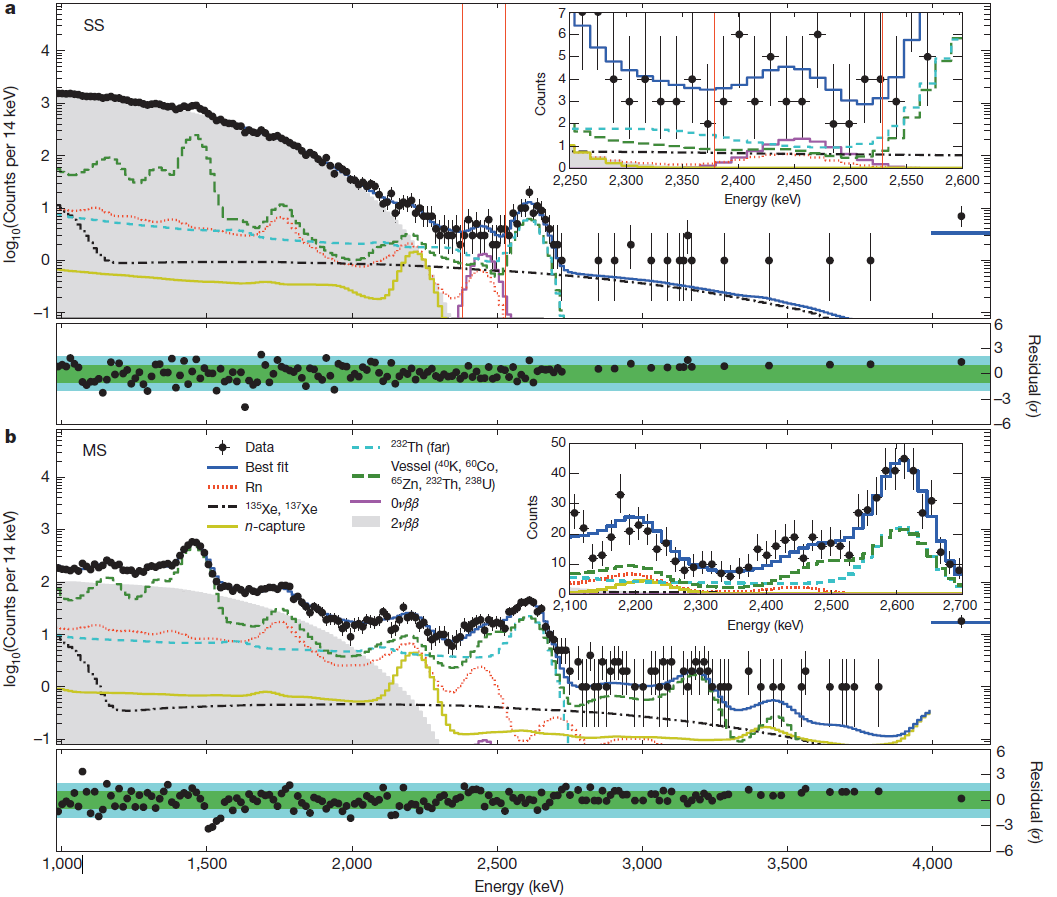
\includegraphics[width=.95\textwidth]{figures/0nu_spectrum_nature.png}
	\caption{EXO-200 energy spectrum of events from the latest $0\nu\beta\beta$ search analysis.  The insets show a zoom into the region of interest around the $2\nu\beta\beta$ end point. \cite{EXO2000nuNature}}
\label{fig:exo200data}
\end{figure}

The final data set is fit using a combination of probability distribution functions (PDFs) for $0\nu\beta\beta$, $2\nu\beta\beta$, and background components.  Fits to the final energy spectrum data for (a) SS events, and (b) MS events are shown in Fig. \ref{fig:exo200data} for the most recent $0\nu\beta\beta$ analysis.  The green bands beneath each plot show the residuals vs. energy.  The $2\nu\beta\beta$ spectrum, in gray, dominates the signal in the SS spectrum below the Q-value.  The vertical red lines in the SS spectrum outline the $\pm 2 \sigma$ region of interest around the Q-value, where the $0\nu\beta\beta$ peak will lie.  The insets are a zoom into this region.  The best fit value for $0\nu\beta\beta$ in this dataset is non-zero, but it is consistent with the null hypothesis at $1.2 \sigma$.  This sets an upper limit on the $0\nu\beta\beta$ half-life at $T^{0\nu\beta\beta}_{1/2} < 1.1 \times 10^{25}$~yr (90\% CL), which corresponds to $\braket{m_{\nu_{e}}} < $190-450~meV depending on nuclear matrix element calculations \cite{EXO2000nuNature}.  The $2\nu\beta\beta$ half-life has also been measured in EXO-200 as $T^{2\nu\beta\beta}_{1/2} = 2.165 \pm 0.016$(stat)$ \pm 0.059$(sys)$ \times 10^{21}$~yr \cite{EXO200TwoNuLong}.  This is the most precise $2\nu\beta\beta$ measurement to date and is consistent with previous measurements by EXO-200 in 2011 \cite{EXO200TwoNuOriginal} and KamLAND-ZEN in 2012 \cite{KamLAND}.

\subsection{nEXO}

The next-generation successor to EXO-200 is nEXO, a $\sim$5~ton LXe TPC which will probe Majorana neutrino masses down to the 10~meV scale.  A schematic diagram of the nEXO detector in the SNOLAB cryopit, one of the possible locations for nEXO, is shown in Fig. \ref{fig:nEXO_cryopit}.  Similar to EXO-200, the copper-housed TPC will be submerged in HFE fluid, inside a copper cryostat.  The cryostat will be insulated and submerged in a large volume of water shielding, in which photo-multiplier tubes will provide a muon veto by observing Cherenkov radiation.  nEXO will be a single TPC.  Rather than wires, nEXO will use tile electrodes for charge readout, shown in Fig. \ref{fig:nEXO_readout}.  Silicon photo-multipliers on the sides of the detector will be used for light detection.

\begin{figure} %[H]
	\centering
	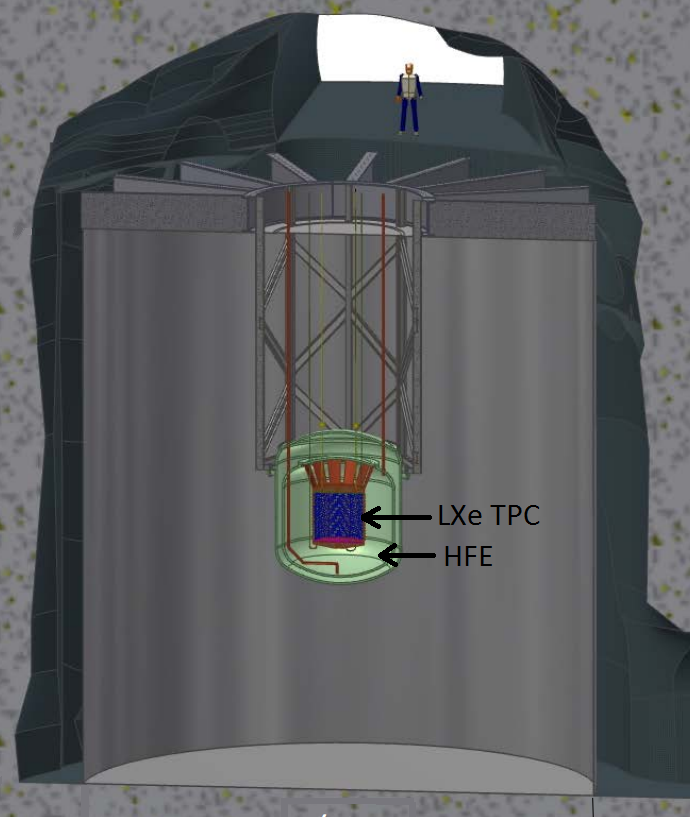
\includegraphics[width=.7\textwidth]{figures/nEXO_cryopit.png}
	\caption{nEXO TPC in the SNOLAB cryopit.}
\label{fig:nEXO_cryopit}
\end{figure}

\begin{figure} %[H]
	\centering
	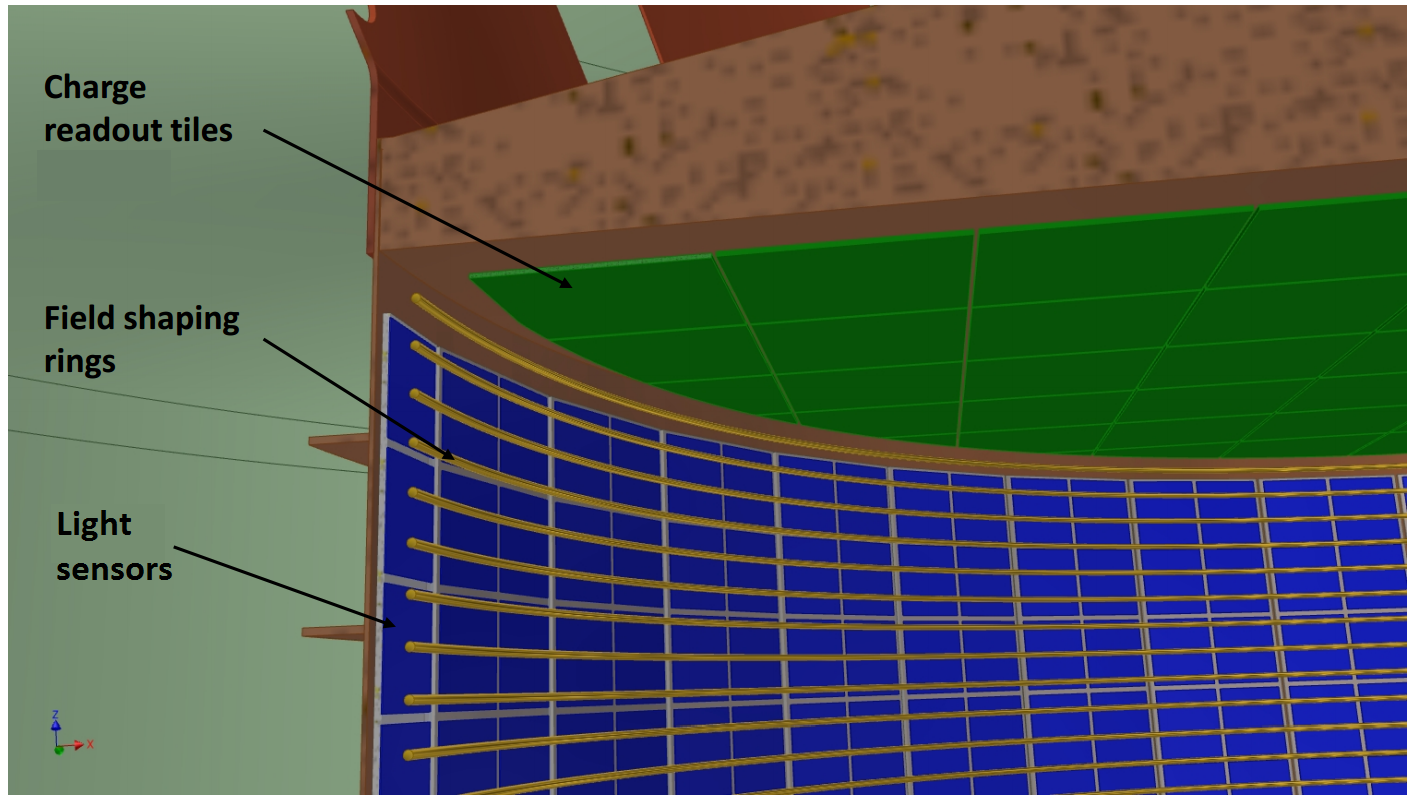
\includegraphics[width=.7\textwidth]{figures/nEXO_readout.png}
	\caption{nEXO readout.}
\label{fig:nEXO_readout}
\end{figure}

The sensitivity projections for nEXO are shown in Fig. \ref{fig:sensitivity_nEXO}, along with those of EXO-200.  EXO-200 probes the degenerate mass region down to about 0.1~eV.  nEXO will reach the non-degenerate region where the two possible mass hierarchies split, and will probe the full inverted hierarchy.  The addition of barium tagging would be a very significant advance, as it would push the mass sensitivity down into the region allowed only by the normal hierarchy.

% {\color{gray}[ref for this?]}

\begin{figure} %[H]
	\centering
	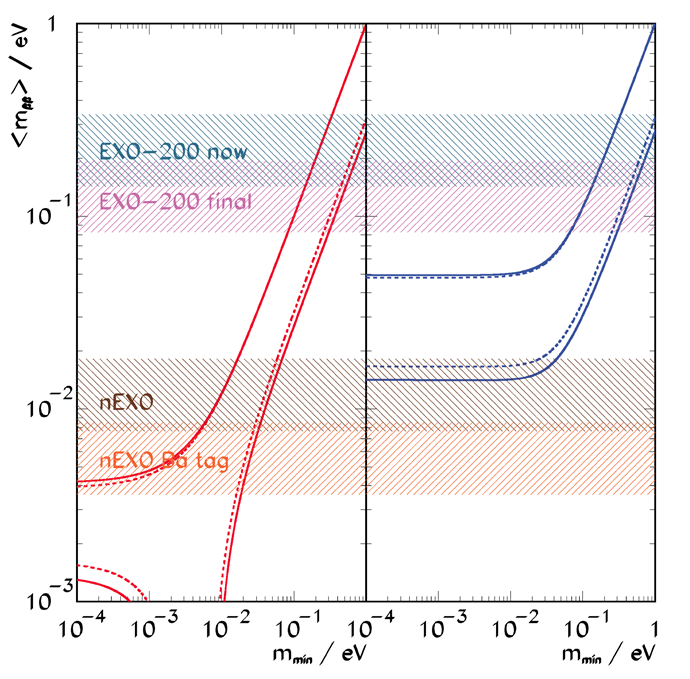
\includegraphics[width=.7\textwidth]{figures/sensitivity_v2.png}
	\caption{nEXO projected sensitivity to the effective Majorana neutrino mass vs. the minimum of the three masses neutrino m$_{min}$.  The dotted (solid) lines denote the 1(2)-$\sigma$ region allowed by neutrino oscillation measurements.}
\label{fig:sensitivity_nEXO}
\end{figure}

\subsection{Barium Tagging}

The ability to observe the daughter of each $0\nu\beta\beta$ event is the ultimate background rejection technique.  No background events generate a Ba daughter except $2\nu\beta\beta$ of \textsuperscript{136}Xe \cite{Moe1991}.  Several possible barium tagging techniques have been proposed for nEXO.  The original and most natural concept is to direct one or more lasers at the decay site to induce fluorescence of the barium daughter.  This technique was explored by our group, and has been abandoned for now because Ba\textsuperscript{+} fluorescence was not unambiguously identified in LXe \cite{Kendy}.

%Another concept was to grab the daughter in SXe on a cold probe, similar to the method explored in this thesis, but to then evaporate the SXe and drift the daughter into a trap for detection in vacuum.  This method was abandoned when extraction of barium from SXe samples could not be achieved by Liang Yang's group [ref?].

A few barium tagging techniques continue to be explored.  One of these is to grab the daughter on a probe surface, brought to the decay site by a probe.  It would then be moved to a location where it can be desorbed from that surface by an infrared laser, and subsequently resonantly ionized by two lasers in order to detect it by time-of-flight spectroscopy.  The apparatus for the study of this method is described in \cite{Twelker2014}, along with some initial results.

The other leading technique for barium tagging in LXe, now the focus of our group and the subject of this thesis, is barium tagging in solid xenon (SXe).  In this method, a cold probe would be inserted to the site of the candidate $0\nu\beta\beta$ event, and additional cooling would be applied to trap the Ba or Ba\textsuperscript{+} daughter in a small amount of SXe.  The single Ba/Ba\textsuperscript{+} would be observed by laser-induced fluorescence in the SXe, a technique more generally called matrix isolation spectroscopy.  A concept for a probe is shown in Fig. \ref{fig:probe}.  The SXe layer is formed on a sapphire window at the end of the probe.  Sapphire is a good candidate for a substrate because it has good thermal conductivity at low temperature and is highly transparent.  An excitation laser may be brought into the probe through a fiber, and scanned across the sapphire to excite the Ba/Ba\textsuperscript{+} in the SXe.  A return fiber could collect the laser reflection to measure the SXe thickness via interference fringes.  The Ba/Ba\textsuperscript{+} fluorescence would then be collected by a lens/filter system and imaged onto a CCD.  Additional components, not shown, would be required for cooling the sapphire, either by liquid He or by a Joule-Thompson nozzle.

\begin{figure} %[H]
	\centering
	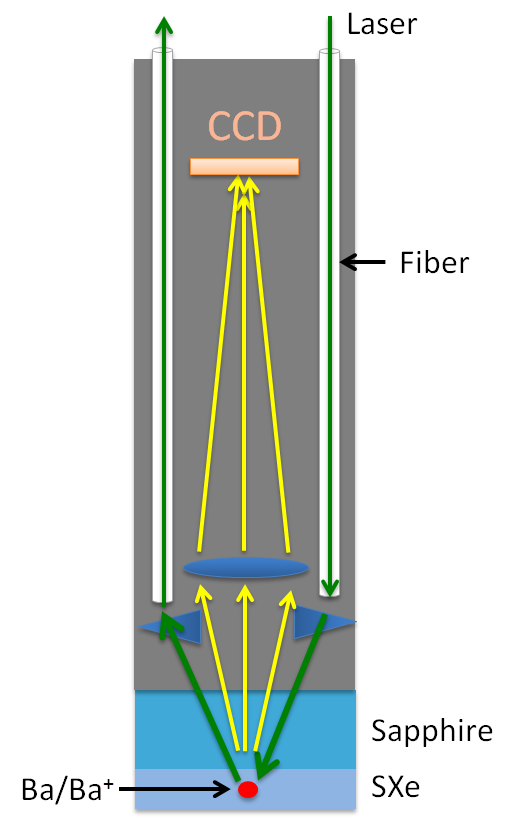
\includegraphics[width=.5\textwidth]{figures/probe_flat.png}
	\caption{Concept for a cryoprobe for \textsuperscript{136}Ba\textsuperscript{+} daughter ion capture and detection in SXe, and a concept for internal collection optics.}
\label{fig:probe}
\end{figure}

Whether the daughter Ba will neutralize or remain ionized in SXe is not yet known.  It is expected that a Ba\textsuperscript{++} daughter of $0\nu\beta\beta$ will neutralize rapidly to Ba\textsuperscript{+} by charge transfer in LXe, since the LXe conduction band gap is slightly less than the ionization potential for Ba\textsuperscript{+} \cite{Moe1991}.  Further neutralization by recombination with the electron cloud could also occur.  However, a study of neutralization of \textsuperscript{214}Bi daughters of \textsuperscript{214}Pb beta decay in EXO-200 has observed a high percentage, 76(5)\%, of ionized daughters, and negligible subsequent neutralization in many minutes \cite{alphaion}.  This provides an expectation of a high percentage of ionized \textsuperscript{136}Ba daughters of $0\nu\beta\beta$ in LXe in the singly ionized state.

%The next chapter describes theory relevant to single Ba/Ba\textsuperscript{+} detection in SXe matrices.
\chapter{Theory}
\label{chapter:theory}
%\label{chap:theory} this doesn't seem to work

Theory relevant to the spectroscopy of single Ba atoms and Ba\textsuperscript{+} ions in SXe matrices is discussed, beginning with the spectroscopy of Ba and Ba\textsuperscript{+} in vacuum in Sec. \ref{sec:vacuum}, with a numerical solution to a 5-level rate equations model in Sec. \ref{sec:model}.  Matrix isolation spectroscopy of metal species in solid noble gas matrices is discussed in Sec. \ref{sec:matrix}.  Finally, fluorescence efficiency and cross section calculations are presented in Sec. \ref{sec:fluorEff}.

\begin{table}[!htbp]
\caption{Transition rates for the lowest-lying energy levels of Ba and Ba\textsuperscript{+} in vacuum.} %not sure what [Small Table], between \caption and {}, w/ no spaces, does
\label{table:BaTransitions}
\begin{tabular}{c|c|c c}
& Transition & Rate ($s^{-1}$) &  \\
\hline
Ba & $6s6p$ $^{1}$P$_{1}$\textsuperscript{o} $\rightarrow 6s^{2}$ $^{1}$S$_{0}$ & $1.19 \times 10^{8}$ & \cite{BaAllowedTransitions} \\
& $6s6p$ $^{1}$P$_{1}$\textsuperscript{o} $\rightarrow 6s5d$ $^{1}$D$_{2}$ & $2.50 \times 10^{5}$ & \cite{BaAllowedTransitions} \\
& $6s6p$ $^{1}$P$_{1}$\textsuperscript{o} $\rightarrow 6s5d$ $^{3}$D$_{2}$ & $1.1 \times 10^{5}$ & \cite{BaAllowedTransitions} \\
& $6s6p$ $^{1}$P$_{1}$\textsuperscript{o} $\rightarrow 6s5d$ $^{3}$D$_{1}$ & $3.1 \times 10^{3}$ & \cite{BaAllowedTransitions} \\
& $6s5d$ $^{1}$D$_{2} \rightarrow 6s^{2}$ $^{1}$S$_{0}$ & $4$ & \cite{Ba1D2and3D1} \\
& $6s5d$ $^{3}$D$_{2} \rightarrow 6s^{2}$ $^{1}$S$_{0}$ & $1.45 \time 10^{-2}$ & \cite{Ba3D2} \\
& $6s5d$ $^{3}$D$_{1} \rightarrow 6s^{2}$ $^{1}$S$_{0}$ & $1.7 \time 10^{-2}$ & \cite{Ba1D2and3D1} \\
%& $6s6p$ $^{3}$P$_{1}$\textsuperscript{o} $\rightarrow 6s^{2}$ $^{1}$S$_{0}$ & {\color{red}???} & {\color{red}???}\\
\hline
Ba\textsuperscript{+} & $6p$ $^{2}P_{3/2}$\textsuperscript{o} $\rightarrow 6s $ $^{2}S_{1/2}$ & $1.11 \times 10^{8}$ & \cite{BaAllowedTransitions} \\
& $6p$ $^{2}P_{1/2}$\textsuperscript{o} $\rightarrow 6s$ $^{2}S_{1/2}$ & $9.53 \times 10^{7}$ & \cite{BaAllowedTransitions} \\
& $6p$ $^{2}P_{3/2}$\textsuperscript{o} $\rightarrow 5d$ $^{2}D_{5/2}$ & $4.12 \times 10^{7}$ & \cite{BaAllowedTransitions} \\
& $6p$ $^{2}P_{3/2}$\textsuperscript{o} $\rightarrow 5d$ $^{2}D_{3/2}$ & $6.00 \times 10^{6}$ & \cite{BaAllowedTransitions} \\
& $6p$ $^{2}P_{1/2}$\textsuperscript{o} $\rightarrow 5d$ $^{2}D_{3/2}$ & $3.10 \times 10^{7}$ & \cite{BaAllowedTransitions} \\
& $5d$ $^{2}D_{5/2} \rightarrow 6s$ $^{2}S_{1/2}$ & $3.8 \times 10^{-2}$ & \cite{BaPlusD52} \\
& $5d$ $^{2}D_{3/2} \rightarrow 6s$ $^{2}S_{1/2}$ & $1.3 \times 10^{-2}$ & \cite{BaPlusD32} \\
\end{tabular}
\end{table}

\section{Ba/Ba\textsuperscript{+} Spectroscopy in Vacuum}
\label{sec:vacuum}

Some of the low-lying energy levels for Ba in vacuum are shown in Fig. \ref{fig:elevsBa}.  Transition rates for the lowest-lying Ba energy levels in vacuum are shown in Table \ref{table:BaTransitions}.  The main transition is between the ground $6s^{2}$ $^{1}$S$_{0}$ state to the excited $6s6p$ $^{1}$P$_{1}$\textsuperscript{o} state.  Decays from the $^{1}$P$_{1}$\textsuperscript{o} state to three metastable D states have a branching ratio of about 1 in 330 excitations.  Decays back to ground from the D states are parity-forbidden, resulting in very low decay rates of around 4~s$^{-1}$ for the $^{1}$D$_{2}$ state, and around 0.01~s$^{-1}$ for the $^{3}$D states.  This can lead to significant optical pumping of these states during multiple cycles of excitation of the  $^{1}$S$_{0} \rightarrow ^{1}$P$_{1}$\textsuperscript{o} transition.

%, including that of $^{3}$P$_{1}$\textsuperscript{o} to ground.  Though decays into the $^{3}$P states from $^{1}$P$_{1}$\textsuperscript{o} are parity-forbidden, they may occur for Ba in a SXe matrix, in which case $^{3}$P$_{1}$\textsuperscript{o} to ground is relevant

\begin{figure} %[H]
	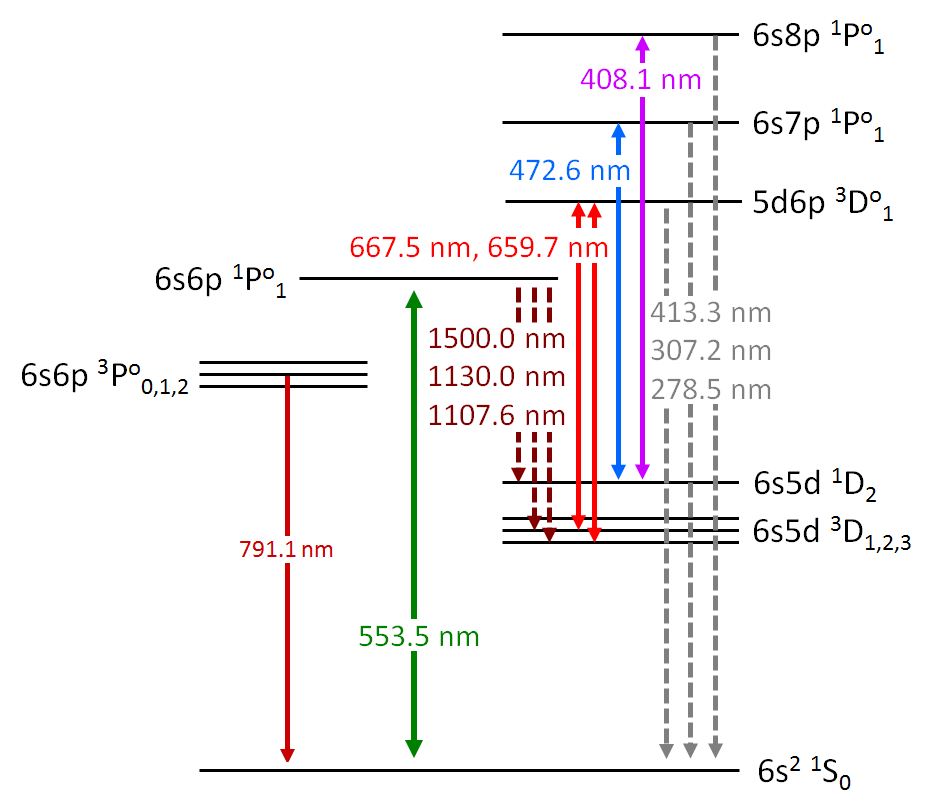
\includegraphics[width=.8\textwidth]{figures/elevs_Ba_extra_with3P1.png}
	\caption{Ba energy levels in vacuum.}
    \label{fig:elevsBa}
\end{figure}

The low-lying energy levels of Ba\textsuperscript{+} in vacuum are shown in Fig. \ref{fig:elevsBaPlus}.  Two strong transitions exist between the ground $6s$ $^{2}$S$_{1/2}$ state and the $6p$ $^{2}$P$_{1/2}$ and $6p$ $^{2}$P$_{3/2}$ excited states.  Branching ratios to the two metastable $^{2}$D states result in a decay into a $^{2}$D state after about 4 excitations.  Decay out of the $^{2}$D states takes tens of seconds.  Transition rates between these levels are listed in Table \ref{table:BaTransitions}.    

\begin{figure} %[H]
	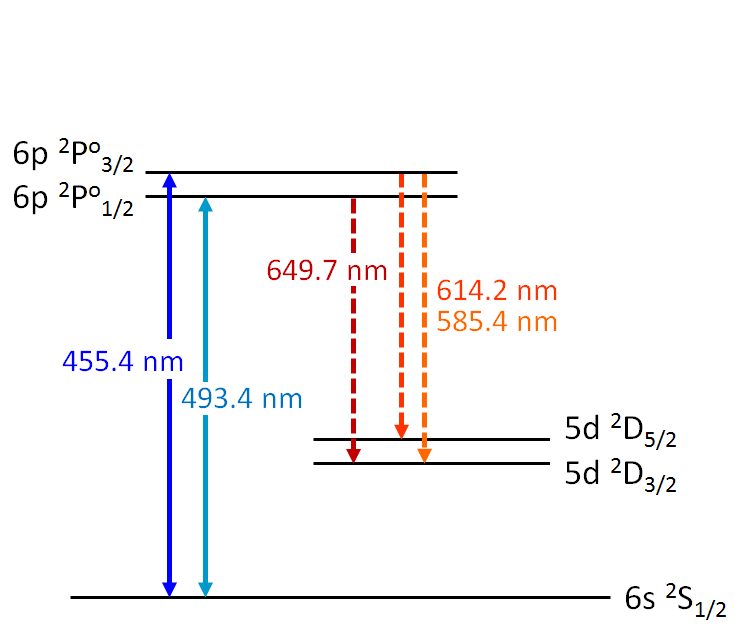
\includegraphics[width=.6\textwidth]{figures/elevs_Ba+_separate.png}
	\caption{Ba\textsuperscript{+} energy levels in vacuum.}
    \label{fig:elevsBaPlus}
\end{figure}

%These rates are shown in  along with each of the allowed transitions in Fig. \ref{fig:elevs}.

%The lowest-lying energy levels in vacuum for Ba and Ba\textsuperscript{+} are shown in Fig. \ref{fig:elevs}.  For Ba, the main transition is between the ground $6s^{2}$ $^{1}$S$_{0}$ to the excited $6s6p$ $^{1}$P$_{1}$\textsuperscript{o} state, however branching ratios from the P state result in a decay to one of three metastable D states in about 1 in 330 excitations.  For Ba\textsuperscript{+}, two strong transitions exist between the ground $6s$ $^{2}$S$_{1/2}$ and the $6p$ $^{2}$P$_{1/2}$ and $6p$ $^{2}$P$_{3/2}$ excited states.  Transitions to the two metastable D states are higher than for the atom, resulting in a decay into a D state after about 4 excitations.  These D states are metastable because they are parity-forbidden to decay back to the ground state, resulting in much lower decay rates.  These rates are shown in Table \ref{table:BaTransitions} along with each of the allowed transitions in Fig. \ref{fig:elevs}.

%\begin{figure}[H]
%	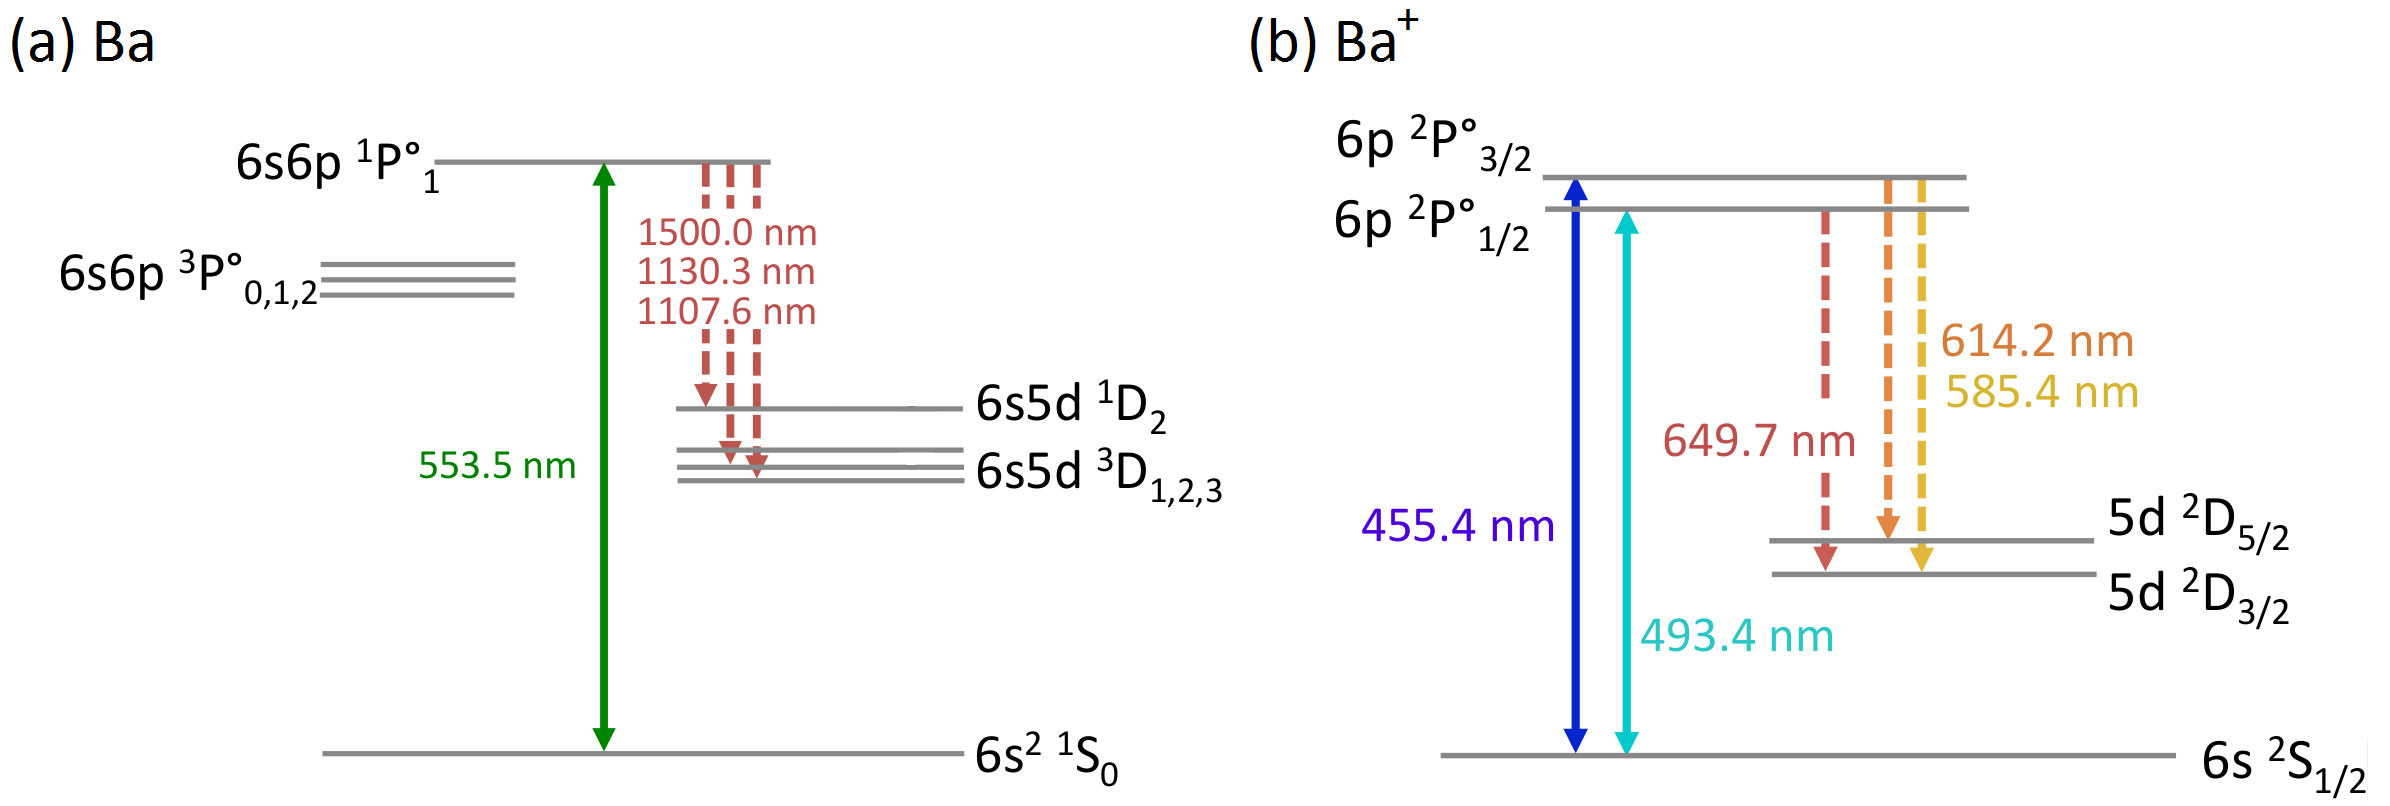
\includegraphics[width=.9\textwidth]{figures/elevs.png}
%	\caption{Energy level diagrams for (a) Ba and (b) Ba\textsuperscript{+}.}
%    \label{fig:elevs}
%\end{figure}

%These energy levels and their transition rates are well known, and are documented in the NIST Atomic Spectra Database.

Single atom/ion detection by fluorescence requires many excitation/emission cycles in order to detect an observable number of photons from a single atom/ion.  For Ba and Ba\textsuperscript{+}, in addition to the main excitation laser, lasers may be needed to depopulate the metastable D states once the atom/ion becomes optically pumped into one of them.  This recovery is called re-pumping.  For Ba atoms in vacuum, re-pumping can be accomplished via three infrared lasers at wavelengths 1107.6~nm, 1130.0~nm, and 1500.0~nm for the direct transitions back to the $6s6p$ $^{1}$P$_{1}$\textsuperscript{o} state.  An alternative re-pumping scheme is via excitation to higher-level states which have paths back to the ground state or the $6s6p$ $^{1}$P$_{1}$\textsuperscript{o} state.  A few such higher-level re-pump transitions are shown in Fig. \ref{fig:elevsBa}, including two red transitions to the $5d6p$ $^{3}$D$_{1}$\textsuperscript{o} state, and blue and violet transitions to the $6s7p$ $^{1}$P$_{1}$\textsuperscript{o} and $6s8p$ $^{1}$P$_{1}$\textsuperscript{o} states.  Trapping and detection of Ba atoms in vacuum in a magneto-optical trap (MOT) was achieved in \cite{BaMOT}.  This was done with two separate re-pumping schemes:  by incorporating three infrared re-pump transitions, as well as two infrared re-pump transitions and a 659.7-nm laser re-pumping the $6s5d$ $^{3}$D$_{1}$ state via the $5d6p$ $^{3}$D$_{1}$\textsuperscript{o} state.  Observation of trapped single Ba\textsuperscript{+} ions in vacuum has been achieved using 493.4~nm along with one re-pump laser at 649.7~nm \cite{BaPlus1978,singleBaPlusEXO}.

%, replacing the 1130.6-nm transition directly to $6s6p$ $^{1}$P$_{1}$\textsuperscript{o}

\section{5-level Rate Equations Model}
\label{sec:model}

A 5-level rate equations model for Ba transitions in vacuum, with excitation to the $6s6p$ $^{1}$P$_{1}$\textsuperscript{o} state, is shown schematically in Fig. \ref{fig:5lev}.  States 1 and 2 represent the $6s^{2}$ $^{1}$S$_{0}$ and $6s6p$ $^{1}$P$_{1}$\textsuperscript{o} states, respectively, and states 3, 4 and 5 represent the $6s5d$ $^{1}$D$_{2}$, $6s5d$ $^{3}$D$_{2}$, and $6s5d$ $^{3}$D$_{1}$ states, respectively.  The rate equations for this system, neglecting stimulated emission, are given in Eq. \ref{eqn:rateEqn}:


\begin{figure} %[H]
        \centering
                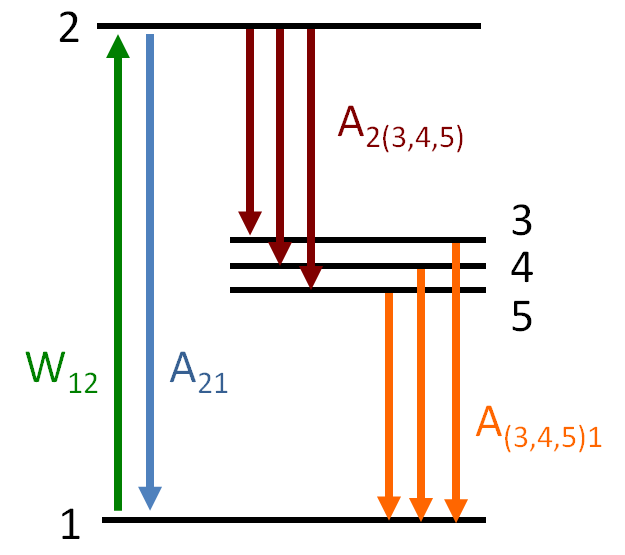
\includegraphics[width=.4\textwidth]{figures/5-level_general.png}
                \caption{5-level system diagram with excitation rate $W_{12}$ and decay rates $A_{ij}$.}
\label{fig:5lev}
\end{figure}

% is stated in Eqn. \ref{eqn:rateEqn}:

\begin{equation}
\begin{aligned}
\frac{dN_1}{dt} &= - W_{12}N_{1} + A_{21}N_{2} + A_{31}N_{3} + A_{41}N_{4} + A_{51} N_{5} \\
\frac{dN_2}{dt} &= W_{12}N_{1} - N_{2}(A_{21} + A_{23} + A_{24} + A_{25}) \\
\frac{dN_3}{dt} &= A_{23}N_{2} - A_{31}N_{3} \\
\frac{dN_4}{dt} &= A_{24}N_{2} - A_{41}N_{4} \\
\frac{dN_5}{dt} &= A_{25}N_{2} - A_{51}N_{5} \\
\end{aligned}
\label{eqn:rateEqn}
\end{equation}

\noindent
where $N_{i}$ is the population in state $i$, $A_{ij}$ is the spontaneous decay rate from state $i$ to state $j$, and $W_{12}$ is the excitation rate:

\begin{equation}
W_{12} =  \frac{\sigma I}{h \nu}
\label{eqn:w12}
\end{equation}

\noindent
where $\sigma$ is the cross section for excitation, $I$ is the laser intensity, and $h \nu$ is the excitation photon energy.

Under some experimental conditions, the assumption can be made that $W_{12}$ is small compared to the rates out of the $^{1}$P$_{1}$\textsuperscript{o} state.  In this case the population in the excited state $N_{2}$ is small compared to the populations of the other states.  Except for very short times, $dN_2/dt$ is also small compared to $W_{12} N_1$ and $N_2 A_{21}$.  For these conditions, there is an effective pumping rate for the D states:

\begin{equation}
W_{1i} = W_{12}\frac{A_{2i}}{A_{21} + A_{23} + A_{24} + A_{25}}
\label{eqn:smallW12pumpingRates}
\end{equation}

\noindent
where $i = 3,4,5$.  The fraction in Eq. \ref{eqn:smallW12pumpingRates} is the respective branching ratio from the excited state 2.  With this definition, the rate equations for states 3, 4, and 5 can be re-written as:

%, including the pumping rate back to ground

\begin{equation}
\begin{aligned}
\frac{dN_3}{dt} &= W_{13}N_{1} - A_{31}N_{3} \\
\frac{dN_4}{dt} &= W_{14}N_{1} - A_{41}N_{4} \\
\frac{dN_5}{dt} &= W_{15}N_{1} - A_{51}N_{5} \\
\end{aligned}
\label{eqn:smallW12populationRates}
\end{equation}

\noindent
where $N_{1} = 1 - N_{3} - N_{4} - N_{5}$ by conservation of total population.

For a numerical solution of these equations, initially all population is in the ground state ($N_{3} = N_{4} = N_{5} = 0$).  The model calculates the state populations $N_{i}$ at the end of each iterative time step, $t_{\text{step}}$, as:

\begin{equation}
\begin{aligned}
N_{i} = N_{i, previous} + \frac{dN_i}{dt}t_{\text{step}} \\
\end{aligned}
\label{eqn:smallW12populations}
\end{equation}

\noindent
where $i = 3,4,5$, and $dN_i/dt$ is determined at the beginning of each time step according to Eq. \ref{eqn:smallW12populationRates}.  Time steps of $t_{\text{step}} = 1~\mu$s were used.  In order to model data, which is taken in exposure time ($t_{\text{exp}}$) frames, the model iterates through $t_{\text{exp}}/t_{\text{step}}$ steps in each frame, accumulating fluorescence photons emitted at each step ($\Delta S_{\text{step}}$) according to the fluorescence rate times $t_{\text{step}}$:

\begin{equation}
\begin{aligned}
\Delta S_{\text{step}} = W_{12}  N_{1} \frac{A_{21}}{A_{21} + A_{23} + A_{24} + A_{25}}t_{\text{step}} \\
\end{aligned}
\label{eqn:smallW12counts}
\end{equation}

\noindent
To incorporate camera readout time, where laser exposure continues but fluorescence is not observed, populations and derivatives are iterated without adding to total counts.

\begin{figure} %[H]
        \centering
                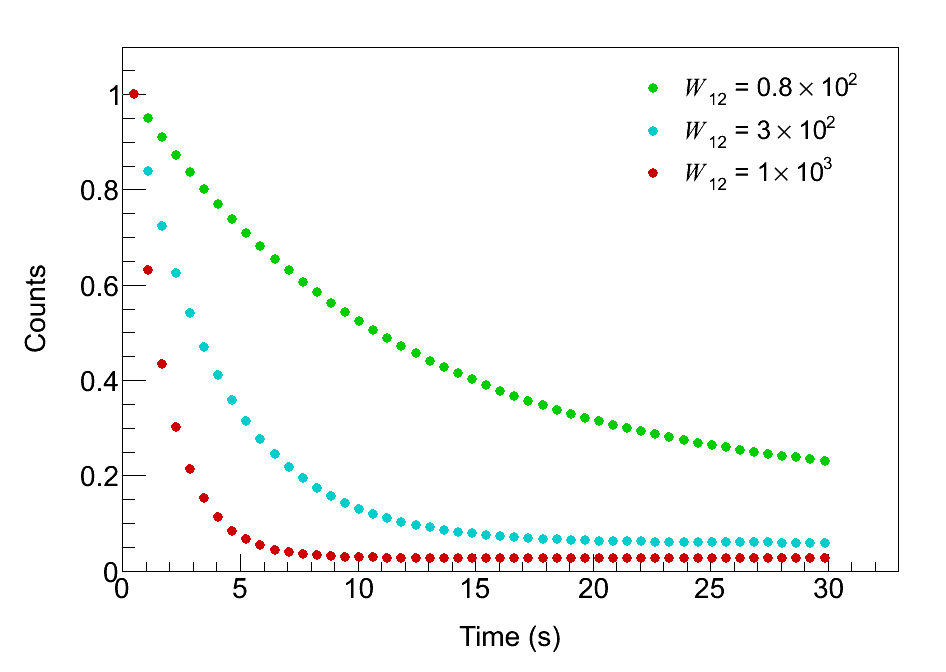
\includegraphics[width=.7\textwidth]{figures/thesis_modelExamples.png}
                \caption{Modeled photons emitted in 0.5-s exposure frames for three values of $W_{12}$, using vacuum Ba transition rates, normalized to the first point.  A readout time of 0.1~s is used between frames. }
\label{fig:modelExample}
\end{figure}

Examples of modeled normalized photons emitted vs. time are shown in Fig. \ref{fig:modelExample} for three values of $W_{12}$, using the transition rates of Ba in vacuum from Table \ref{table:BaTransitions}.  Decay of fluorescence occurs as atoms are optically pumped into the metastable D states.  For long times the curves reach a steady state value.  This model is compared to bleaching data of Ba in SXe in Sec. \ref{sec:bleach577and591}.

%\begin{equation}
%\begin{aligned}
%\frac{dN_1}{dt} &= - w_{12}N_{1} + a_{21}N_{2} + a_{31}N_{3} %+ a_{41}N_{4} + a_{51} N_{5} + a_{61}N_{6} \\
%\frac{dN_2}{dt} &= w_{12}N_{1} - N_{2}(a_{21} + a_{23} + %a_{24} + a_{25} + a_{26}) \\
%\frac{dN_3}{dt} &= a_{23}N_{2} - a_{31}N_{3} \\
%\frac{dN_4}{dt} &= a_{24}N_{2} - a_{41}N_{4} \\
%\frac{dN_5}{dt} &= a_{25}N_{2} - a_{51}N_{5} \\
%\frac{dN_6}{dt} &= a_{26}N_{2} - a_{61}N_{6}
%\end{aligned}
%\label{eqn:rateEqn}
%\end{equation}

\section{Matrix Isolation Spectroscopy}
\label{sec:matrix}

%\emph{\color{gray}May be good matrix isolation theory references in Ba Spec... yeah, 1 and 2 i think ... shon's 55, 57, 58 are probably good too and maybe overlapping}

In the matrix isolation technique, a species of interest is trapped in a crystal, or ``matrix," of inert atoms/molecules such that it can be studied at leisure.  To be effective, the temperature must be low enough to prevent diffusion of guest atoms, and the guest concentration must be low enough to prevent guest-guest interaction.  The technique was originally proposed and demonstrated in \cite{matrixIso}, where otherwise short-lived species in were studied by isolating them in various solid matrices.  The proposed method of Ba tagging in SXe is a unique application of matrix isolation spectroscopy.  In order to understand the spectroscopic effects which may be encountered due to interaction between the guest Ba atoms and Ba\textsuperscript{+} ions and the host Xe atoms, some effects encountered in systems of metal atoms in rare-gas matrices are discussed.

%Low concentrations of the guest species, ideally at least 1:$10^{3}$ host:guest ratio, prevent guest-guest interactions.  

\begin{figure} %[H]
        \centering
                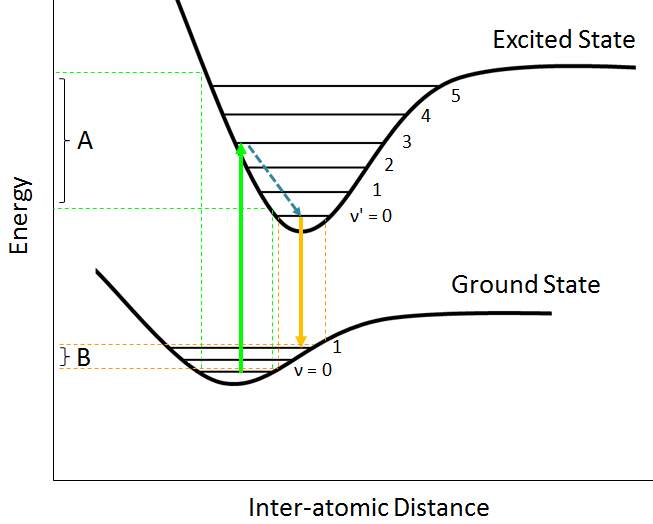
\includegraphics[width=.6\textwidth]{figures/FranckCondon3.png}
                \caption{Illustration of the Franck-Condon Principle resulting in red-shifted emission as well as broadening in absorption (A) and emission (B) due to vibrational modes $\nu$ ($\nu$') in the ground (excited) state.}
\label{fig:FranckCondon}
\end{figure}

The leading interaction between a guest atom and the host noble gas atoms is an induced dipole-dipole Van der Waals force.  For a metal atom of group I or II, this interaction is quite different when the atom is in the excited P state vs. the ground S state, resulting in general in different shaped potential energy curves \cite{crepin}.  To illustrate the concept, guesses at the ground and excited state potentials for a BaXe molecule are shown in Fig. \ref{fig:FranckCondon}.  In a cold matrix, the system will be mainly in the ground lattice vibrational state ($\nu =0$) before excitation.  According to the Franck-Condon principle, the strongest electronic excitation will occur to vibrational states whose wavefunctions overlap that of the ground state.  Because this occurs for a band of vibrations, the absorption is broadened.  The peak absorption energy is determined by the difference in potential energy between the ground state and the median vibrational state excited, which in general is not the same as the absorption energy of atoms in vacuum.  In the excited state, rapid decay occurs to the lowest vibrational state, and then a similar broadening in the spontaneous emission energy occurs.  A redshift in the emission is observed relative to the excitation.  Additionally, splitting of orbital degeneracy in the P state can produce triplet structures in the absorption according to the Jahn-Teller effect \cite{jahnteller}.  These features depend on the specific configuration of atoms surrounding the guest, and thus different spectra can be observed from guest atoms occupying different matrix ``sites."  Annealing a matrix after deposition can reveal the relative stability of various matrix sites \cite{crepin}.

%The ground S state of a group I or II atom is spherically symmetric, and being slightly larger in Van der Waals radius than Xe, it is likely to take the place of one or more Xe atoms in the fcc crystal (substitution), vs. existing in between Xe atoms in the crystal structure (interstitial).

%dynamic

%the strength of the Ba-Xe interaction, an induced dipole-dipole Van der Waals force, is quite different when the Ba is in the non-spherically-symmetric excited P state \cite{crepin}.  

% before electronic decay can occur

\begin{figure} %[H]
        \centering
                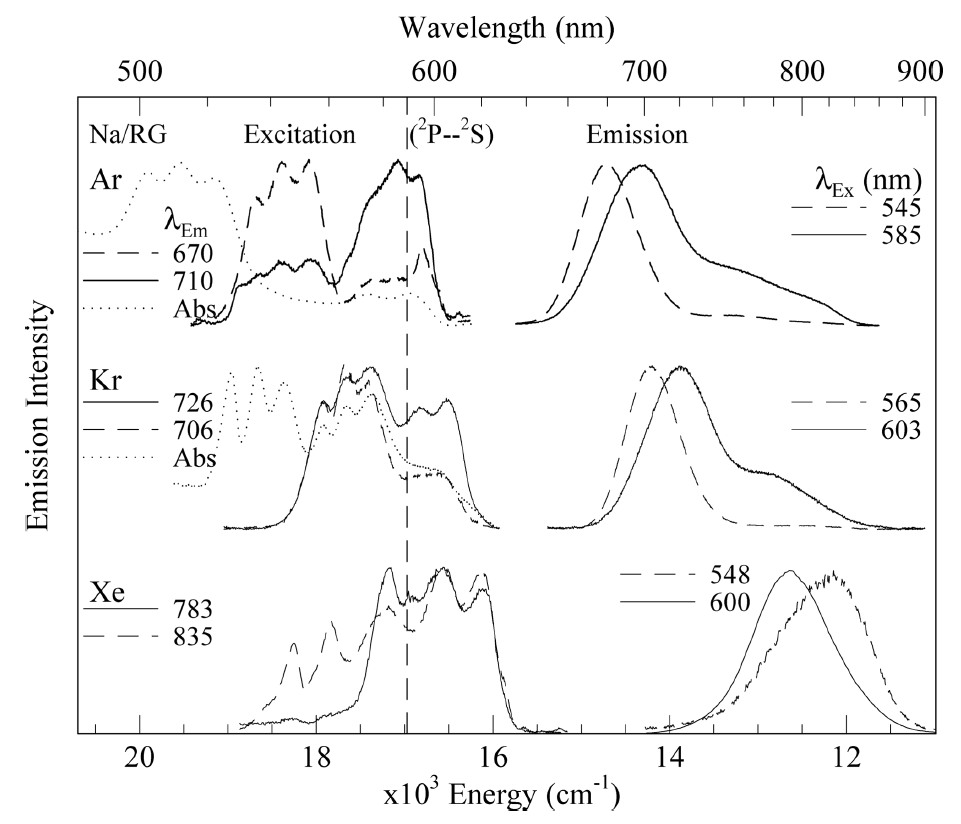
\includegraphics[width=.7\textwidth]{figures/Na_in_matrices.png}
                \caption{Excitation and emission spectra of Na atoms in SAr, SKr, and SXe.  \cite{matrixNa}}
\label{fig:matrixNa}
\end{figure}

As an example, the spectroscopy on Na atoms in solid rare-gas matrices was studied in \cite{matrixNa}.  Spectral features are exemplified in Fig. \ref{fig:matrixNa} for Na atoms in SAr, SKr, and SXe.  Excitation and emission are broadened to tens of nm.  Two or three different matrix sites are observed in the three matrices, with the largest red-shift in emission observed in SXe.  The triplet structures in excitation spectra are attributed to the Jahn-Teller effect.  The specific matrix configuration associated with each excitation triplet is identified in this paper through theoretical modeling of the Na-matrix interactions.

%As as example \emph{\color{gray}is there a more modern example paper you can use?}, the spectroscopy of Ba in solid Ar (SAr) and solid Kr (SKr) matrices was studied in \cite{SAr}.  The example of Ba in SAr is shown in Fig. \ref{fig:BaSAr}.  The absorption is 10s of nm broad with a multi-peak structure, and the emission is broadened to nms and red-shifted.  These were attributed to the main $6s^{2}$ $^{1}$S$_{0} \rightarrow 6s6p$ $^{1}$P$_{1}$\textsuperscript{o} transition and its spontaneous emission. \emph{\color{gray}talk about other aspects.....brian says the triplet is caused by P state degeneracy being split, but I don't see how this makes sense, and also I have the impression that there are multiple explanations like Jahn Teller -- you should have a feel for this....}

%\begin{figure} %[H]
%        \centering
%                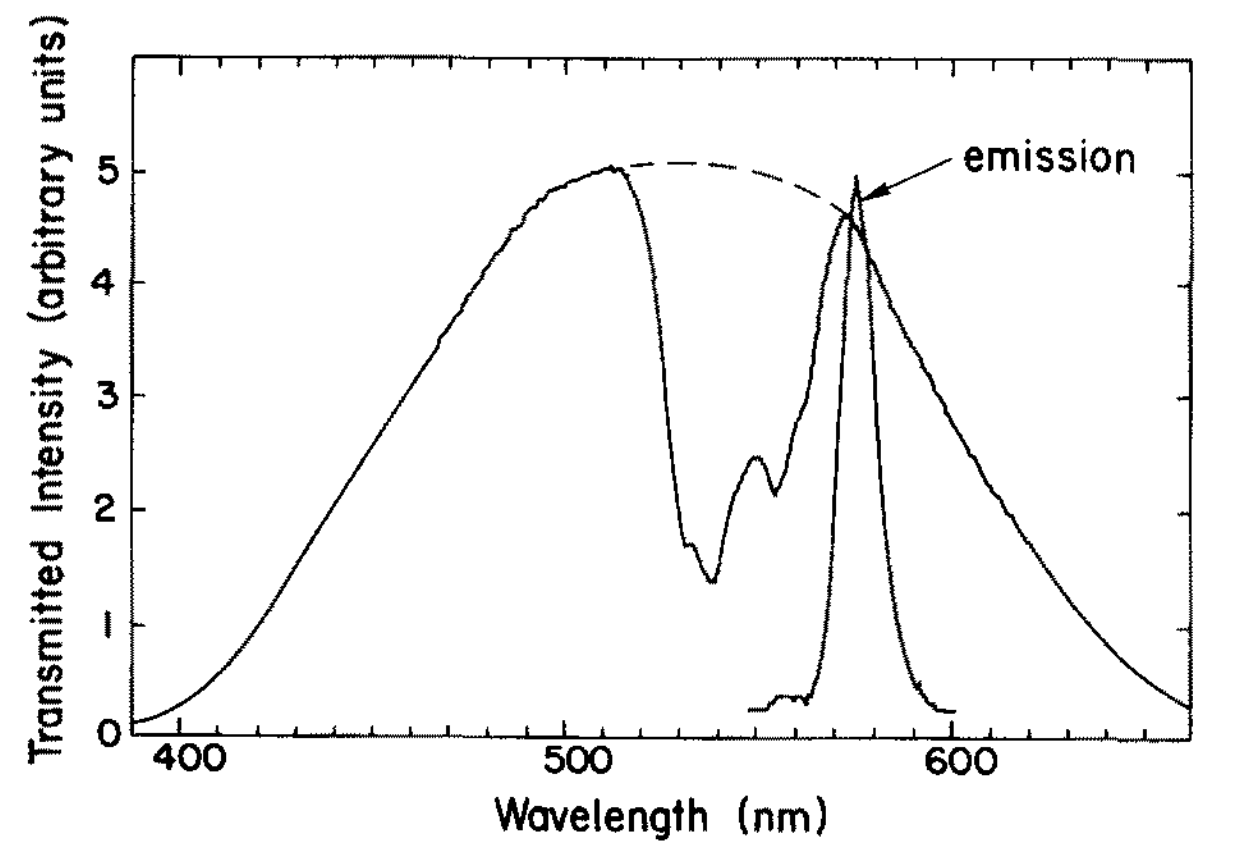
\includegraphics[width=.7\textwidth]{figures/Ba_in_SAr.png}
%                \caption{Absorption and emission spectra of neutral Ba in SAr at 10~K.  \cite{SAr}}
%\label{fig:BaSAr}
%\end{figure}

%Energy level transition probabilities can also be affected in a matrix.  If potential energy curves cross each other, non-radiative transitions can become allowed for otherwise forbidden transitions \cite{crepin}.  Spin-forbidden transitions, both radiative and non-radiative, between triplet and singlet states can become more significant for heavy host atoms like Xe \cite{heavyAtom}.  Effects like these could aid in observation of the Ba/Ba\textsuperscript{+}, e.g. by improving decay rates out of metastable D states, or they could reduce detectability, e.g. if a non-radiative decay competes with the fluorescence channel.

%, e.g., spin-forbidden transitions can become more significant via the heavy atom effect [ref...i know you have crepin but maybe you can use crepin's ref, since you need to understand this anyway]

%The detectability of a single atom/ion can depend greatly on [these]...

\section{Fluorescence Efficiency}
\label{sec:fluorEff}

The fluorescence efficiency ($\epsilon_{f}$) is the ratio of total fluorescence photons emitted to photons absorbed.  This can be calculated by Eq. \ref{eqn:flueEff}:

\begin{equation}
\epsilon_{f} = \frac{f}{W_{12} N_1 \epsilon_{\text{tot}}}
\label{eqn:flueEff}
\end{equation}
% = \frac{f h \nu}{\sigma I \epsilon_{c}}

\noindent
where $f$ is the number of fluorescence photons observed per atom per second, $W_{12} N_1$ is the excitation rate ($N_1 \approx 1$ for short times), and $\epsilon_{\text{tot}}$ is the photon detection efficiency of the system.  $W_{12}$ can be calculated by Eq. \ref{eqn:w12}.  The cross section can be calculated using the shape of an excitation spectrum according to Eq. \ref{eqn:sigma}:

\begin{equation}
\sigma(\nu) = A_{21} \frac{g_2}{g_1} \frac{c^2}{8 \pi \nu^2} g(\nu)
\label{eqn:sigma}
\end{equation}

\noindent
where $A_{21}$ is the atomic transition rate, $g_1$ and $g_2$ are the ground and excited state degeneracies, respectively, and $\nu$ is the photon frequency.  Here we have assumed that the integrated cross section is unchanged in the solid matrix as compared to in vacuum.  The normalized line shape $g(\nu)$ must satisfy:

\begin{equation}
\int_{0}^{\infty} g(\nu) d\nu = 1
\label{eqn:g}
\end{equation}

\noindent
Integrating Eq. \ref{eqn:sigma} then yields:

\begin{equation}
\int_{0}^{\infty} \sigma(\nu) \nu^2 d\nu = A_{21} \frac{g_2}{g_1} \frac{c^2}{8 \pi}
\label{eqn:sigma2}
\end{equation}

\noindent
Since the cross section $\sigma(\nu)$ is proportional to the excitation spectrum $E(\nu)$, we can finally write the cross section as a function of $\nu$ according to Eq. \ref{eqn:sigmafinal}:

\begin{equation}
\sigma(\nu) = \frac{A_{21} E(\nu)}{\int_{0}^{\infty} E(\nu') \nu'^2 d\nu'} \frac{g_2}{g_1} \frac{c^2}{8 \pi}
\label{eqn:sigmafinal}
\end{equation}
\chapter{Experimental}

%\emph{\color{gray}Probably need to mention CCD digitaztion pedestal and noise, and dark counts which are zero when cold -- did you do that?.}

%\noindent
%\emph{

In this chapter the apparatus at Colorado State University that was used for producing and observing  deposits of Ba and Ba\textsuperscript{+} in SXe is presented.  The main barium source, a Ba\textsuperscript{+} ion beam, is first described in Sec. \ref{sec:ionbeam}, and then a neutral Ba getter source is discussed in Sec. \ref{sec:getter}.  The co-deposit of Ba or Ba\textsuperscript{+} with Xe gas onto a cold sapphire window is described in Sec. \ref{sec:deposition}.  The technique for focusing the laser into the SXe is outlined in Sec. \ref{sec:laser}, and imaging of the laser region is described in Sec. \ref{sec:collection}, with attention to the effect of vibrations in Sec. \ref{sec:vibes}.  Finally, a system for scanning the focused laser across the sapphire window is discussed in Sec. \ref{sec:laserscanning}.

\section{Ion Beam System}
\label{sec:ionbeam}

The Colutron ion beam system is a clean mass-selected source of Ba\textsuperscript{+} which, with the added capability of pulsing, can do a very wide range of deposit sizes, from billions of ions in a focused laser region all the way down to the single-ion level and below.  The different components of this system are shown in Fig. \ref{fig:ionbeam} and described in the following subsections.  Ions produced in a Colutron ion source are accelerated and collimated for passage through the mass filter.  Several sets of deflection plates are available for steering, and Einzel lenses focus the beam near the final Faraday cup.  A set of pulsing plates can be used to deposit 1-$\mu$s ion pulses in SXe on the cold sapphire window, or continuous ion current can be used in depositing larger numbers of ions.
%(may only want to say that if we have those scans)

\vspace{20mm}

%\begin{landscape}
\begin{figure} %[H]
        \centering
                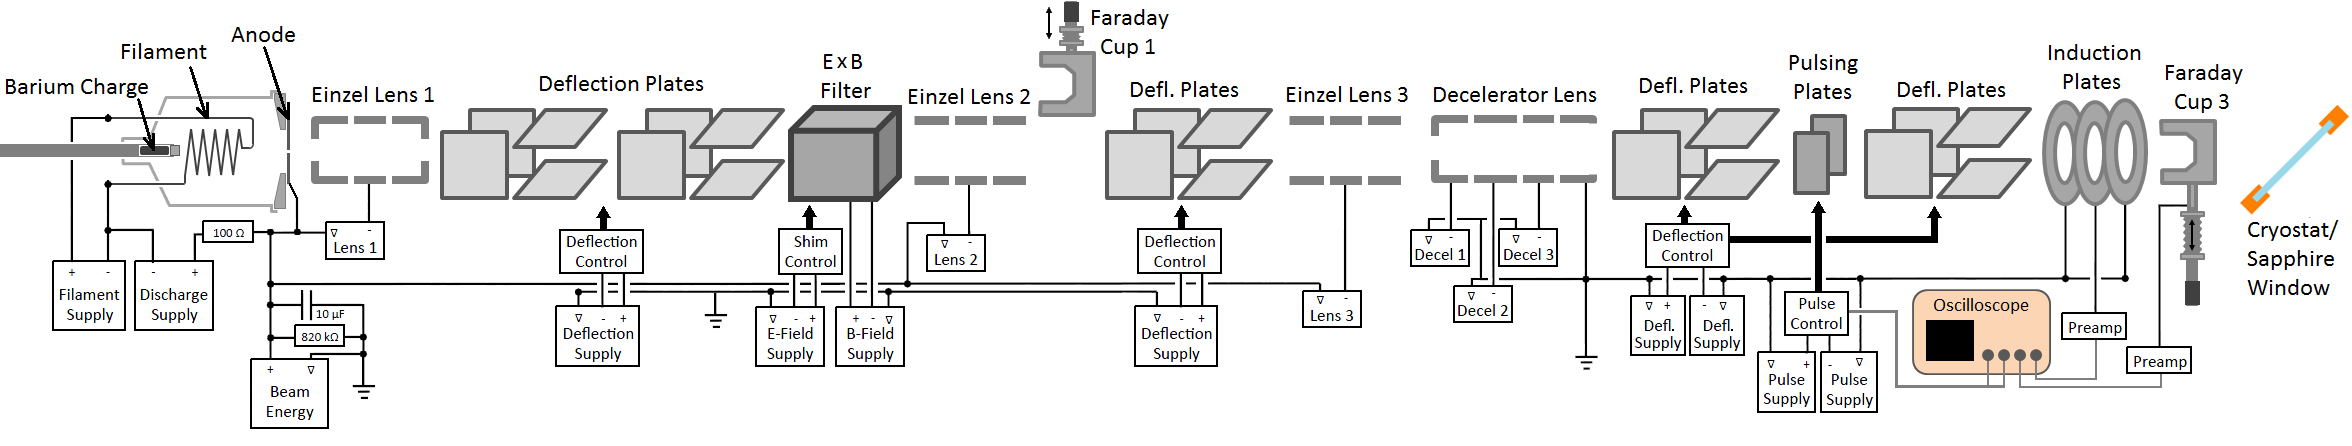
\includegraphics[angle=90,width=.25\textwidth]{figures/ionBeam.png} %angle=90,
                \caption{Ba\textsuperscript{+} ion beam system.}
\label{fig:ionbeam}
\end{figure}
%\end{landscape}
%width=1.4 is good for landscape, but idk how to get it in the center

\subsection{Ion Source}

Ba\textsuperscript{+} ions are produced in the source of a Model DCIS-101 Colutron ion gun \cite{Colutron}.  It is shown in Fig. \ref{fig:ionsource}.  A solid Ba charge is placed into the hollowed end of a stainless steel rod, which is capped by a loose screw.  The source rod is inserted into the discharge chamber, where it is heated by a filament, vaporizing the Ba.  The source is designed to produce a discharge between the anode plate and the filament cathode, through an argon buffer gas leaked into the source chamber.  This controlled discharge also ionizes Ba atoms in the vapor to produce the desired Ba\textsuperscript{+} ion beam.  In the present work, to avoid contamination of the SXe matrix with residual Ar gas, the buffer gas was not used.  It has been found that, with care, the discharge can be maintained with Ba vapor alone.  The longevity of ion current from a single charge is at least several 10s of hours.  This suggests that Ba is coating the inner walls of the source chamber, and is heated enough to provide sufficient Ba pressure to support a discharge.

The discharge produces a plasma, containing barium ions.  The application of a 2~kV acceleration potential between the ion source anode and the first element of Einzel lens 1 (L1) draws Ba\textsuperscript{+} ions from the plasma.  The potential of this lens is adjusted to collimate the ion beam for passage through the E$\times$B velocity filter.

%This is supported by the observation of white oxidation of the inner source parts after a few minutes of exposure to air when opening the system.

\begin{figure} %[H]
        \centering
                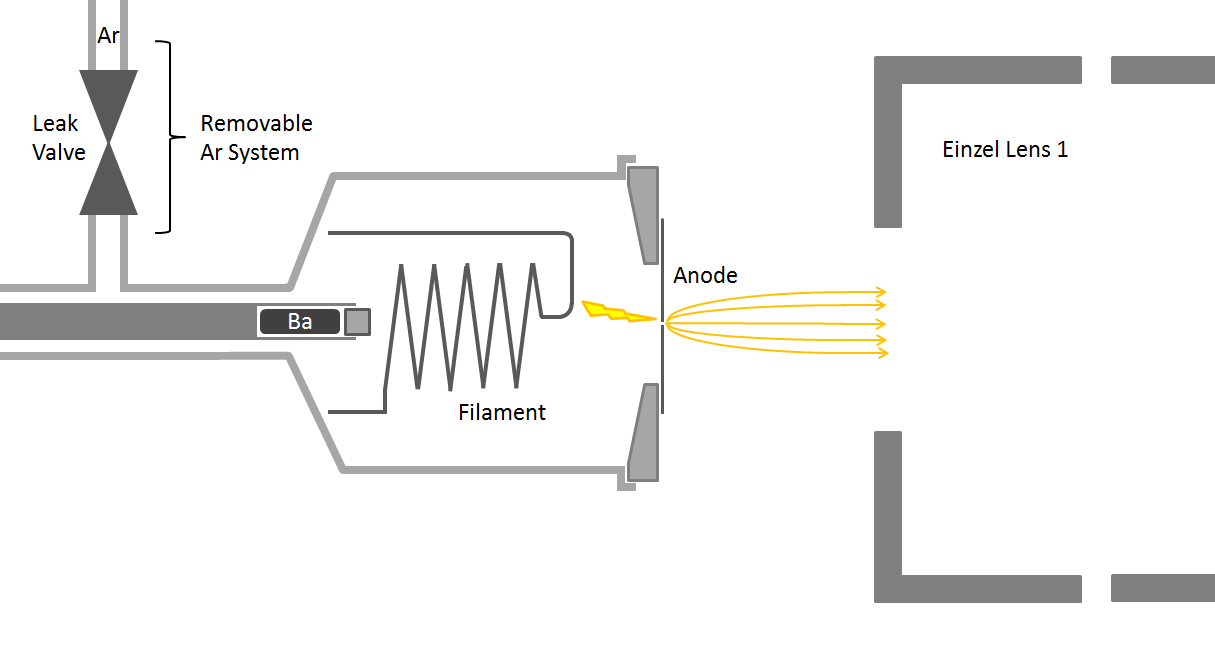
\includegraphics[width=.95\textwidth]{figures/ionSource.png}
                \caption{Ba\textsuperscript{+}/Ar\textsuperscript{+} ion source.}
\label{fig:ionsource}
\end{figure}

\subsection{E$\times$B Velocity Filter}

The E$\times$B velocity filter selects Ba\textsuperscript{+} by creating perpendicular electric and magnetic fields, which produce opposing forces on charged particles moving through the filter.  The opposing forces will be equal for ions with velocity $v = \frac{E}{B}$.  Since ion velocity is determined by mass ($m$), charge ($q$) and beam potential ($V$), the filter selects ions satisfying Eq. \ref{eqn:massfilt}:

\begin{equation}
\frac{m}{q} = \frac{2 V B^{2}}{E^{2}}
\label{eqn:massfilt}
\end{equation}

\noindent
where $B$ and $E$ are the magnetic and electric fields, respectively.  Those fields are chosen such that Ba\textsuperscript{+} ions pass straight through.  Other ions, e.g. Ar\textsuperscript{+}, will be deflected.  

The E$\times$B filter is shown in Fig. \ref{fig:exb}.  Electromagnets provide a vertical magnetic field.  Electrode plates and field-shaping guard rings provide a horizontal electric field.  The guard rings prevent lensing and astigmatism from fringe fields of the plates \cite{Colutron}.

\begin{figure}[h]
        \centering
                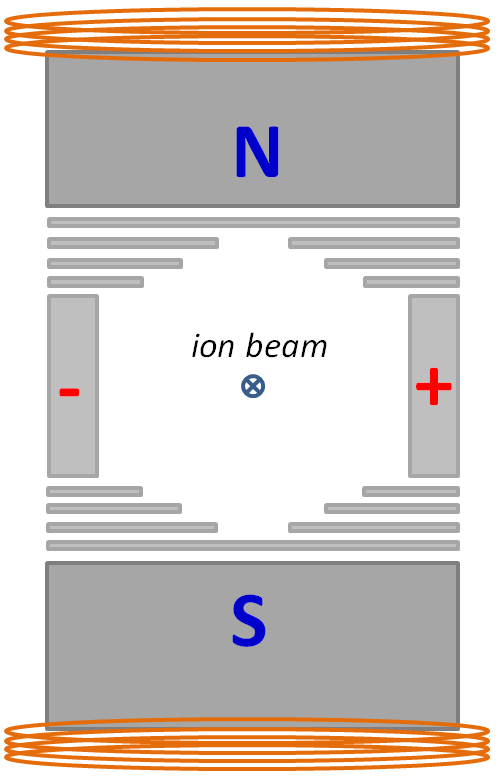
\includegraphics[width=.7\textwidth]{figures/ExB.png}
                \caption{Colutron E$\times$B ion velocity filter.}
\label{fig:exb}
\end{figure}

%\emph{\color{gray}If we need mass scans, we probably need to do new ones with a constant magnetic field, and Ar\textsuperscript{+} and Ba\textsuperscript{+} in same day.  Past scans were all over the place, partly because we were changing beam settings, but new peaks are not very consistent either.}
%To determine the mass components of the beam, the electric field can be scanned.  Mass scans of the Ba\textsuperscript{+} beam is shown in Fig. [ref mass scan fig], as well as of an Ar\textsuperscript{+} beam.  The known mass of Ar aids in calibrating the magnetic field, which differs from the calculation given by Colutron, likely due to hysteresis in the magnet.  \emph{\color{gray}The Ba\textsuperscript{+} peak agrees with the Ba mas s... }

\subsection{Other Beam Components}

The first three sets of deflection plates shown in Fig. \ref{fig:ionbeam} can be used for beam diagnostics, and are set to 0~V during normal operation.  The fourth set of deflection plates, H1 and V1, located just before the pulsing plates, are set to constant values of +50~V and 0~V, respectively.  These voltages have been selected such that the beam, in both pulsing and continuous modes, can be deposited at the sapphire window for reasonable settings on the final deflection plates, H2 and V2.  As described in Section \ref{subsec:ionDepCal}, different settings in H2/V2 are required for peak ion current in Faraday cup 3 vs. peak deposit at the window.

Einzel lens 2 (L2) focuses the beam to pass through the aperture in the first element of the decelerator lens.  Einzel lens 3 (L3) is set to zero in this setup.  If desired, the decelerator lens can be used to vary the Ba\textsuperscript{+} deposit energy, which was done in \cite{Shon}, but in this work it acts as an Einzel lens with only the second element (D2) at non-zero voltage.  It focuses the beam near the sample and Faraday cup 3 (there is no Faraday cup 2 in this setup).

Faraday cup 3 measures the ion current during experiments, and is retracted when deposits are being made.  Calibration of deposits using Faraday cup 3 is described in Section \ref{subsec:ionDepCal}.  Faraday cup 1 can be used for beam diagnostics, and is usually retracted.  An additional Faraday cup, cup W, can be attached to the coldfinger in place of the sapphire window for determining optimum deflection plate voltages for depositing Ba\textsuperscript{+} on the sapphire window, and for calibrating ion deposits.  This is described further in Sec. \ref{subsec:ionDepCal}.

To align the ion beam, L1 was first tuned to maximize ion current in Faraday cup 3, with L2, L3, and D2 set to zero.  Since cup 3 is about 2~m away from L1, this approximately collimates the beam for passage through the E$\times$B filter.  The optimal value for L1 was found to be around -400~V relative to the 2000~V beam energy.  Next, L2 and D2 were fine-tuned together to achieve maximal current in cup 3.  Finally, the straightness of the beam was checked by peaking ion current with the final four deflection plates on cup 3 and cup W.

%\emph{\color{red}consistent with Bill's SIMION -- show?}

%L2 8.34 = 

\subsection{Ion Beam Pulsing}

To deposit small numbers of ions, it is desirable to be able to pulse the ion beam with short pulses.  To achieve pulsed beams, the pulsing plates, normally set to 200~V and -200~V to deflect the beam, are pulsed to 0~V for 1~$\mu$s to pass a short pulse of ions straight forward.  The pulsing circuit is shown in Fig. \ref{fig:pulse_circuit}.  Square waves, triggered by LabVIEW at 500~Hz, enter the circuit at (a). A transformer isolates a MOSFET switch from ground.  Upon a trigger pulse the MOSFET switch shorts the pulsing plates for the period of the pulse.

\begin{figure} %[h]
        \centering
                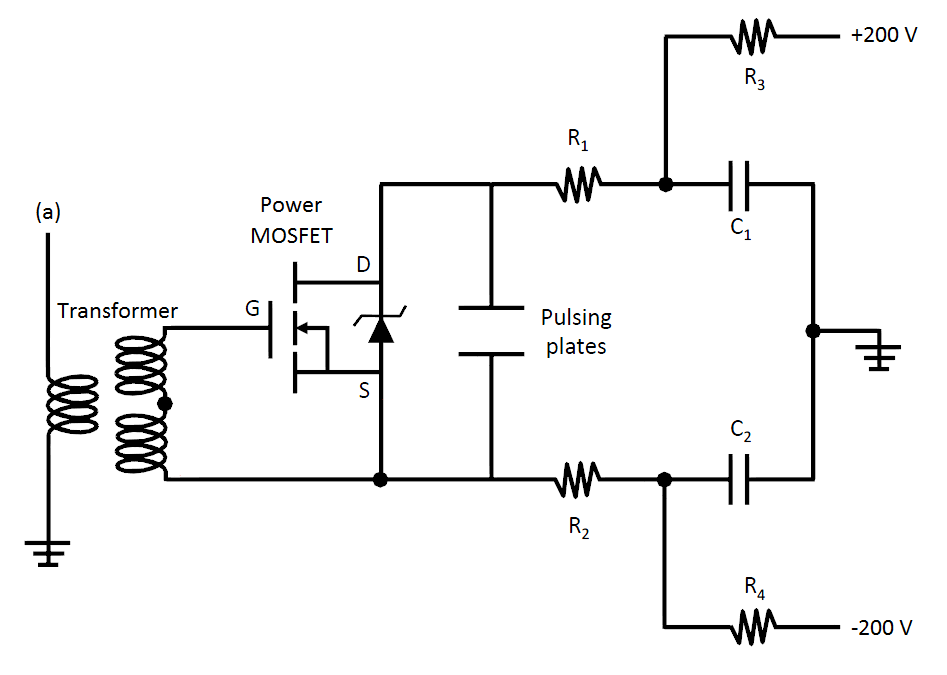
\includegraphics[width=.85\textwidth]{figures/pulsing_circuit.png}
                \caption{Pulsing circuit.  R$_{1}$ = R$_{2}$ = $470~\Omega$, R$_{3}$ = R$_{4}$ = 20~k$\Omega$, and \newline C$_{1}$ = C$_{2}$ = 680~nF. \cite{Shon}}
\label{fig:pulse_circuit}
\end{figure}

The pulsing plates are followed by three induction plates, the middle plate of which provides a measure of the ion pulses.  Just prior to a deposit, the charge in the pulses can be directly measured on cup 3.  eV Products pre-amplifiers convert the ion current in the induction plates and cup 3 (or cup W) to voltage signals, which are recorded on a digital oscilloscope.  An example of raw oscilloscope traces of Faraday cup 3 and induction plate signals are shown in Fig. \ref{fig:pulse_raw_shaped}(a).  The input current is related to the pre-amp output voltage according to Eq. \ref{eqn:preamp}:

\begin{equation}
I = \frac{-(V_{out} + R_{1} C \frac{dV_{out}}{dt})}{R_{1} M}
\label{eqn:preamp}
\end{equation}

\noindent
where $R_{1} C$ and $R_{1} M$ are determined by putting a known square pulse of current into the pre-amp through a large resistor.  First, the time constant of an exponential fit to the signal decay after the pulse determines $R_{1} C$.  Then $R_{1} M$ is determined by matching the amplitude of the calculated current signal to the original square-pulse input current.  The actual currents in the induction plates and cup 3 calculated using Eq. \ref{eqn:preamp} are shown in Fig. \ref{fig:pulse_raw_shaped}(b).  The induction signal is positive as ions are approaching the middle plate, and an equal but negative signal is seen after the ions pass this plate.  The Faraday cup stops the ions, so it produces only a positive induction signal as ions approach it.

\begin{figure} %[H]
        %\centering
        %\begin{subfigure}
                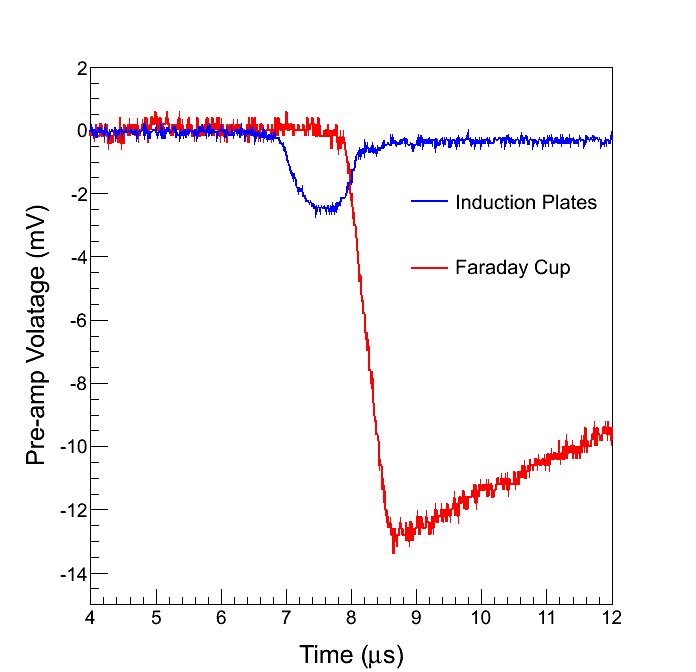
\includegraphics[width=.49\textwidth]{figures/pulse_ind_cup3_raw.png}
                %\caption{barf}
%        %\end{subfigure}
        %\begin{subfigure}
                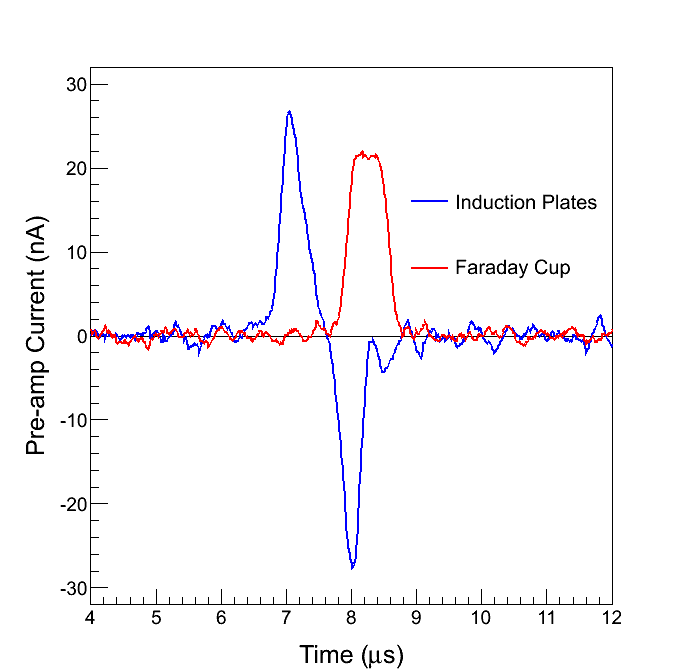
\includegraphics[width=.49\textwidth]{figures/pulse_ind_cup3_shaped.png}
                \caption{Raw voltage (a) and calculated current (b) pulse signals from the induction plates and cup 3.  The raw induction signal appears small because it has a less sensitive pre-amp (accounted for in calculating the current).}
        %\end{subfigure}
        \label{fig:pulse_raw_shaped}
\end{figure}

Pulsing data also provide confirmation that the beam is composed of Ba\textsuperscript{+}.  The time between the pulsing plate voltage peaks and the center of the pulse measured by the Faraday cup, along with the known distance traveled, determines the velocity of the ions.  The distance from the center of the pulsing plates to the Faraday cup was measured to be 31.5 $\pm$ 0.5~cm.  Time-of-flight data, e.g. Fig. \ref{fig:pulses_ArBa}, give 39.8 $\pm$ 3.4~amu for Ar\textsuperscript{+} ions and 136.8 $\pm$ 6.3~amu for Ba\textsuperscript{+} ions, including an uncertainty on the time of flight of $\pm$ 0.1~$\mu s$.  These agree with the known atomic masses.

\begin{figure}[h]
        \centering
                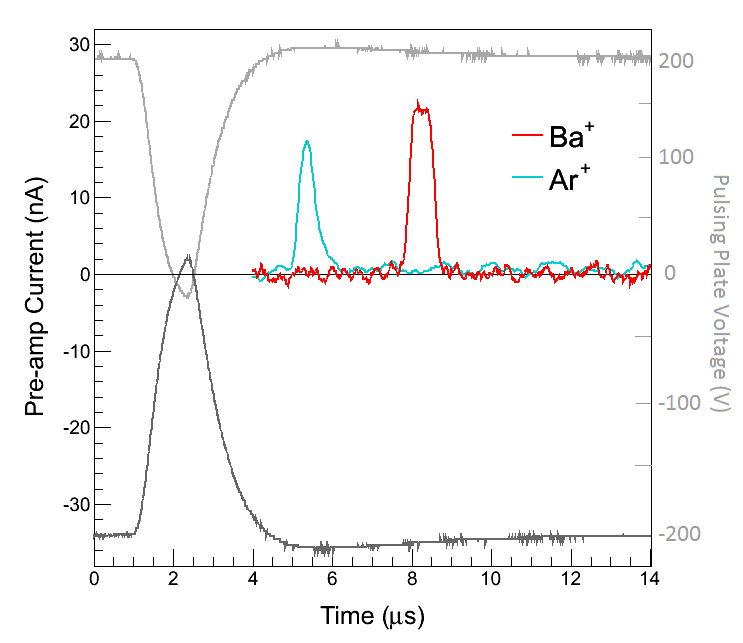
\includegraphics[width=.7\textwidth]{figures/pulses_BaAr.png}
                \caption{Arrival time of pulses at cup 3 vs. time of pulsing plate signal (black (+) and gray (-)) for Ar\textsuperscript{+} and Ba\textsuperscript{+} ions at 2000~eV.}
\label{fig:pulses_ArBa}
\end{figure}

\subsection{Calibration of Ion Deposits}
\label{subsec:ionDepCal}

The ratio of between the continuous ion currents in cup 3 and cup W was typically measured to be $r_{\text{w}} = 0.5$.  As the ion beam at cup W is significantly wider than the cup diameter and is thought to be fairly uniform, the ion density per pulse at the sapphire window is given by:

\begin{equation}
\frac{\text{ions}}{\text{pulse} \times m^{2}} = \frac{Q r_{\text{w}}}{e A}
\label{eqn:ion_density}
\end{equation}

\noindent
where $Q$ is the charge/pulse at cup 3, $A$ is the area of cup W, and $e$ is the elementary charge.  The radius of the opening in cup W is 1.4~mm.  Each time cup W is inserted, the voltages on the final deflection plates H2 and V2 that optimize the signal in cup W, in pulsed and in continuous mode, are determined.  In the latest imaging experiments, these differed from the values for maximum cup 3 signal by about 70~V in H2 and 60~V in V2, corresponding to a displacement of the undeflected beam of about 4~mm in x and y position at cup W relative to the center line from cup 3.  This indicates the level of drift in optimal ion beam component settings that occur over a long period of time.

\section{Ba Getter Source}
\label{sec:getter}

A BaAl$_{4}$ getter (SAES with part number ST 2/F/WIRE), can be inserted on a bellows to emit Ba atoms toward the sapphire window, as shown in Fig. \ref{fig:endOfBeamBa}.  When heated, the getter emits neutral Ba with minimal Ba\textsuperscript{+} content due to the low temperature ($\sim$800$^{\circ}$ C determined by observing brick red color temperature).  Getters were used extensively in previous work \cite{Brian} for measuring the absorption and emission spectra of Ba in SXe with large Ba deposits.  A getter was used briefly in this work in verifying that the 619-nm fluorescence peak, that is used for single Ba imaging, is actually a neutral Ba peak, as described in Section \ref{sec:619identification}.  The barium getters used in \cite{Brian} were exothermic BaAl$_{4}$-Ni flash getters.  The getter used here is an endothermic BaAl$_{4}$ type, designed for more controlled Ba emission.  

%no evidence is provided in Brian's thesis, nor Shon's, and I don't see anything on the SAES website

\begin{figure} %[h]
        \centering
                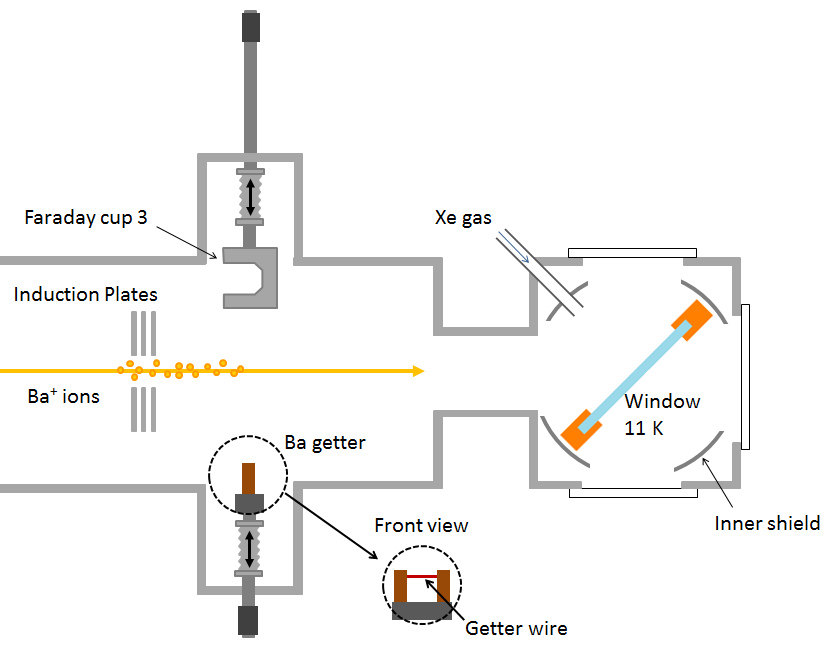
\includegraphics[width=.75\textwidth]{figures/window_etc_justBa_frontViewGetter.png}
                \caption{Apparatus near sapphire window, including induction plates, Ba getter, Faraday cup 3, Xe gas inlet, and sapphire window at 11~K.}
\label{fig:endOfBeamBa}
\end{figure}

%\begin{figure} %[h]
%        \centering
%                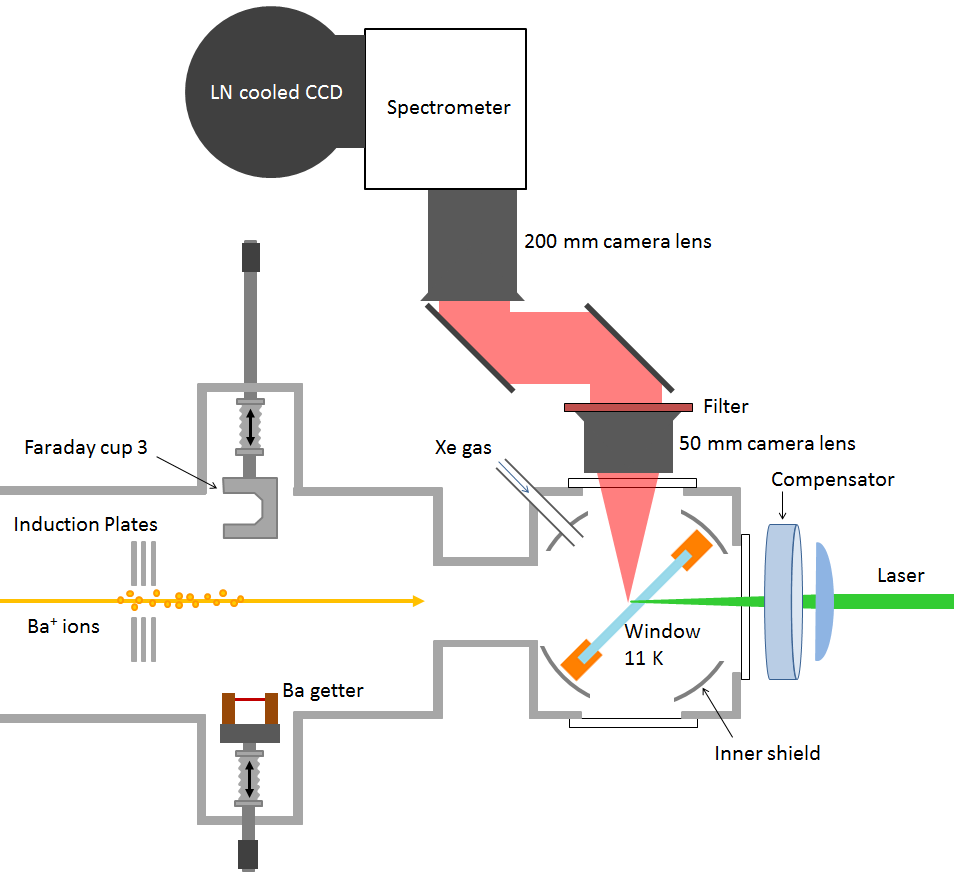
\includegraphics[width=.9\textwidth]{figures/window_etc.png}
%                \caption{Apparatus in spectroscopy region, including Ba getter, Faraday cup 3, induction plates, and optics for excitation, fluorescence collection, spectroscopy and detection.}
%\label{fig:endOfBeam}
%\end{figure}

\section{Sample Deposition}
\label{sec:deposition}

The Ba\textsuperscript{+}/Ba is co-deposited with 99.995\% purity Xe gas onto a cold sapphire window.  Sapphire has good thermal conductivity at low temperature and good optical transparency in the visible.  The window is held in a copper mount attached to a coldfinger and is tilted at 45$^{\circ}$ to allow access of the ion beam and Xe gas, as well as the excitation laser and collection optics.  To begin a deposit, Xe gas is flowed toward the window via a leak valve, through an inlet system designed and built by Brian Mong and Shon Cook \cite{Brian,Shon}.  Cup 3 is then retracted and the pulsing plates are pulsed to zero volts, depositing 1-$\mu$s pulses of Ba\textsuperscript{+} ions into the SXe matrix as it grows.  Cup 3 is then replaced, and the Xe leak stopped.

\begin{figure} %[h]
        \centering
                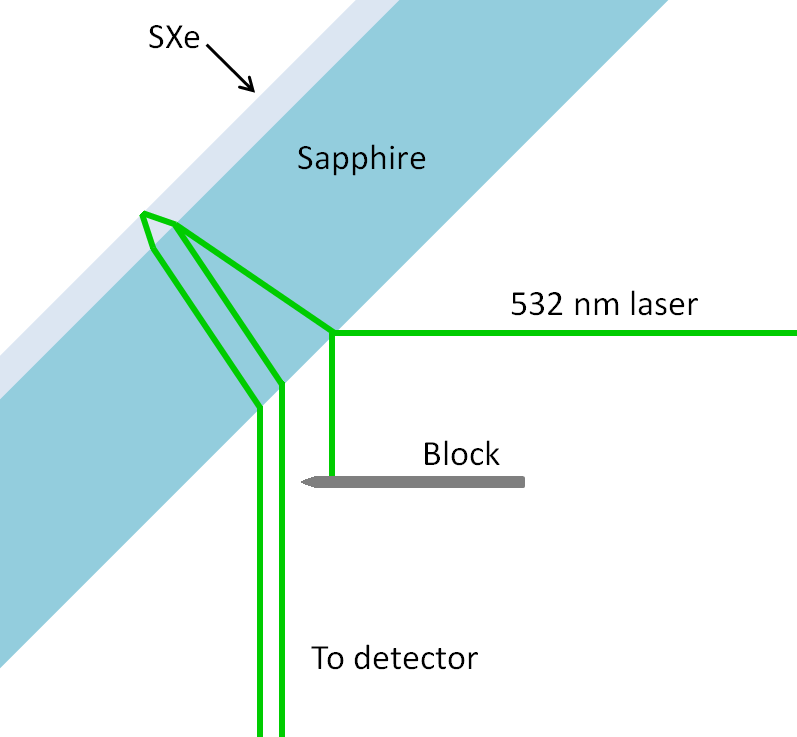
\includegraphics[width=.4\textwidth]{figures/fringe_setup.png}
                \caption{Setup for measuring SXe deposition rate by interference fringes.}
\label{fig:fringe_setup}
\end{figure}

\begin{figure} %[h]
        \centering
                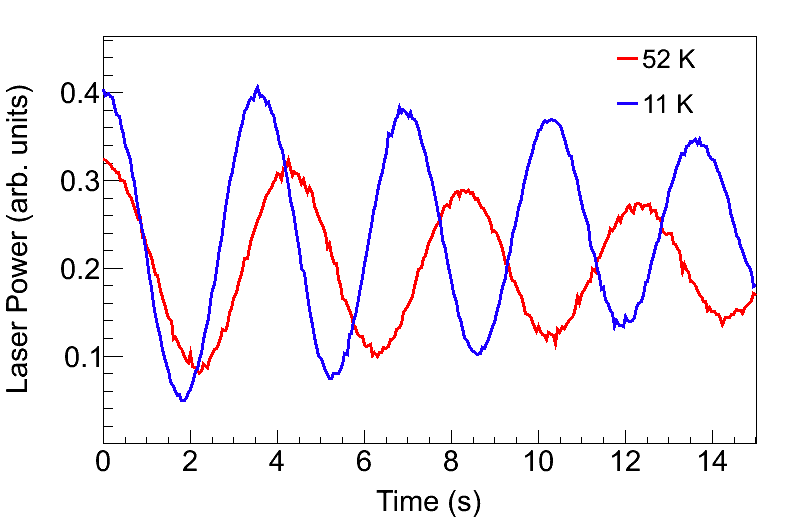
\includegraphics[width=.5\textwidth]{figures/fringes_52K_vs_11K.png}
                ~
                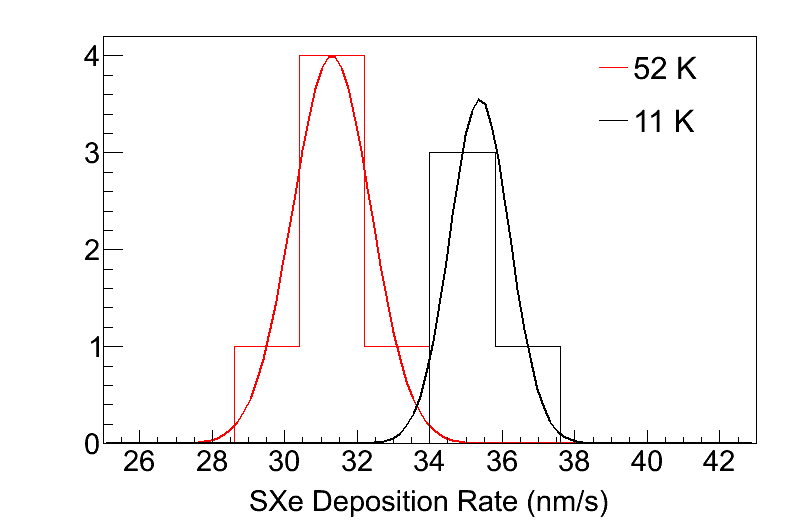
\includegraphics[width=.5\textwidth]{figures/fringes_52K_vs_11K_statistics.png}
                \caption{(a) Interference fringes for the same Xe gas leak rate deposited on the sapphire window at 11~K and at 52~K, and (b) distribution of SXe deposition rates calculated from fringe period of several measurements.}
\label{fig:fringes_52K_vs_11K}
\end{figure}

The SXe matrix deposition rates have been measured by interference fringes in a 532-nm laser reflected from the front surface of the sapphire window and the SXe surface, as shown in Fig. \ref{fig:fringe_setup}.  Fringes for SXe deposition at 52~K and 11~K are shown in Fig. \ref{fig:fringes_52K_vs_11K}(a) for the typical leak rate used in this work.  The refractive index of SXe has a negligible dependence on temperature between 50~ and 30~K \cite{SXeIndex}, so these rates can be compared directly.  A distribution of SXe deposition rate measurements from several deposits is shown in Fig. \ref{fig:fringes_52K_vs_11K}(b).  A rate of $31.2 \pm 0.9$~nm/s is measured for deposits at 52~K, and a somewhat higher rate of $35.6 \pm 0.9$~nm/s is measured for deposits at 11~K.

%A somewhat lower rate is observed at 52~K, $31.3 \pm 0.44(\text{stat}) \pm 0.31(\text{sys})$~nm/s, vs. $35.4 \pm 0.41(\text{stat}) \pm 0.35(\text{sys})$~nm/s at 11~K.  Statistical errors are $\sigma / \sqrt{N}$ where $\sigma$ is the standard deviation of the Gaussian fits to the distributions in Fig. \ref{fig:fringes_52K_vs_11K}(b), and $N$ is the number of entries.  Systematic errors come from propagating an uncertainty on the angle between the laser and sapphire window of $\pm 2^{\circ}$.

\begin{figure} %[h]
        \centering
                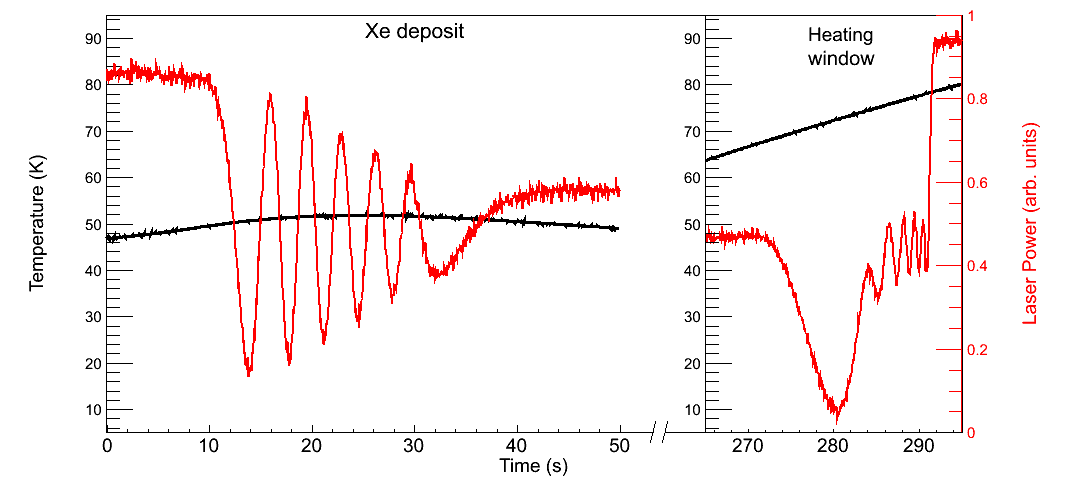
\includegraphics[width=.9\textwidth]{figures/fringes_dep_and_melt.png}
                \caption{Interference fringes (red) of a SXe deposit at 52~K and of its subsequent evaporation when heating the sapphire window, and temperature (black) vs. time.}
\label{fig:fringes_melt_withDep}
\end{figure}

To evaporate a sample, the window is heated to 100~K.  Fringes appear during this process as well.  The full set of fringes for a deposit at 52~K and during its evaporation when heated is shown in Fig. \ref{fig:fringes_melt_withDep}, along with the window temperature.  It is observed that the SXe evaporates between 73~K and 78~K.  The same number of fringes appear in the deposit and the evaporation, indicating that the lower deposition rate at around 50~K is not due to simultaneous evaporation, but perhaps it is due to a different sticking coefficient.  The variation in temperature during the deposit is due to the heater cycle.  These Xe deposits were for a longer time than in a typical deposit during a fluorescence experiment, in order to observe several fringes.

%quadrature errors: 0.54 for 52 K and 

%where sh'ew put this? sh'we?  these numbers are apparently wrong anyway   {\color{red}Using the 10~K SXe density of 3.780~g/cm\textsuperscript{3} \cite{SXeDensity} and a typical Ba\textsuperscript{+} ion current density of 1.6~nA/mm\textsuperscript{2} at the sapphire window, \emph{\color{gray}Re-do this, ala procedure in thought\_process.pptx, since you don't claim 37 nm/s anymore:} 5~nm/s \emph{\color{gray}any other instances?} and 37~nm/s correspond to Xe:Ba ratios of about $8.7 \times 10^{3}$ and $6.4 \times 10^{4}$ respectively.  Xe leak rates above 37~nm/s result in rapid frosting of the SXe matrix, which causes blurring of the image and high laser scatter.}

\section{Laser Excitation}
\label{sec:laser}

\begin{figure} %[h]
        \centering
                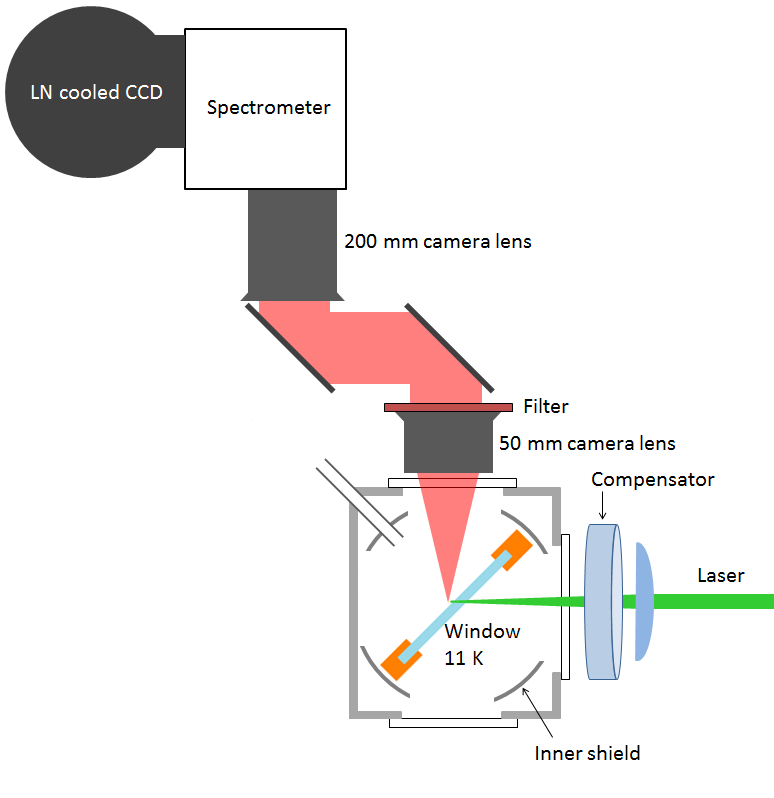
\includegraphics[width=.7\textwidth]{figures/window_etc_justOptics.png}
                \caption{Apparatus in spectroscopy region, including optics for excitation, fluorescence collection, spectroscopy and detection.}
\label{fig:endOfBeamOptics}
\end{figure}

Green to yellow laser excitation is done with a Coherent 599 dye laser, pumped by the 514-nm line of a Lexel 3500 Ar ion laser.  Rhodamine 110 (R110) dye is used for the 542 - 566~nm wavelength range, and Rhodamine 6G (R6G) for the 567 - 590~nm range.  Another Coherent 599 dye laser with Coumarin 480 (C480) dye, pumped by a Kr ion laser., is used for blue excitation.  The Coherent 599 dye lasers are used with birefringent filters for wavelength tuning, but without etalons or single frequency stabilization, since the broad absorption of Ba and Ba\textsuperscript{+} in SXe does not require narrow band laser excitation.

\begin{figure} %[h]
        \centering
                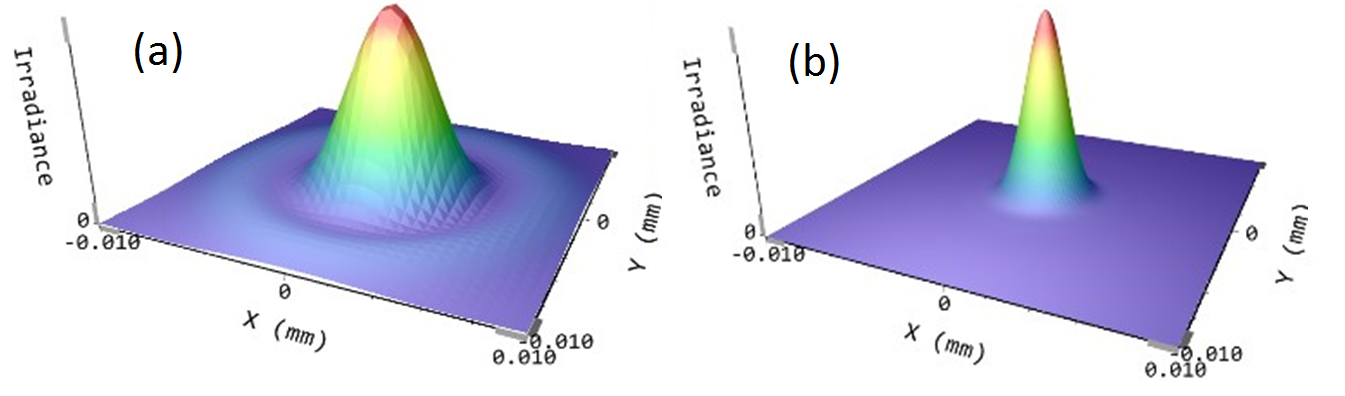
\includegraphics[width=.7\textwidth]{figures/DFairbank_aber.png}
                \caption{Calculated minimum laser spot size distributions, with wavelength 570~nm and incident laser radius w = 7~mm, for (a) bi-convex f = 7~cm lens, and (b) aspherical f = 7.9~cm lens.  \cite{DFairbank}}
\label{fig:DFairbank}
\end{figure}

The optics for these experiments is shown in Fig. \ref{fig:endOfBeamOptics}.  In initial work, including spectroscopy (Chapter \ref{chapter:spectroscopy}) and some imaging (Chapter \ref{chapter:imaging}), a bi-convex was used.  This lens had a little spherical aberration, resulting in blurring of the laser focus.  This aberration does not affect the spectroscopy results in Chapter \ref{chapter:spectroscopy}, where semi-focused beam 1/$e^{2}$ radii of 100-1000~$\mu$m were used.  However, spherical aberrations caused the minimum beam radius to be about 5~$\mu$m.  To approach the diffraction limit in imaging small numbers (Chapter \ref{chapter:imaging}), a 7.9-cm focal length aspherical lens was used.  A comparison of the minimum spot sizes for these two lenses, calculated by David Fairbank of Thorlabs with OpticStudio software, is shown in Fig. \ref{fig:DFairbank}.

\begin{figure} %[H]
        \centering
                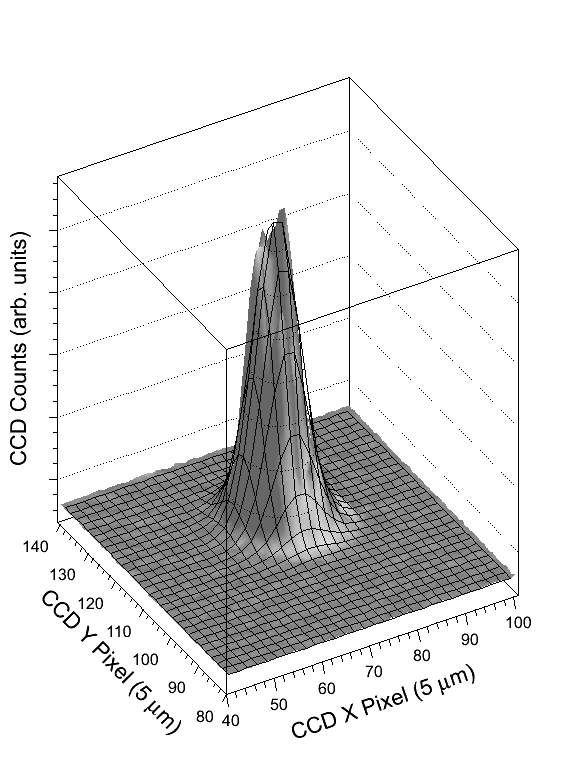
\includegraphics[width=.33\textwidth]{figures/astig_thesis_2Dgaus_run35.png}
                ~
                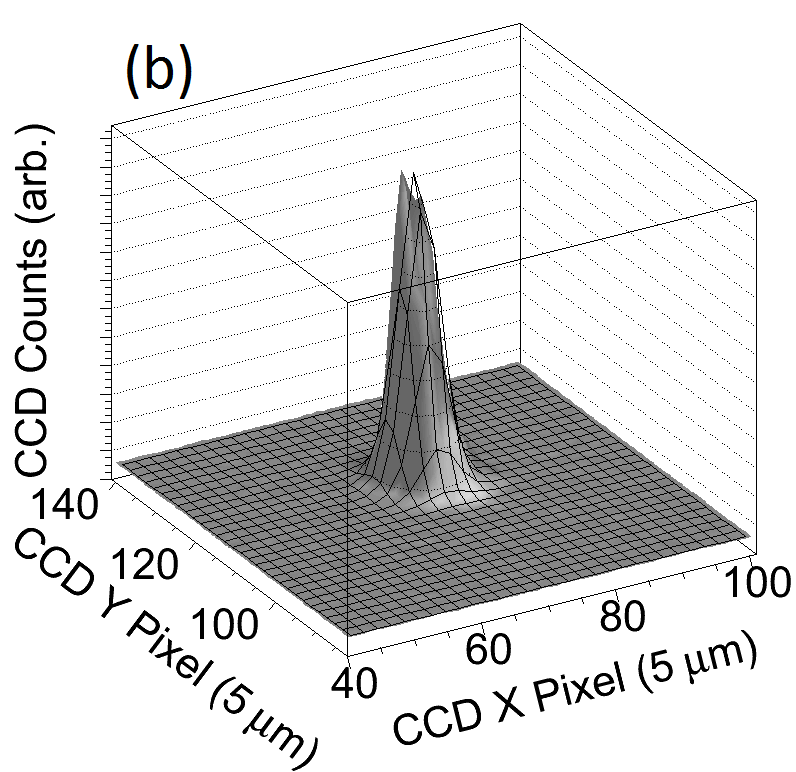
\includegraphics[width=.33\textwidth]{figures/astig_thesis_2Dgaus_run39.png}
                ~
                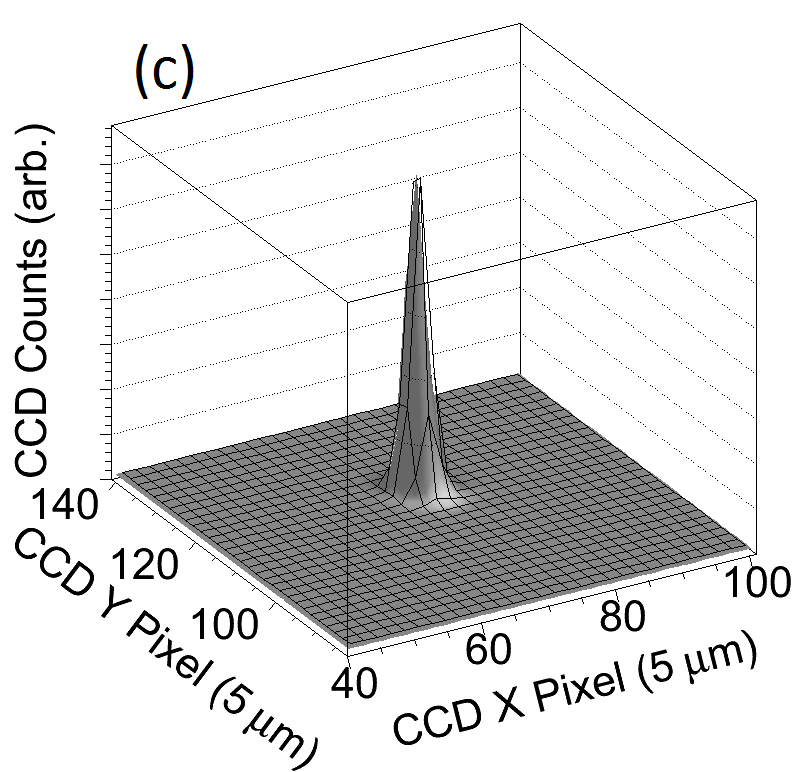
\includegraphics[width=.33\textwidth]{figures/astig_thesis_2Dgaus_run43.png}
                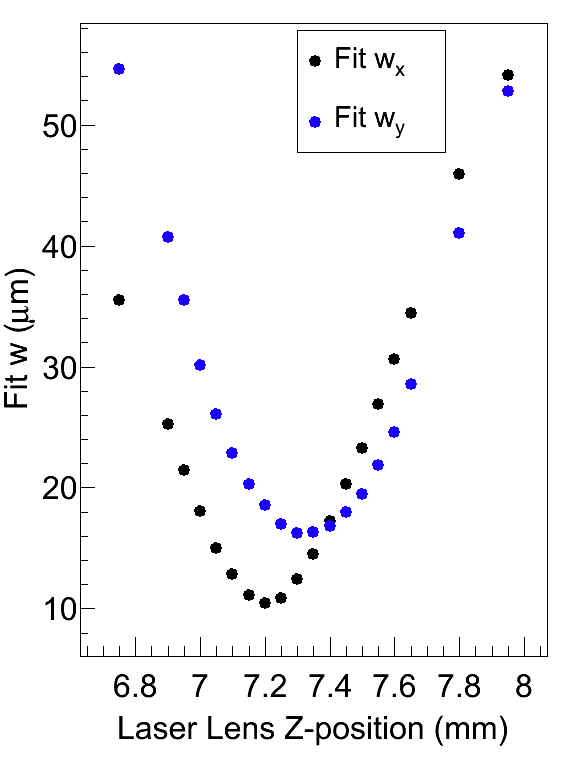
\includegraphics[width=.45\textwidth]{figures/astigcorr_curve_no-corr_806.png}
                ~
                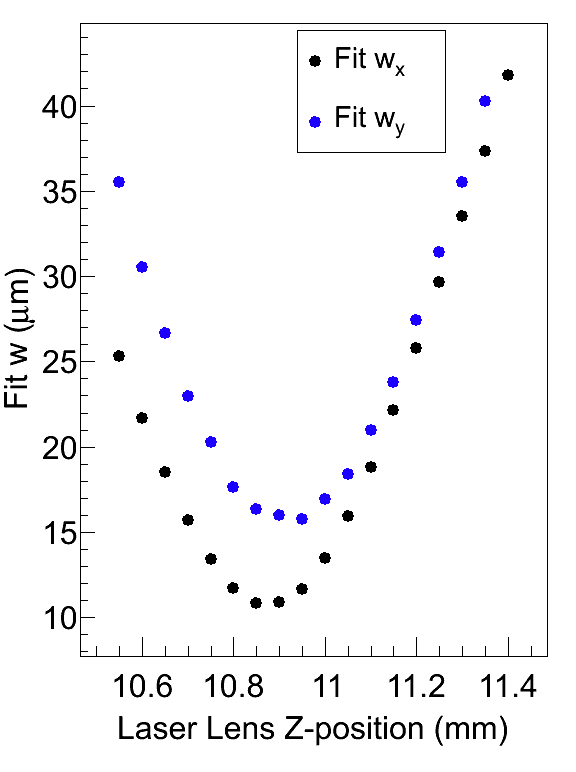
\includegraphics[width=.45\textwidth]{figures/astigcorr_curve_corr_10deg.png}
                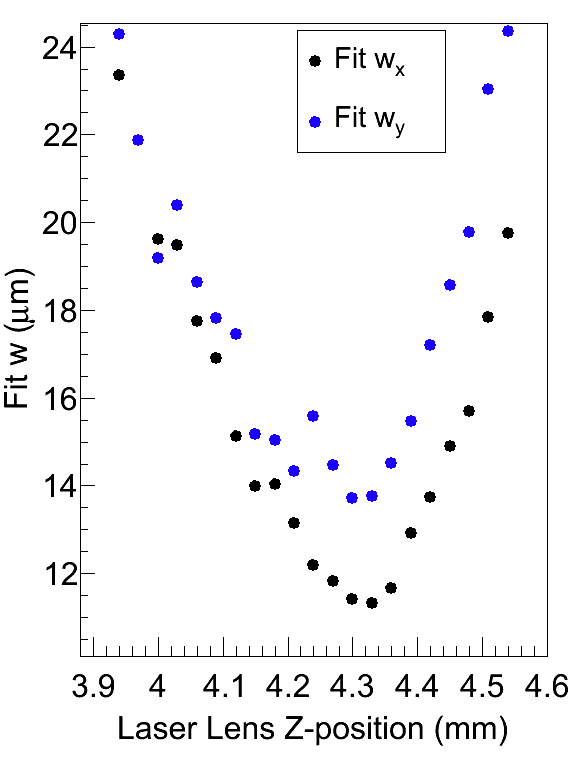
\includegraphics[width=.45\textwidth]{figures/astigcorr_curve_corr_9-16.png}
                ~
                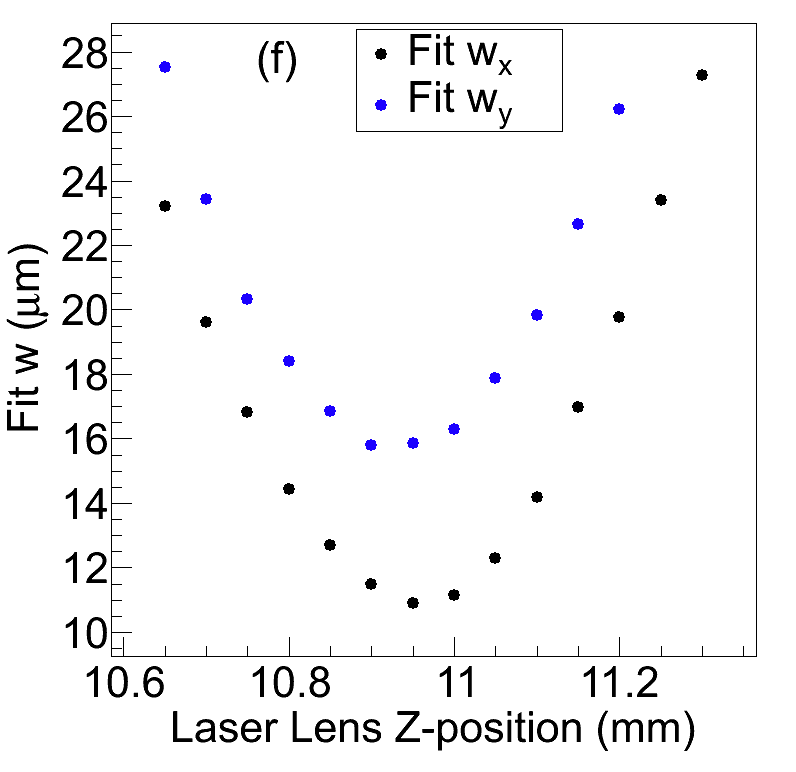
\includegraphics[width=.45\textwidth]{figures/astigcorr_curve_corr_13deg.png}
                \caption{Example 2D Gaussian fits (black grid lines) with varying laser z position (a,b,c), and fit radii  w$_{\text{x}}$ (black) and  w$_{\text{y}}$ (blue) vs. laser focus lens position with (d) no compensator, and with compensator at about (e) 10$^{\circ}$, (f) 11$^{\circ}$, and (g) 13$^{\circ}$.}
\label{fig:astig}
\end{figure}	

The tilted sapphire window introduces astigmatism to the focused laser.  To correct for this, compensating astigmatism is introduced by a fused silica optical flat of 1~cm thickness, placed after the lens, with surfaces normal to the horizontal xz plane, tilted in the xz plane (the laser is along the z-direction, and the sapphire window is tilted in the vertical yz plane).  The proper angle for the compensator was determined to be about 10$^{\circ}$ from normal by a ray matrix calculation \cite{raymatrix}.  The effect of astigmatism of the SXe layer is negligible since its thickness is only about half a micron in a typical fluorescence experiment.  With the compensator, overlapping minimum spot sizes of 2.06~$\mu$m and 2.66~$\mu$m in the plane of the SXe deposit are calculated for x and y, respectively.

To observe the astigmatism and the effect of the compensator, the relative positions in z of the x and y foci were observed by imaging 619-nm Ba fluorescence from a large deposit of Ba\textsuperscript{+} in SXe with varying z-position of the laser focusing lens.  For each z, an image was taken, and a 2D Gaussian fit determined the 1/$e^{2}$ x- and y- radii, w$_{\text{x}}$ and w$_{\text{y}}$, of the image.  Although these radii are significantly larger than that of the laser beam due to SXe surface scattering and collection optics imperfections, the z-position of the best focus can be accurately determined.  Example fits to the 619-nm fluorescence images for three laser focus positions, using the astigmatism compensator at 10$\pm 1^{\circ}$, are shown in Fig. \ref{fig:astig}(a,b,c).  Gaussian fit values for w$_{\text{x}}$ and w$_{\text{y}}$ are plotted vs. laser lens position with (d) no compensator, and with the compensator at (e) 10$\pm 1^{\circ}$, (f) 11$\pm 1^{\circ}$, and (g) 13$\pm 1^{\circ}$.  With no compensator (d), the focal positions for x and y are measured to be 127.6$ \pm 2.5$~$\mu$m apart.  Compensation angles 10$\pm 1^{\circ}$ (e) and 13$\pm 1^{\circ}$ (g) can be seen to under- and over-shoot the optimal angle, respectively.  The angle 11$\pm 1^{\circ}$ (f), which was used in imaging experiments, is near optimal, i.e. the x and y focal positions are consistent to within 45~$\mu$m.  %\emph{\color{gray}A systematic uncertainty... on the beam size is then obtained ... leading to a focused laser spot of ?? $\pm$ ?? $\mu$m\textsuperscript{2} [get this uncertainty from error propagation of angle(s) through gaussian beam ray matrix}

The laser spot size ($A_{\text{laser}}$) in the plane of the SXe is defined as the area enclosed within the 1/$e$ radii of the laser beam, according to Eq. \ref{eqn:laserspot}:

\begin{equation}
A_{\text{laser}} = \frac{\pi w_{x} w_{y}}{2}
\label{eqn:laserspot}
\end{equation}

\noindent
where $w_{x,y}$ are the $x$ and $y$ 1/$e^{2}$ radii of the focused laser in the SXe.  In the case of the bi-convex lens, $w_{x} \approx w_{y} \equiv w$.

%\emph{\color{gray}which is consistent with the calculated value of {\color{red}??}~$\mu$m from...}

%[waist measurements? -- apply calibration uncertainty to the good motor-stage ones]

%show measurements of astig. w/ and w/o compensator.?  8-7 prolly best so far

%Astigmatism in the laser itself was measured to be consistent with zero. (pg. 24 of Chris's book)
\section{Collection Optics}
\label{sec:collection}

Fluorescence is collected above the cryostat, as shown in Fig. \ref{fig:endOfBeamOptics}.  A 50~mm Nikon camera lens collimates the light, and one or more fluorescence filters sit on top of it.  A band-pass filter is used for imaging, and a Raman filter is used for spectroscopy.  The fluorescence is then guided by two steering mirrors, and is imaged by a 200~mm Nikon camera lens onto a Roper Scientific liquid-nitrogen-cooled CCD, with a net magnification of 4.  The CCD has a specified quantum efficiency of 90\% in the visible, and in its medium gain mode, records one count per four photoelectrons collected.  At the set point of -100~$^{\circ}$C, dark counts are negligible.

For spectroscopy, the 200~mm camera lens focuses the light onto the inlet slit of an Acton SP-2150i imaging spectrometer, which images the light onto the CCD after reflecting off a diffraction grating.  The 0-order reflection of the grating provides an image for alignment when a wide slit is used, and the grating is used in 1\textsuperscript{st}-order with a narrow slit to disperse the spectrum across the horizontal CCD pixels for doing spectroscopy.

When a 1" diameter filter is used, the imaging system has a solid angle of light collection of 1.5\%.  Each additional component in the collection optics, listed in Table \ref{table:colleff}, contributes some loss, resulting in a total collection efficiency ($\epsilon_{c}$) of $1.1 \times 10^{-3}$ with the spectrometer, and $2.1 \times 10^{-3}$ without.  The spectrometer f-number of 4 is not limiting in this setup.

\begin{table} [!htbp]
\caption{Factors contributing to optical collection efficiency.}
\label{table:colleff}
\begin{tabular}{l l l}
Component & Efficiency & \\
\hline
Solid Angle & 0.015 & \\
Cryostat Window & 0.99 & \\
Camera Lens 50~mm & 0.89 & \\
Camera Lens 200~mm & 0.91 & \\
Steering Mirrors ($\times 2$) & 0.95 & \\
CCD Quantum Efficiency & 0.90 & \\
Filter & 0.98 & \\
Counts per Photoelectron (CCD) & 0.22 & $\epsilon_{c}\text{(w/o spectrom.)} = 2.1 \times 10^{-3}$\\
\hline
Spectrometer & 0.5 & $\epsilon_{c}\text{(w/ spectrom.)} = 1.1 \times 10^{-3}$\\
\end{tabular}
\end{table}

%Spectrom. Mirrors ($\times 2$) & {\color{red}??} & \\
%Diffraction Grating & 0.5 & $\epsilon_{c}\text{(w/ spectrom.)} = ${\color{red}??}\\

To avoid unnecessary fluorescence bleaching, a laser shutter was linked to the camera shutter with a LabVIEW program.  This program also recorded laser power via a calibrated pickoff plate, as well as the temperature of the coldfinger near the sapphire window during observation.

%the laser exposure was limited to only the time of CCD exposure using

Although the imaging spectrometer can produce spatial images with the 0-order grating reflection, better collection efficiency and imaging quality are achieved by removing the spectrometer and imaging directly onto the CCD.  Band-pass filters were used to pass the desired Ba fluorescence peak(s) while greatly attenuating laser scatter and sapphire fluorescence.

%angle=90,
\begin{figure} %[H]
        \centering
                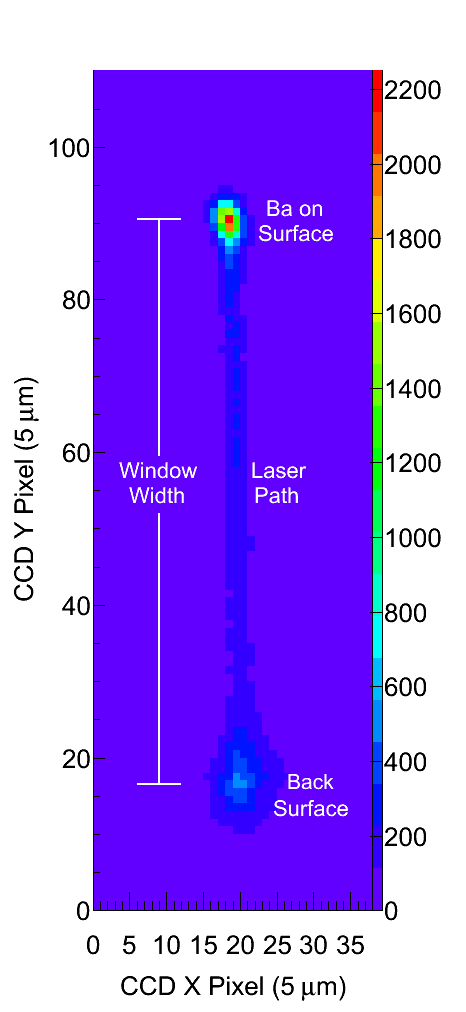
\includegraphics[width=.4\textwidth]{figures/imageExamp.png}
                \caption{Example image of a Ba\textsuperscript{+} deposit on a c-plane sapphire window of 0.5~mm thickness excited by a focused laser, using a 620-nm fluorescence band-pass filter.}
\label{fig:imageexamp}
\end{figure}

An example raw image of the focused 570~nm dye laser on a Ba\textsuperscript{+} deposit using the fluorescence of the 619-nm peak is shown in Fig. \ref{fig:imageexamp}.  With 4$\times$ magnification, each pixel corresponds to 5~$\mu$m$\times$5~$\mu$m on the window.  The laser's path through the window is faintly visible by the residual broad Cr\textsuperscript{3+} fluorescence that is passed by the 620-nm band-pass filter.  The laser is focused at the top surface of the window, which faces the ion beam.  The surface background is seen on the back surface, and the 619-nm Ba fluorescence stands out above both backgrounds on the top surface.  The imaging resolution results in a 1/e$^{2}$ radius of about 12~$\mu$m when imaging the 2.06~$\mu$m $\times$ 2.66~$\mu$m 1/e$^{2}$ laser spot.

\section{Wavelength Calibration}

Wavelength calibration of the spectrometer was done using three lasers whose wavelengths were first measured with a Burleigh Wavemeter:  a red diode laser at 656.99~nm, a doubled Nd:YAG laser at 532.23~nm, and the C480 blue dye laser typically around 475~nm.  These lasers were directed at the same position on the sapphire window, and their scatter was imaged along the same path as the Ba fluorescence.  The WinSpec software applies the diffraction grating equation to calibrate each CCD pixel to a wavelength.

\section{Vibrations and Effective Laser Region}
\label{sec:vibes}

\begin{figure} %[H]
        \centering
                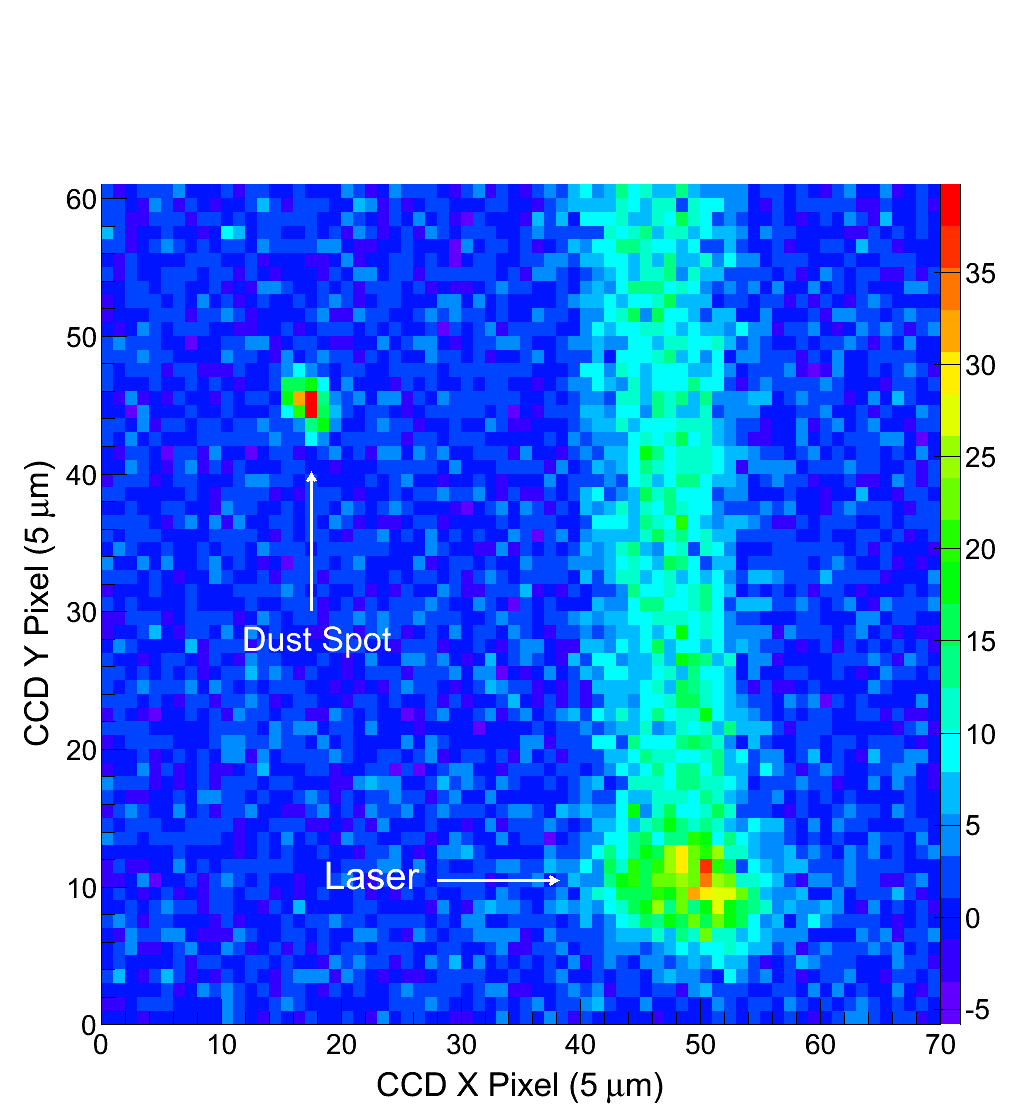
\includegraphics[width=.6\textwidth]{figures/image_dustspot.png}
                \caption{Example image of dust spot and laser during observation of cryostat vibrations.}
\label{fig:dustspot}
\end{figure}

\begin{figure} %[H]
        \centering
                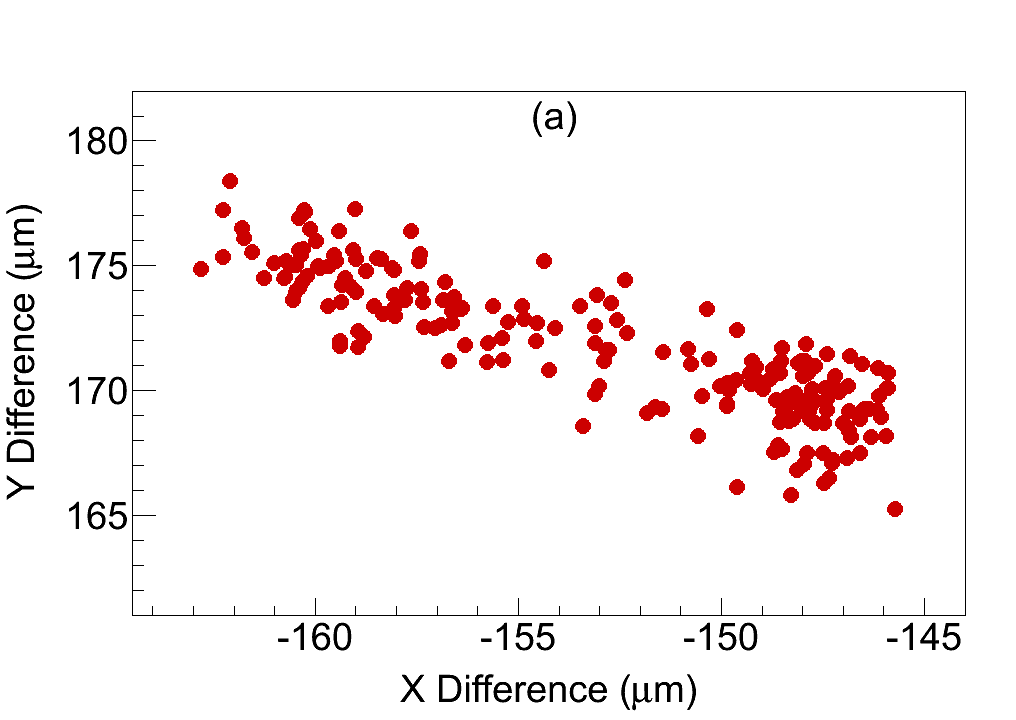
\includegraphics[width=.5\textwidth]{figures/cryovibes_a.png}
                ~
                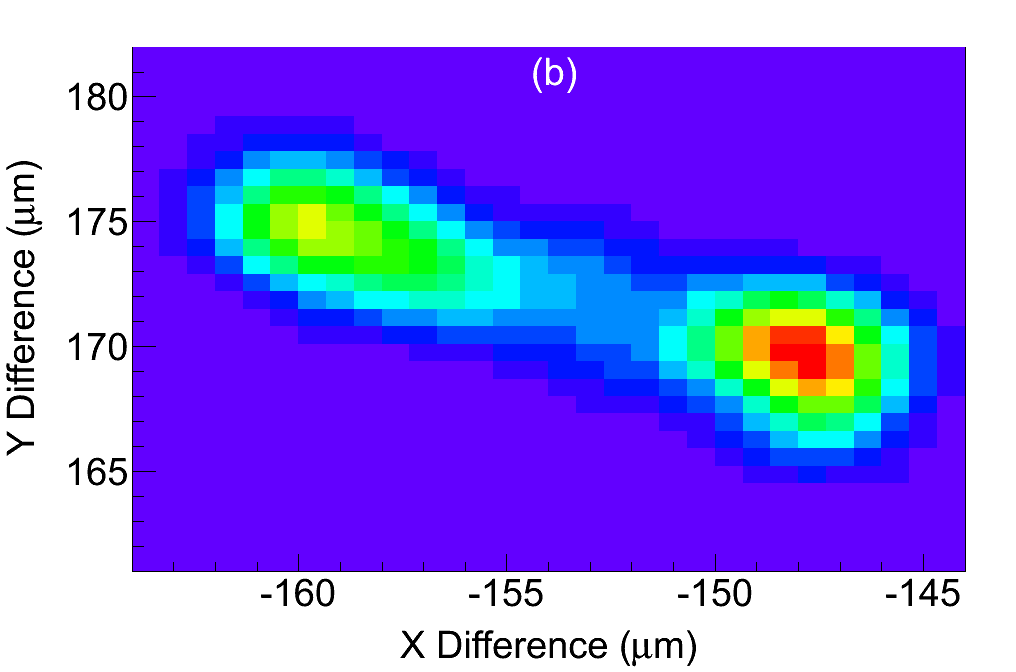
\includegraphics[width=.5\textwidth]{figures/cryovibes_b.png}
                \caption{Cryostat vibration measurements based on relative position of dust spot vs. laser on sapphire window in 50-ms snapshots (a), with 2D Gaussians of w$_{\text{x}} \times $w$_{\text{y}}$ = $2.06~\mu$m$ \times 2.66~\mu$m overlain on each point to represent total laser exposure vs. position (b).}
\label{fig:cryovibe2D}
\end{figure}

Relative vibrations between the laser and the sapphire window could occur on the micron scale from a few sources.  First, the laser is on a separate optical table from the cryostat and collection optics.  Second, the cryostat vibrates due to its He pump cycles.  Vibrations increase the total number of Ba atoms exposed during a measurement, but not the instantaneous number of Ba atoms in the laser beam area.

Vibrations were observed by determining the position of a ``dust spot" (a highly scattering feature on one sapphire window) relative to the position of the laser in an image on time scales down to 50~ms.  An example of an image from this experiment is shown in Fig. \ref{fig:dustspot}.  The dust spot was illuminated by a defocused 657~nm diode laser, and the 570-nm dye laser was somewhat defocused in order to optimally defocus the red laser with the same focusing lens. For each frame, 2D Gaussian functions with variable widths and magnitudes were fit to locate the center of the laser spot and the dust spot in order to measure their relative position.  The fit range for the laser spot was restricted in y so that it was not affected by the bulk sapphire fluorescence path.  The distances in x and y between the dust spot and laser are plotted for each 50-ms snapshot in Fig. \ref{fig:cryovibe2D}(a).  The distribution shows a correlation between x and y, indicating vibration in a particular direction.  The amplitude of the vibration is about 15~$\mu$m from this data.

To calculate an effective laser area with this vibration, each difference (x,y) between laser and dust spot was used as the center of a 2D Gaussian, each with w$_{x} = 2.06~\mu$m and w$_{y} = 2.66~\mu$m to represent the laser spot.  Such Gaussian functions were summed for all points to produce a distribution of summed laser exposure, shown in Fig. \ref{fig:cryovibe2D}(b).  The area enclosed by a 1/e contour then is a measure of the effective total exposed area.  On the other hand, signal at a given moment is still emitted only from the instantaneous laser area.  Then there are two possible definitions for the number of ions in the laser region, that provides the upper limit on the number of atoms.  In the absence of signal bleaching, the instantaneous number of atoms exposed is a reasonable definition for the number of atoms observed.  If there is large bleaching, the more conservative estimate is more appropriate.  Note that the factor between instantaneous and total exposure areas depends on the laser spot size.  The factor is about 4.7 for w$_{\text{x}} \times $w$_{\text{y}}$ = $2.06~\mu$m$ \times 2.66~\mu$m (astigmatism compensation and aspherical lens), and about 3 for w$_{\text{x}} \times $w$_{\text{y}}$ = $5~\mu$m$ \times 5~\mu$m (biconvex lens).

%In the absence of signal bleaching, the average number of atoms exposed is a good definition for the number of atoms observed.

%Since x and y movement are correlated, and since the movement is sinusoidal, the effective area is only about 5$\times$ the real laser spot size, and the effective laser region is about 40~$\mu$m$^{2}$.

%The difference between dust spot and laser positions is plotted in {\color{red}Fig. [fig vibe vs. time with sine fit]} for both x and y.  Each exposure in this plot is 50~ms, though readout time and camera shutter compensation time result in x~s between frames.  The best fit of a sine function results in a vibration frequency of x~Hz.  This is consistent with the audible frequency of the cryostat He pump.
%...could do this for rotated

For imaging of single Ba atoms, the relative vibration is the measure of most concern.  The vibration of the laser itself was seen to be small in this study.  Vibration of the collection optics will affect the imaging resolution, but not the number of atoms being observed, or the resolution of a single atom image in a laser raster scan.  These vibrations were minimized by stable mounting of the collection optics on large diameter posts.

%\vspace{10mm}

\begin{figure} %[H]
        \centering
                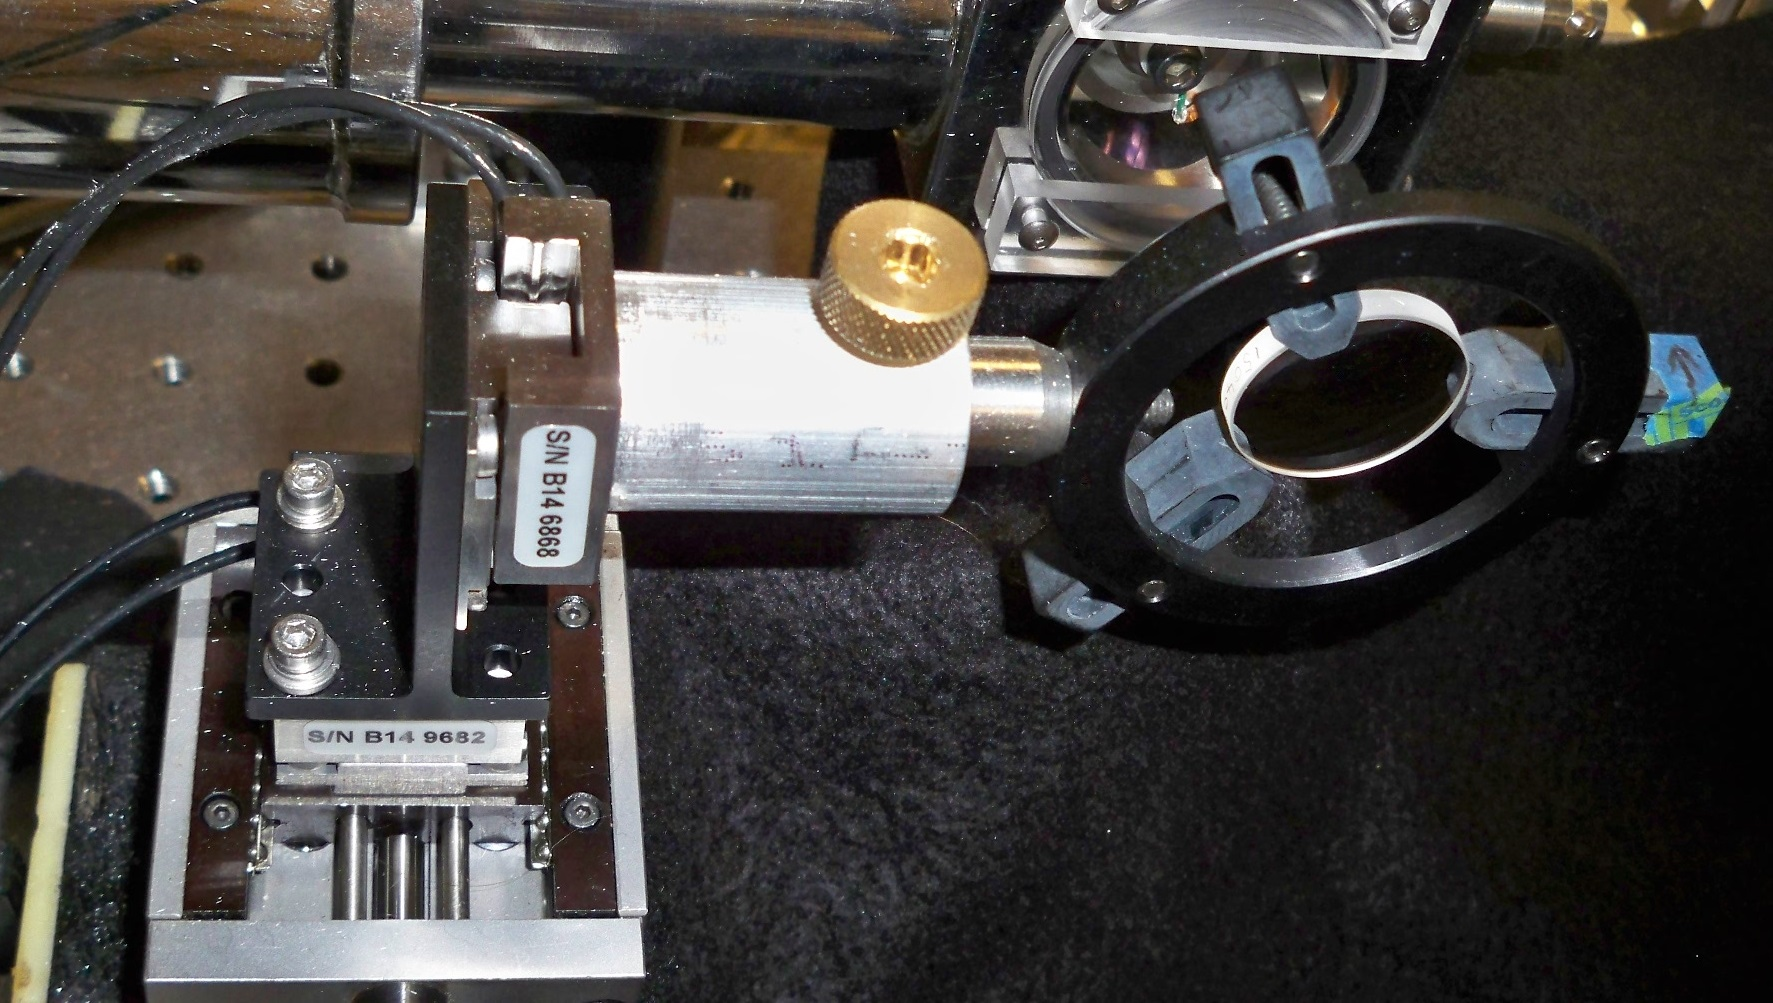
\includegraphics[width=.5\textwidth]{figures/stages_2.JPG}
                \caption{Asphere laser focusing lens mounted to two motorized Newport translation stages for laser scanning in x and y.}
\label{fig:laserStages}
\end{figure}


\section{Laser Scanning}
\label{sec:laserscanning}

In order to obtain images of separated single atoms, the laser focusing lens is attached to motorized translation stages which scan the laser position by translating the lens in x and y with sub-micron resolution, as shown in Fig. \ref{fig:laserStages}.  These stages sat atop a manual z-translation stage for laser focusing.  A LabVIEW program coordinates movement of these stages such that x or y position is stepped in between CCD frames, and each frame then corresponded to a position in a laser scan grid.

Relative laser-window vibration may be eliminated by using a different cryostat, or by gating the laser with a shutter to block exposure during He pump surges.  With no vibration, resolution of Ba atoms in scanned images is limited only by the size of the laser beam, not by the resolution of the collection optics and the CCD pixel size.

%\emph{\color{red}The stages used in this work were Newport AG-LS25, which are driven by piezoelectric motors, but without accurate position feedback.  As a result, some inconsistency in position reproducibility was observed.  The position of the focused laser, measured by the center of a 2D Gaussian fit to the image of the laser spot, is shown in Fig. [fig laser grid] for ... 2015-08-12 has one from chris where he did 2D gaus, but you should get that w/ them lined up from the start too, to separate init pos from inconsistency, and you need to quantify both}

%\emph{\color{gray}Show data on steps and reproducibility -- say this isn;t good and new stages will be used later.}
\chapter{Method}

The method of spectrum fitting is discussed in Sec. \ref{sec:fitting}, which is used in analysis for separating contributions of semi-resolved fluorescence peaks.  Background signals are discussed in Sec. \ref{sec:bgs} with the purpose of optimizing signal-to-background.

\section{Fitting of Spectra}
\label{sec:fitting}

In most circumstances, the different fluorescence peaks in a spectrum overlapped.  Thus it was necessary to fit the fluorescence spectra with a sum of peak-specific fit functions in order to extract peak heights and integrals.  These were used, e.g., in excitation spectra, annealing, and bleaching curves for different peaks.  Gaussians, Lorentzians and asymmetric functions were used, depending on the best match to a specific peak.

%The center and width parameters of the fit functions were fixed, while the amplitudes were the free fitting parameters.  Center and width parameters for each peak were determined by fitting spectra where that peak is relatively large.  Some fine-tuning was done to match slightly different shapes resulting from different excitation wavelengths.

\subsection{Fitting Spectra with Green Excitation}
\label{subsec:fitgrn}

\begin{figure} %[H]
        \centering
                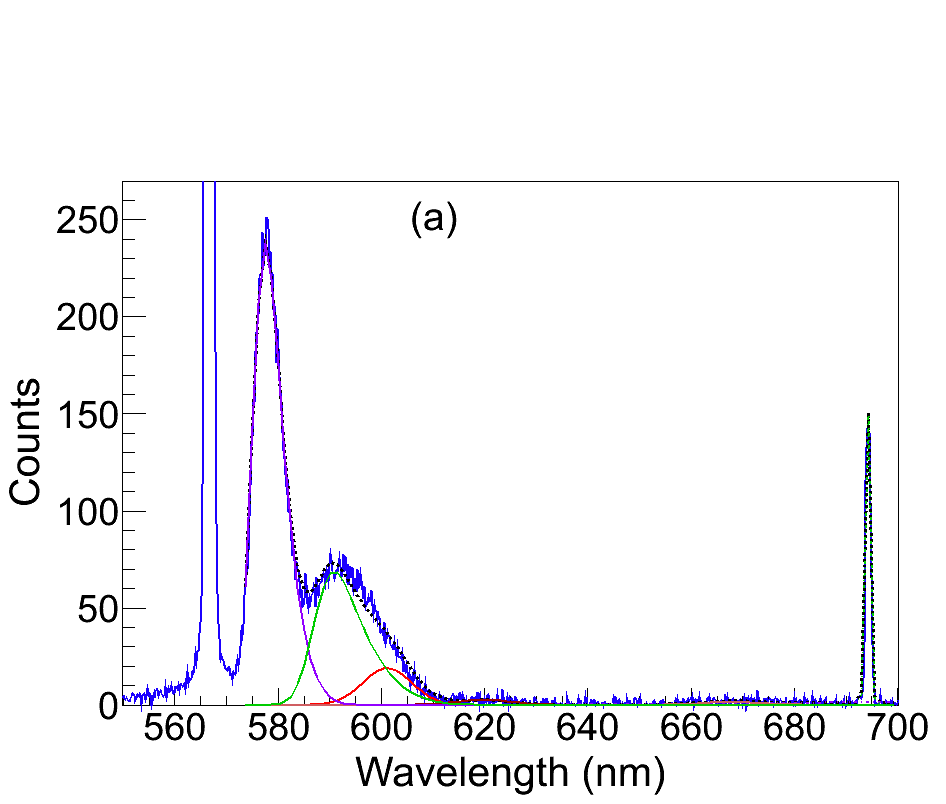
\includegraphics[width=.5\textwidth]{figures/spectra_fit_a.png}
                ~
                \includegraphics[width=.5\textwidth]{figures/spectra_fit_b.png}
                \includegraphics[width=.5\textwidth]{figures/spectra_fit_c.png}
                ~
                \includegraphics[width=.5\textwidth]{figures/spectra_fit_d.png}
                \includegraphics[width=.5\textwidth]{figures/spectra_fit_e.png}
                ~
                \includegraphics[width=.5\textwidth]{figures/spectra_fit_f.png}
                \caption{Example fits to spectra of Ba\textsuperscript{+} deposits with green excitation at (a) 566.6~nm, (b) 563.4~nm, (c) 546.3~nm, (d) 561.0~nm, (e) 555.9~nm, and (f) 567.3~nm.  Laser scatter can be seen in the lower wavelengths for some figures, especially in (a) where it is on the edge of the Raman filter cutoff.}
\label{fig:specFitsGrn}
\end{figure}

Example fits to spectra of Ba\textsuperscript{+} deposits for several different green excitation wavelengths are shown in Fig. \ref{fig:specFitsGrn}.  To incorporate the tail in the shape of the 577- and 591-nm peaks, an asymmetric function of the form $A(1+$erf$(\frac{x-a}{\sigma_{1}})(1-$erf$(\frac{x-a}{\sigma_{2}}))$ was used, where $a$ is the fixed center-defining parameter, $\sigma_{1}$ and $\sigma_{2}$ are fixed left and right width parameters, and $A$ is the free amplitude parameter.  The function erf() is an error function.  The 570-, 601-, 619-, and 670-nm peaks were fit with Gaussian functions with fixed widths ($\sigma$) of 1.7~nm, 4.7~nm, 5.3~nm, and 6.7~nm, respectively.  Rather than attempting frame-by-frame background subtractions, additional Gaussians were fit to the broad and sharp background fluorescence.  Two broad Gaussians centered at around 590~nm and 702~nm, and one sharp Gaussian at 694~nm, were chosen by fitting spectra of Xe-only deposits.  These backgrounds and their excitation spectra are discussed in \ref{sec:bgs}.  The full fit, i.e. the sum of each contributing peak fit, is the dotted black line.  Though the shapes do not match perfectly for all excitation wavelengths, the fits still follow the peak amplitudes well.  Ba emission and excitation spectra results are discussed in Sec. \ref{sec:fluorescence}.

\subsection{Fitting Spectra with Blue Excitation}
\label{subsec:fitblu}

Example fits to spectra of Ba\textsuperscript{+} deposits for several different blue excitation wavelengths are shown in Fig. \ref{fig:specFitsBlu}.  Gaussian functions were used for 532-, 568-, and 575-nm peaks with standard deviations ($\sigma$) of 2.4~nm, 5.0~nm, and 0.7~nm, respectively.  Lorentzian functions were used for the 553-, 592-, 635-, and 669-nm peaks with half width at half maxima ($\gamma$) of 1.7~nm, 13.8~nm, 10.4~nm. and 9.1~nm, respectively.  Similar to spectra with green excitation, the background components were fit with two broad Gaussians centered at 546.0~nm and 703.3~nm, with respective $\sigma$ of 49.0~nm and 30.5~nm, as well as one sharp Gaussian centered at 693.4~nm peak with $\sigma$ of 0.5~nm.  The fits around 478~nm (e.g., (c)) are not quite right, mainly due to a shift in central value of the 592-nm peak.  However, fit values still follow respective peaks heights well.  The 522- and 575-nm peaks are seen in (c), though the 522-nm peak is left out of the fitting range since it sits on the edge of the Raman filter cutoff.   These spectra are discussed in Sec. \ref{sec:BaPlus}.

\begin{figure} %[H]
        \centering
                \includegraphics[width=.5\textwidth]{figures/spectra_blu_fit_a.png}
                ~
                \includegraphics[width=.5\textwidth]{figures/spectra_blu_fit_b.png}
                \includegraphics[width=.5\textwidth]{figures/spectra_blu_fit_c.png}
                ~
                \includegraphics[width=.5\textwidth]{figures/spectra_blu_fit_d.png}
                \caption{Example fits to spectra of Ba\textsuperscript{+} deposits with blue excitation at (a) 461.7~nm, (b) 468.2~nm, (c) 478.3~nm, and (d) 488.2~nm.}
\label{fig:specFitsBlu}
\end{figure}

%\emph{results section, moved here: The broad blue BG ... what does its excitspec look like? is it possible it is the surface BG? ... anyway you need to mention it.  You need to figure what happened to the BG strangeness.}

%another sprectrum showing partial 601 nm is 20141107 run95.91 (547.0 nm excit.)

%i think you can leave this out: Curves in (a) have about 100$\times$ the laser power used in the excitation spectrum (e.g. (b)) where low intensity is desired to avoid bleaching during the scan.  

%A 566~nm Raman filter was used to attenuate the majority of the laser scatter, however the small amount of scatter passed by the filter was used to determine the frame's excitation wavelength.  Each peak's fit contribution was then integrated and scaled by the frame's laser power, as the power output is not constant through the dye range.

\section{Background Spectra}
\label{sec:bgs}

\begin{figure} %[H]
        \centering
                \includegraphics[width=.5\textwidth]{figures/Cr_a.png}
                ~
                \includegraphics[width=.5\textwidth]{figures/Cr_b.png}
                \caption{(a) Sapphire bulk emission with 562-nm excitation at 11~K, and (b) excitation spectrum of the sharp 694-nm emission peak using three different laser dyes.  Due to different laser powers and exposure times, the R110 and R6G were scaled to match at their boundary.}
\label{fig:Cr}
\end{figure}

\begin{figure} %[H]
        \centering
                \includegraphics[width=.7\textwidth]{figures/Cr_broad.png}
                \caption{Excitation spectra for weaker sapphire bulk emissions (blue,orange) along with that of the strong 694-nm emission (red) at 11~K.}
        \label{fig:CrBroad}
\end{figure}

The sharp and broad background discussed in Sec. \ref{subsec:fitgrn} is mainly due to Cr\textsuperscript{3+} impurity ions in the sapphire window.  A spectrum of this fluorescence with 562~nm excitation is shown in Fig. \ref{fig:Cr}(a).  The strong, sharp peak at 694~nm is a well-known $^{2}E$ - $^{4}A_{2}$ emission in the $d^{3}$ configuration of Cr\textsuperscript{3+} impurities in the sapphire bulk \cite{SapphireRlines1964,SapphireRlines2010}.  An excitation spectrum for this peak is shown in Fig. \ref{fig:Cr}(b) over the range all three dyes R6G, R110, and C480, using one of the sapphire windows with higher Cr\textsuperscript{3+} content.  Multiple features are observed in the excitation spectrum, obtained by integrating the 694-nm peak fit (Sec. \ref{sec:fitting}) vs. excitation wavelength.  The broad absorption in the green/yellow, peaking around 550~nm, with vibrational peaks on the red tail, agree with well understood features in the spectrum of Cr\textsuperscript{3+} in sapphire at 77~K, including three sharp peaks in the blue at 468.4, 474.8, and 476.5~nm \cite{SapphireFord,SapphireMcclure}.  In addition to the 694-nm peak, a weaker and much broader emission is observed, along with three weak peaks in the 615-635~nm region.  Excitation spectra for these fluorescence components are shown in Fig. \ref{fig:CrBroad} for the R6G dye range.  In this experiment, the laser was de-focused to about w = 200~$\mu$m, and the emission observed had contribution of the surface background as well as the bulk sapphire emission.  This is negligible for the prominent 694-nm peak, however the rising features of the surface background emission, near 600~nm and 567~nm, can be seen in the excitation spectra of the weaker components (blue, and especially orange curves in Fig. \ref{fig:CrBroad}).  Nonetheless, observation of the same vibrational peaks as in the 694-nm peak excitation spectrum demonstrates that the broad emission and weak peaks in the 620 band-pass (Fig. \ref{fig:Cr}(a)) are also due to Cr\textsuperscript{3+} in the sapphire.  Commercially available c-plane quality sapphire windows contain low concentrations of Cr\textsuperscript{3+}.  Sample windows of 0.75" diameter and 0.02" thickness from a few companies were tested, and those from Meller Optics produced the lowest sapphire bulk emission in the 620-nm band-pass region.

An additional background emission was observed from the surfaces of the window.  Its broad fluorescence is shown in Fig. \ref{fig:surfBG}(a) with a 610-nm Raman filter cutoff and 570.4~nm excitation, and its excitation spectrum is shown in Fig. \ref{fig:surfBG}(b) over the R6G dye range.  The nature of this emission has not been determined, however a few features were identified.  One was that the emission increased as the window temperature was decreased, down to about 100~K where it remained flat down to 11~K, shown in Fig. \ref{fig:BGtempDependence}.  Another feature of the surface background is that it bleaches with laser exposure.  In order to reduce this background in imaging experiments, as well as to reduce run-to-run variation in the background due to bleaching, the sapphire window was pre-bleached for at least half an hour.  Decay of the surface background emission, with intermittent observation during a pre-bleaching process, is shown in Fig. \ref{fig:surfBGbleach}.  For efficient pre-bleaching, the dye laser tuned to 580.5~nm for higher laser power, though the observation points in Fig. \ref{fig:surfBGbleach} are taken with the dye laser at 570~nm with the same laser power used in the following Ba imaging experiment.  During imaging experiments, frequent Xe-only deposits were made in order to track surface background emission to establish proper background subtraction.

\begin{figure} %[H]
        \centering
                \includegraphics[width=.5\textwidth]{figures/surfaceBG_a.png}
                ~
                \includegraphics[width=.5\textwidth]{figures/surfaceBG_b.png}
                \caption{(a) Surface background emission spectrum w/ excitation at 570.5~nm, and (b) excitation spectrum through wavelengths in R6G dye range.  The sharp drop in (a) around 608~nm is the Raman filter cutoff.}
\label{fig:surfBG}
\end{figure}

%\begin{figure} %[H]
%        \centering
%                \includegraphics[width=.4\textwidth]{figures/xe_variation.png}
%                \caption{Background counts in focused laser region over the course of an experiment.}
%\label{fig:xevar}
%\end{figure}

%\emph{\color{gray}from results} Variation in the background level, dominated by the surface background, is shown in Fig. \ref{fig:xevar}.  Variation was most likely caused by drift of the laser position on the window, to regions of different historical bleaching.  Local variations are at the single-atom signal level, however positive signal after subtraction, even at the single-atom level, demonstrates that this variation is sufficiently low.

%Spacial variation in the background is especially cumbersome in a laser scanning experiment, as discussed in \ref{sec:scanning}. 

%speculation:    Given these behaviors, it is possible that the surface background is caused by a species which freezes to the window, or something which coats the window and fluoresces more at lower temperatures.  In either case, the bleaching could be explained by evaporation with laser heating, or by optical pumping of the species into a metastable state.

\begin{figure} %[H]
        \centering
                \includegraphics[width=.6\textwidth]{figures/bg_temp_dep.png}
                \caption{Temperature dependence of surface (red) and sapphire bulk (b) backgrounds.}
\label{fig:BGtempDependence}
\end{figure}

\begin{figure} %[H]
        \centering
                \includegraphics[width=.4\textwidth]{figures/Bleach_SurfaceBG_20150807_part1.png}
                \caption{Decay of surface background emission during pre-bleaching of the sapphire window.}
\label{fig:surfBGbleach}
\end{figure}

\begin{figure} %[H]
        \centering
                \includegraphics[width=.7\textwidth]{figures/S_to_B_both.png}
                \caption{Optimization of signal to background with the 619-nm fluorescence signal (S) for emission from the surface background (B$_{\text{surf}}$, red) and for the bulk sapphire emission (B$_{\text{sap}}$, cyan).}
        \label{fig:StoB}
\end{figure}

Consideration of signal-to-background ($S$/$\sqrt{B}$) guided the choice of 570~nm for excitation of the 619-nm fluorescence.  $S$/$\sqrt{B}$ for emission passed by the 620-nm band-pass filter is plotted vs. excitation wavelength in Fig. \ref{fig:StoB} for the surface background (B$_{\text{surf}}$) as well as for the sapphire bulk emission (B$_{\text{sap}}$).  The peak in $S$/$\sqrt{B}$ represents the optimal excitation wavelength respective to each of the two background sources.  Around 568.5~nm is optimal vs. the sapphire emission, and around 571~nm is optimal vs. the surface background emission. 570~nm, which was used in sensitive imaging experiments, is nearly optimal in both cases, although the bulk sapphire background contribution was small in in these experiments.

%Consideration of signal-to-background ($S$/$\sqrt{B}$) guided the choice of 570~nm for excitation of the 619-nm fluorescence.  $S$/$\sqrt{B}$ is plotted vs. excitation wavelength in Fig. \ref{fig:StoB} for the surface background (B$_{\text{surf}}$) as well as for combination of the surface background and sapphire bulk emission (B$_{\text{sap + surf}}$).

%The Cr\textsuperscript{3+} emission has an inverse relationship with temperature, shown in Fig. \ref{fig:BGtempDependence}.

%with Cr\textsuperscript{3+} concentrations of around {\color{red}10 ppt} observed.

%(peaks around? May need to ask Bill about what peaks exist and at what temps ... a new idea is to just leave it vague, as ``peaks" since you're sure there are at least 2, but vauge is OK)

\chapter{Results: Spectroscopy}
\label{chapter:spectroscopy}

The spectroscopy of Ba in SXe was studied in detail beyond that reported in two previous theses \cite{Shon,Brian}, with the goal of imaging single Ba atoms.  Emission and excitation spectra are analyzed in Sec. \ref{sec:fluorescence}, with particular interest in the 619-nm peak in Sec. \ref{sec:619identification}.  Studies of temperature and bleaching effects in Sections \ref{sec:tempanneal} and \ref{sec:bleaching} aid in determining optimal conditions for observation.  Finally, candidate emission lines for Ba\textsuperscript{+} in SXe are discussed in Sec. \ref{sec:BaPlus}.

%Backgrounds are analyzed in \ref{sec:bgs} in order to optimize sensitivity,

\section{Excitation and Emission of Ba in SXe}
\label{sec:fluorescence}

Deposits of Ba in SXe absorb primarily between 540~nm and 570~nm.  An absorption spectrum, obtained by observing absorption of white light by a large Ba deposit at 10~K, is shown in Fig. \ref{fig:BaAbs}.  Significant broadening, as well as a 4-nm redshift  of the central peak, occur relative to the vacuum $6s^{2}$ $^{1}$S$_{0} \rightarrow 6s6p$ $^{1}$P$_{1}$ absorption value of 553.5~nm.  Initial absorption and emission spectra was done with the Ba getter source \cite{Mong2015,Shon,Brian}, which is expected to produce neutral Ba with minimal Ba\textsuperscript{+}.  The emission spectrum in Fig. \ref{fig:BaAbs} was obtained by 557-nm excitation of a Ba\textsuperscript{+} deposit, made at 45~K and observed at 11~K.  Observation of the same 577- and 591-nm fluorescence peaks from Ba getter deposits demonstrates that these peaks are emission of neutral Ba.  Therefore some neutralization of the ions takes place during the deposit \cite{Mong2015,Shon,Brian}.  The fraction of ions neutralized has not yet been determined.

\begin{figure} %[H]
        \centering
                \includegraphics[width=.7\textwidth]{figures/BaAbs_fromBaSpec.png}
                \caption{Absorption and emission spectra of neutral Ba in SXe.  The absorption is of a Ba getter deposit at 10~K, and the emission is of a (neutralized) Ba\textsuperscript{+} deposit, deposited at 45~K and observed at 11~K with 557~nm excitation.  From \cite{Mong2015}.}
\label{fig:BaAbs}
\end{figure}

\begin{figure} %[H]
        \centering
                \includegraphics[width=.8\textwidth]{figures/excitspec_grn_spectra_v3.png}
                \includegraphics[width=.8\textwidth]{figures/excitspec_grn.png}
                \caption{(a) Fluorescence spectra for a few different excitation wavelengths, and (b) excitation spectra for all observed Ba fluorescence peaks.  Exposures are 1~s.}
\label{fig:excitspecGrn}
\end{figure}

%(relative magnitudes are arbitrary as they are affected by relative site populations and fluorescence efficiencies)

%Put legend in (b)? It's crowded.

%\begin{equation}
%A(1+erf(\frac{x-a}{\sigma_{1}})(1-erf(\frac{x-a}{\sigma_{2}}))
%\label{eqn:specfit}
%\end{equation}

%Deposition at temperatures higher than 10~K and exploration of more excitation wavelengths have led to discovery of emission peaks beyond the 591- and 577-nm peaks reported in \cite{Shon} and \cite{Brian}.  

Emission spectra, scaled by laser power, of a Ba\textsuperscript{+} deposit made at 44~K and observed at 11~K are shown in Fig. \ref{fig:excitspecGrn}(a) for a few different excitation wavelengths.  The 577- and 591-nm peaks are clear at all three wavelengths, with varying strength.  Peaks at 570~nm and 601~nm, first reported here, are both clear at 546-nm excitation.  The 619-nm peak is stronger at higher wavelength, and the 670-nm peak is clear at 556-nm excitation.

Excitation spectra, shown in Fig. \ref{fig:excitspecGrn}(b), were produced by scanning the dye laser and measuring the magnitude of each fluorescence peak vs. excitation wavelength.  For each frame, the spectrum was fit with a sum of peak-specific fit functions, where function shape parameters were fixed (centers and widths) and magnitudes were allowed to float.  Fitting is described in Section \ref{subsec:fitgrn}.  Since the dye laser power varies over the tuning range, fluorescence counts at each excitation wavelength are scaled to the laser power in that frame.  Since signal levels are dependent on the deposit size, the absolute scale is arbitrary.  Thus, curves were scaled for visibility on the same plot.  The discontinuity around 566~nm for the 619- and 670-nm peaks is the boundary between the scan range of different laser dyes.  R6G dye was used for higher wavelengths and R110 for lower wavelengths.  Bleaching, discussed in Sec. \ref{sec:bleaching}, was prevented from occurring in the 570-, 577-, 591-, and 601-nm peaks during excitation spectrum scans by using low laser intensities.  For those peaks, maximal laser power was 0.1~mW, and the laser radius was w = 7~mm with no focusing.  The scans for the 619- and 670-nm peaks, which bleach only at much higher intensities, were done with the laser somewhat focused to radii of w = 1000~$\mu$m in the R110 dye range, and w = 200~$\mu$m in the R6G dye range, with maximal laser powers of 10~mW and 100~mW, respectively.

%Due to these different laser radii, as well as different deposit sizes, curves for the R6G segments (619- and 670-nm peaks) required special scaling to line up with their respective R110 segments.  This scaling was slightly different between the 619- and 670-nm peaks, likely due to different relative populations of those sites on the different deposits.

%INFO:  619- and 670-nm deposits had 5 s DC, with 24 nA on R110 one and 41.5 nA on R6G one

\section{619-nm Peak Attribution}
\label{sec:619identification}

\begin{figure} %[H]
        \centering
                \includegraphics[width=.5\textwidth]{figures/Ar_vs_Ba.png}
                ~
                \includegraphics[width=.5\textwidth]{figures/ArImaging.png}
                \caption{Comparison of signal observed for deposits with the Ba\textsuperscript{+} ion beam (red), Ba getter (blue), and Ar\textsuperscript{+} ion beam (green) (a), and signal through 620-nm band-pass from deposits of small to large numbers of Ar\textsuperscript{+} ions in SXe.}
\label{fig:ArVsBa}
\end{figure}

The 619-nm peak, as well as the 670-nm peak, was demonstrated to be related to neutral Ba by a few further tests.  The spectra of a large Ba\textsuperscript{+} deposit and a deposit made with the Ba getter are compared in Fig. \ref{fig:ArVsBa}(a).  The 619-nm and 670-nm peaks are observed with both sources with similar shapes.  Since the getter produces only neutral Ba, these peaks are attributed to neutralized Ba\textsuperscript{+} ions.  Observation of a deposit of Ar\textsuperscript{+} of similar energy and charge in SXe is also shown in Fig. \ref{fig:ArVsBa}(a).  The lack of fluorescence in the Ar\textsuperscript{+} deposit eliminates a matrix-damage-related source of the fluorescence, such as color centers.  Imaging experiments of Ar\textsuperscript{+} deposits were also performed, with both pulsing and continuous ion beams.  Summed counts/mW from these deposits are shown to be consistent with background in Fig. \ref{fig:ArVsBa}(b).  To be similar to Ba imaging experiments discussed in Sec. \ref{sec:imaging619}, the focused dye laser was at 570~nm, and a 620-nm band-pass filter was used on the fluorescence.

%Finally, to rule out the possibility that the signal in Ba imaging experiments is due to passed wavelengths far from the 620-nm band-pass region, e.g. infrared, imaging experiments of Ar\textsuperscript{+} deposits in SXe were performed with both pulsing and continuous ion beams.  The same 620-nm band-pass filter was used, as well as the same focused 570-nm laser, to be similar to Ba\textsuperscript{+} 619-nm imaging experiments.  Summed counts from these deposits were consistent with background, as shown in Fig. \ref{fig:ArVsBa}(b).

%Observation of the fluorescence with two different types of Ba sources is itself positive.  In addition, observation of the fluorescence with the low deposit energy of the getter may bode well for the prospect of grabbing on a probe in LXe.

%at one point youthought leak rate dependence could go here

\section{Annealing/Temperature Dependence}
\label{sec:tempanneal}

%\emph{\color{gray}When does it need to be mentioned that certain data was also used in the paper(s)?}

%Matrix site occupancies for Ba atoms

\begin{figure} %[H]
        \centering
                \includegraphics[width=.7\textwidth]{figures/spectra_temperature_conditions.png}
                \caption{Spectra of peaks around 590~nm of a Ba\textsuperscript{+} deposit made at 11~K before and after annealing to 39.4~K, and one made at 44~K.  All observations are at 11~K.  Both Ba\textsuperscript{+} deposits are 15~s, however the 44~K deposit is scaled slightly to account for different ion current.  Laser power was about 0.1~mW with an unfocused beam radius of w = 7.056~mm, at 566~nm wavelength.}
\label{fig:specTempConditions}
\end{figure}

\begin{figure} [h]
        \centering
                \includegraphics[width=.8\textwidth]{figures/619_deposit_temp.png}
                \caption{Images of 619-nm fluorescence in focused 570-nm laser region for deposits made at (a) 11K and (b) 52~K.  Deposits are 3~s of continuous Ba\textsuperscript{+} current.  Exposures are 0.1~s.  Observation is at 11~K.}
\label{fig:specTempConditions619}
\end{figure}

Emission spectra can depend on the thermal history of the deposit, such as the temperature at which it was made, and any annealing of the deposit.  Spectra observed at 11~K with different thermal histories are shown in Fig. \ref{fig:specTempConditions}.  Peak shapes in the annealed deposit look similar to those in the deposit made at 44~K.  However, larger signal is observed in the deposit at 44~K.  The broader emission around 596~nm in non-annealed 11-K deposits may be due to a higher population of the 601-nm peak,which is not resolved from the 591-nm peak.  The deposit temperature dependence of the 619-nm peak is illustrated by images comparing the fluorescence from a focused laser through the 620-nm band-pass filter, shown in Fig. \ref{fig:specTempConditions619}.  The level of 619-nm signal is about 3$\times$ larger in deposits made at 52~K vs. 11~K.  Imaging is described in detail in Chapter \ref{chapter:imaging}.  These tests guided the standard of depositing at 50$\pm$5~K when observing the 577-, 591-, and/or 619-nm peaks.

%differences in the relative amplitudes of the peaks could be due to differences in matrix site populations

%the respective 31~nm/s and 37~nm/s are from the same Xe leak rate, resulting in different SXe deposition rates daccording to Fig. \ref{fig:fringes_52K_vs_11K}

%A study of deposit conditions for the 619-nm peak (rather than just temp-depend)

% is discussed briefly in \ref{sec:bleaching}.

%5.4E4 Xe:Ba for leak 48 50~K (31 nm/s)

% at leak setting 48 (619 vs temp)

\begin{figure} %[H]
        \centering
                \includegraphics[width=.7\textwidth]{figures/spectra_annealing.png}
                \caption{Spectra of a large Ba\textsuperscript{+} deposit through several annealing cycles.  The initial deposit was at 11~K.  The laser power was about 0.2~mW with an unfocused beam radius of w = 7.056~mm, at 564~nm wavelength.  \cite{Mong2015}}
\label{fig:specAnneal}
\end{figure}
%These are selections from the full data set shown as peak counts vs. temperature in Fig. \ref{fig:annealGrn}

\begin{figure} %[H]
        \centering
%                \includegraphics[width=.5\textwidth]{figures/spectra_anneal_fit.png}
%                ~
                \includegraphics[width=.5\textwidth]{figures/anneal_577peak_topspace.png}
                \includegraphics[width=.5\textwidth]{figures/anneal_591peak.png}
                ~
                \includegraphics[width=.5\textwidth]{figures/anneal_601peak.png}
                \includegraphics[width=.5\textwidth]{figures/anneal_619peak.png}
                ~
                \includegraphics[width=.5\textwidth]{figures/anneal_670peak.png}
                \caption{Fit peak counts for the (a) 577-, (b) 591-, (c) 601-, (d) 619-, and (e) 670-nm fluorescence peaks through three annealing cycles of the Ba\textsuperscript{+} deposit made at 11~K.  ``1", ``2", and ``3" mark the beginning of each anneal cycle.  The laser power was about 0.2~mW with an unfocused beam radius of w = 7.056~mm at 564~nm wavelength.}
\label{fig:annealGrn}
\end{figure}
%\clearpage weird

Fluorescence spectra with 564~nm excitation through several annealing cycles for a deposit made at 11~K are shown in Fig. \ref{fig:specAnneal}.  The initial exposure shows significant 591- and 601-nm (unresolved from one another) emission, with some 577-nm emission.  All peaks are reduced at the high temperature ends of the anneal cycles.  The return to lower temperatures results in an overall increase for some peaks, e.g. the 577- and 619-nm peaks, and an overall loss of others, e.g. the 670-nm peak.  

Fit peak counts (fitting is described in Sec. \ref{sec:fitting}) vs. temperature are shown in Fig. \ref{fig:annealGrn}.  The 577-nm and 619-nm peaks gained significantly with the first anneal, suggesting that they are due to more stable matrix sites.  Both of these peaks remained about the same after the second cycle (small gain in 577-nm), and both had loss after the third cycle, which reached the higher temperature of 48~K.  The 591-nm had moderate loss with each cycle.  The 601-nm peak had nearly complete loss in the first anneal cycle.  The 670-nm peak had significant loss, with more loss after each succeeding anneal cycle, each of which reached higher a temperature than the last.

%This could be due to greater diffusion at higher temperature leading to Ba/Ba interactions.

%At this wavelength, all observed Ba peaks are prominent except the 570-nm peak.

% In this interpretation, the 601-nm peak along with the 591-nm peak fit the broader peak in the initial 11~K deposit.

Aside from matrix site changes, direct temperature dependence of fluorescence can be observed in annealing cycles.  The 577-, 591- and 619-nm peaks have their highest amplitude at 11~K.  The 577-nm and 619-nm peaks reach a plateau at 11~K, while the 591-nm may benefit from even lower temperatures.  This suggests that a probe in nEXO may need to be extracted from the liquid chamber and moved to a separate evacuated chamber in order to cool to 11~K or below for most efficient observation.  

% After annealing, the 670-nm peak has its highest amplitude at around 25~K.

%\emph{\color{gray}601 and (not shown) 570 would require different wavelength to study.}

%[inverse relationship] could be due to a different matrix environment at higher temperature, or possibly a loss of fluorescence efficiency due to increased non-radiative decays from the excited state.  

%\vspace{40mm}
\section{Bleaching}
\label{sec:bleaching}

Decay of fluorescence with laser exposure, or bleaching, was observed for all six Ba fluorescence peaks.  Examples of bleaching spectra are shown in Fig. \ref{fig:specBleach}, with excitation at (a) 556.9~nm, (b) 562.6~nm, and (c) 566.3~nm, using a semi-focused laser of radius w = 1000 $\mu$m.  Each curve is the Ba emission spectrum at different points in time.  Bleaching is seen to be rapid for the 570-, 577-, 591-, and 601-nm peaks.  Negligible bleaching is observed for the 619- and 670-nm peaks in Fig. \ref{fig:specBleach}.  Nevertheless, even for these lines, some small bleaching was observed with the much higher intensity of a focused beam.

\begin{figure} %[H]
        \centering
                \includegraphics[width=.5\textwidth]{figures/bleach_spectra_a.png}
                \includegraphics[width=.5\textwidth]{figures/bleach_spectra_b.png}
                ~
                \includegraphics[width=.5\textwidth]{figures/bleach_spectra_c.png}
                \caption{Bleaching Ba emission peaks with excitation at (a) 556.9~nm, (b) 562.6~nm, and (c) 566.3~nm.  Laser power and exposure times are (a) 1.3~mW and 1~s, (b) 7.5~mW and 0.2~s, and (c) 5.8~mW and 0.2~s.  Every tenth exposure is shown, beginning with the second in the darkest blue, ending with the darkest red.  Each is a 5-s continuous Ba\textsuperscript{+} deposit at 45~K, observed at 11~K. \cite{Mong2015}}
\label{fig:specBleach}
\end{figure}

%To produce a well-known laser intensity, the laser was de-focused to a specific beam waist, and the image of 619-nm fluorescence (which defines the laser region due to its low bleaching) from a large Ba\textsuperscript{+} deposit was centered in the spectrometer slit and a y-pixel region of interest (ROI) with edges at 90\% of the maximal intensity.  Ba spectra over time are shown in Fig. \ref{fig:specBleach}(a,b,c) for excitation at (a) 556.9~nm, (b) 562.6~nm, and (c) 566.3~nm, where relative bleaching rates between peaks can be seen to depend on the excitation wavelength.

\subsection{Bleaching of the 577- and 591-nm Peaks}
\label{sec:bleach577and591}

\begin{figure} %[H]
        \centering
                \includegraphics[width=.5\textwidth]{figures/bleach_compareEmission577vs591_specificSigmas_a.png}
                \includegraphics[width=.5\textwidth]{figures/bleach_compareEmission577vs591_specificSigmas_b.png}
                ~
                \includegraphics[width=.5\textwidth]{figures/bleach_compareEmission577vs591_specificSigmas_c.png}
                \caption{Fluorescence vs. number of excitations for three orders of magnitude (a,b,c) in laser intensity, for the 577-nm (purple) and 591-nm (green) fluorescence peaks.  The deposits were continuous Ba\textsuperscript{+} at 45~K, observed at 11~K, and exposures were 0.2 or 2~s.}
\label{fig:bleach_577vs591}
\end{figure}

The integrated counts for different peaks in each spectrum were determined by fits to the spectra, as described in Sec. \ref{sec:fitting}.  Integrated counts vs. number of excitations ($W_{12} \times t$) are shows in Fig. \ref{fig:bleach_577vs591} for both the 577-nm (purple) and 591-nm (green) fluorescence peaks, with laser intensities varying by two orders of magnitude from about 0.3~mW/mm\textsuperscript{2} (a) to about 40~mW/mm\textsuperscript{2} (c).  Intensities for each run are listed in the legends.  The excitation wavelengths used were 566.3~nm for the 577-nm peak and 562.6~nm for the 591-nm peak.  Bleaching is more rapid in the 591-nm peak than the 577-nm peak when low intensity is used (a).  For medium (b) and high (c) intensity, bleaching rates are similar.  In order to calculate the excitation rate $W_{12}$ for each run according to Eq. \ref{eqn:w12}, the cross section $\sigma(\nu)$ was calculated using the integral of the corresponding excitation spectrum (Fig. \ref{fig:excitspecGrn}), as explained in Sec. \ref{sec:fluorEff}.
%(see Fig. \ref{fig:excitspecGrn} for the excitation spectrum)

\begin{figure} %[H]
        \centering
                \includegraphics[width=.5\textwidth]{figures/bleach_compareExcitations_specificSigmas_a.png}
                ~
                \includegraphics[width=.5\textwidth]{figures/bleach_compareExcitations_specificSigmas_b.png}
                \caption{Fluorescence vs. number of excitations with different excitation wavelengths for (a) the 477-nm peak, and (b) the 591-nm peak.  Deposits erre continuous Ba\textsuperscript{+} at 45~K, observed at 11~K.}
\label{fig:bleach_excitCompare}
\end{figure}

Comparisons of bleaching with different excitation wavelengths are shown in Fig. \ref{fig:bleach_excitCompare} for (a) the 577-nm peak, and (b) the 591-nm peak.  In the case of the 577-nm peak (a), the excitation wavelengths (566.3 and 556.9~nm) correspond to different peaks in the excitation spectrum (Fig. \ref{fig:excitspecGrn}).  Very different bleaching rates were observed.  In the case of the 591-nm peak (b), the excitation wavelengths (562.6 and 556.9~nm) correspond to neighboring peaks in the triplet structure of the excitation spectrum.  The bleaching rates are similar, with a somewhat faster rate for the 556.9-nm excitation, which had about 2$\times$ the intensity.

% as the 562.6-nm excitation

Ultimately, these studies suggested the usage of the 577-nm peak in imaging small numbers of atoms due to its lower bleaching rate, especially with excitation on the high-wavelength end of the range studied.  Imaging of Ba atoms using a combination of the 577- and 591-nm peaks with excitation at 566~nm, via a band-pass filter passing 573 - 599~nm FWHM, is discussed in Sec. \ref{sec:imaging590and577}.

\begin{figure} %[H]
        \centering
                \includegraphics[width=.5\textwidth]{figures/bleach_model_vacuum_w12t_a.png}
                \includegraphics[width=.5\textwidth]{figures/bleach_model_vacuum_w12t_b.png}
                ~
                \includegraphics[width=.5\textwidth]{figures/bleach_model_vacuum_w12t_c.png}
                \caption{Vacuum model (orange) comparisons to 591-nm fluorescence with excitation at (a) 562.6~nm, and (b) 566.3~nm.  Deposits were continuous Ba\textsuperscript{+} at 45~K, observed at 11~K.}
\label{fig:bleach_model_vac}
\end{figure}
%\color{gray}may want to show 3, though 1 I think was bad.

A numerical model of fluorescence vs. time for a 5-level system of Ba in vacuum, described in Sec. \ref{sec:model} and using the Ba vacuum transition parameters given in Table \ref{table:BaTransitions}, is compared to bleaching data of the 591-nm peak in Fig. \ref{fig:bleach_model_vac} for excitation at (a) 562.6~nm, and (b) 566.3~nm.  In the model, the input value for the excitation rate $W_{12}$ is similar to the calculated value based on the laser power, laser radius, and \emph{\color{gray}No} cross-section of Ba in SXe of $1.2 \times 10^{-15}$~cm\textsuperscript{2} measured in \cite{Brian}, with slight adjustments.  $W_{12}$ is scaled by 0.8 for 562.6-nm excitation (a), and 0.5 for 566.3-nm excitation, which is explained by the lower value in the 591-nm peak excitation spectrum at 566.3~nm.  Each model is normalized to the beginning of its respective data set.  Agreement between the model and data is observed for the first several seconds of the bleaching process, and then deviation occurs in two major regions, A and B.  In region A, the model predicts more rapid bleaching than is observed.  In region B, the model predicts a leveling off as a steady state in energy level populations is reached, though the data continues to decay beyond this region.

%The agreement between model and data in the initial rapid decay region suggests that a major contribution of bleaching is indeed optical pumping into the metastable D states \emph{\color{gray}Bill probably won't like that, so you might just sort of start with the next sentence with a sort of ``deviation from vacuum agreement" or something}.  Subsequent deviation from the vacuum model could be explained by altered transition rates in the SXe matrix.  Models with modified transition rates are shown in Fig. [].  [first solve A and then B]  ummm whaaaat i don't even know, whaaaat.  well:  you say, if you show the vacuum model, you should at least \emph{try} some alterations ... maybe you can come up with reasonable try type things if you can't get something good.

% look in model/matrix/fromVacuum/ and subsequent folders for where you are with model fixes

%talk about hole bleaching?

%\begin{figure} %[H]
 %       \centering
  %              \includegraphics[width=.9\textwidth]{figures/hole_bleach_590.png}
   %             \caption{}
%\label{fig:testfig}
%\end{figure}

\subsection{Re-pumping}

%mention that similarity to vacuum rates suggests laser repumping?

Re-pumping of optically pumped Ba could require up to three additional lasers, one for each of the populated metastable D states.  The optimal excitation wavelength for each transition would need to be discovered using tunable lasers in the infrared.  However, mixing of states and/or alterations in transition rates for Ba in the Xe matrix could lower the number of lasers needed.  Re-pumping was attempted, with low-cost and on-hand lasers, for the direct infrared transitions as well as the higher-level transitions shown in Fig. \ref{fig:elevsBa}.  A 1550-nm diode laser and a 1064-nm Nd:YAG laser were used to attempt direct re-pumping from the \textsuperscript{1}D and \textsuperscript{3}D states, respectively.  A 657-nm diode laser was used to attempt excitation from the \textsuperscript{3}D states into the higher-level $5d6p$ \textsuperscript{3}D$_{1}$\textsuperscript{o} state, similar to the red laser utilized in the Ba MOT in \cite{BaMOT} for the $6d5d$ \textsuperscript{3}D$_{1}$ state.  The blue C480 dye laser and 406-nm Kr ion laser were used to attempt excitation from the \textsuperscript{1}D state into the higher-level states $6s7p$ \textsuperscript{1}P$_{1}$\textsuperscript{o} and $6s8p$ \textsuperscript{1}P$_{1}$\textsuperscript{o}, respectively.

%MOT was with 659.7~nm I think

\begin{figure} %[H]
        \centering
                \includegraphics[width=.5\textwidth]{figures/bleach_re-pump_a.png}
                ~
                \includegraphics[width=.5\textwidth]{figures/bleach_re-pump_b.png}
                \caption{Bleaching data with and without additional re-pump lasers at (a) 1064~nm ($\sim$18~mW/mm\textsuperscript{2}), 1550~nm ($\sim$9~mW/mm\textsuperscript{2}), 657~nm ($\sim$9~mW/mm\textsuperscript{2}) and 472.64~nm ($\sim$14~mW/mm\textsuperscript{2}), and (b) 406~nm.  All curves have 1.4 - 1.5~mW of 555-nm excitation, semi-focused to around 600-$\mu$m beam radius.  Deposits are (a) 6~s and (b) 3~s continuous Ba\textsuperscript{+} at 11~K.}
\label{fig:bleach_repump}
\end{figure}

591-nm fluorescence counts vs. time for several Ba\textsuperscript{+} deposits made and observed at 11~K are shown in Fig. \ref{fig:bleach_repump} for several laser combinations, all of which were combined by dichroic filters into the same path.  Each curve is a separate deposit, all of which are scaled to begin at the same point for comparison.  In Fig. \ref{fig:bleach_repump}(a), green-only (555~nm) excitation (i.e., no re-pump lasers) is shown along with green + IR (1064~nm and 1550~nm), green + IR + red (657~nm), green + IR + blue (C480 dye at 472.64~nm), and green + IR + red + blue.  Increased bleaching was observed by inclusion of these re-pump lasers, especially with the blue laser.  In Fig. \ref{fig:bleach_repump}(b), green-only is shown again along with green + violet (Kr ion laser at 406~nm) at two different powers.  Increased bleaching was observed with the violet laser, with more bleaching at the higher violet laser power.

%The only effects observed on bleaching rates by these re-pump lasers were increased bleaching by the blue dye and 406-nm Kr ion lasers.  Some effect of a return of fluorescence was observed after separate exposures of low-intensity 406-nm Kr ion laser, shown in Fig. [fig Kr return].  In this experiment, bleaching of the 591-nm peak was observed by x-nm excitation, and then the x-nm laser was blocked for a length of time, either for a waiting period or for exposure to the 406-nm laser.  Larger returns in 591-nm fluorescence were observed with 406-nm exposure than for periods of just waiting, for low intensities of the 406~nm.  However, co-exposure of this intensity of 406~nm with the green excitation laser had no noticeable effect.

%[Kr separates next to simultaneous -- nothing -- and separarte repump is not distinguished from a temperature effect]

%This phenomenon was not explored further.

\subsection{Bleaching of the 619-nm Peak}

%Another possible mechanism for bleaching is matrix site change caused by the difference in the Ba-Xe interactions when the Ba is in the excited state.  This was explored in an experiment where excitation spectra were produced before and after bleaching the Ba sample at various wavelengths.  \emph{\color{gray}Selected} runs are shown in Fig. [bleaching excitspec].  \emph{\color{gray}describe -- interesting changes may reveal different site components of the peaks -- or does it?  idk how this could happen ... cuz the triple peak thing was supposedly normal for a single site ... small rises were ween, but poplulations cannot be known, so we don;t know}  \emph{\color{red}plots could be simple, like 2 excitspec for a single peak with an arrow at the bleaching (between) $\lambda$ w/ a note like ``bleach w/ x~mW of x~nm"...}

The 619-nm peak does bleach somewhat at much higher laser intensities.  At a few mW of 570-nm excitation, bleaching is observed when the laser is focused.  Integrated 619-nm fluorescence, divided by laser power, vs. time from an image of a focused 570-nm laser is shown in Fig. \ref{fig:bleaching619}.  Three scalings of laser power and exposure time were used such that $I \times t$ is conserved, e.g. the curve with 0.21~mW laser power (green) has 1/3 the exposure time of that with 0.07~mW (blue).  The deviation from linearity in the higher-power curves demonstrates more bleaching per excitation.  Since $I \times t$ is conserved, this indicates a time-dependent return mechanism for the fluorescence which is less helpful on shorter time scales.  Shorter exposure times are more convenient, however this must be balanced against a loss of signal-to-noise.  The 0.21~mW laser power was chosen for imaging experiments, described in Sec. \ref{sec:imaging619}.

\begin{figure} %[h]
        \centering
                \includegraphics[width=.7\textwidth]{figures/619_bleach_summed_per_mW.png}
                \caption{Integrated 619-nm fluorescence counts/mW for three laser powers, with exposure time scaled to conserve $I \times t$.  Excitation is 570~nm focused to w$_{\text{x}} \times$ w$_{\text{y}}$ beam radii of 2.06~$\mu$m $\times$ 2.66~$\mu$m. All one deposit of 5~s continuous Ba\textsuperscript{+} at 50~K, observed at 11~K from low to high laser intensity.}
\label{fig:bleaching619}
\end{figure}

%, corresponding to an intensity of about $2.4 \times 10^{4}$~mW/mm$^{2}$ for 2.06 x 2.66.

%This could be a return from a metastable state.  Alternatively, if the 619-nm bleaching is caused by laser-heating of the sample (likely by heating the sapphire window), then the time-dependent return could be defined by the cryostat cooling power.

%Observation of lower total counts when laser intensity and exposure time are increased and decreased, respectively, by the same factor, i.e. the same number of photons on faster time scales, 

%As indicated in Fig. \ref{fig:specTempConditions619} in \ref{sec:tempanneal}, more rapid bleaching of the 619-nm peak is observed with the lower SXe growth rate of 5~nm/s.  This is not understood, though possible explanations include 

\section{Fluorescence Efficiency of 577- and 591-nm Peaks}

The fluorescence efficiency ($\epsilon_{f}$), defined in Sec. \ref{sec:fluorEff}, was measured by the total counts observed near the beginning of exposure, before substantial bleaching has occurred. $\epsilon_{f}$ vs. excitation rate ($W_{12}$) is shown in Fig. \ref{fig:qe} for the 577- and 591-nm peaks, where $W_{12}$ is calculated using the cross-section of Ba in SXe measured in \emph{\color{gray}No} \cite{Brian} of $1.2 \times 10^{-15}$~cm\textsuperscript{2}.  $\epsilon_{f}$ is fairly constant below $W_{12} \approx 100$~s\textsuperscript{-1}, and begins to decline at higher $W_{12}$.  This is explained by higher effect of bleaching at higher $W_{12}$ in the first exposure.  Using the lowest values of $W_{12}$, $\epsilon_{f}$ is measured to be about $2 \times 10^{-3}$ for the 591-nm peak with 562.6-nm excitation, and $5 \times 10^{-4}$ for the 577-nm peak with 566.3-nm excitation.

%This method of measuring $\epsilon_{f}$ becomes less accurate with more optical pumping in the first frame, i.e. with higher $w_{12}$ for a given frame time.  Thus, the trend should be extrapolated toward zero.  Since it seems to be leveling off in the lowest $w_{12}$ values,  the trend suggests a real $\epsilon_{f}$ of about {\color{red}0.5\%}.  The bleaching model was unable to explain this low $\epsilon_{f}$ by additional paths out of the excited state without introducing extreme alterations to existing rates, or by introducing extreme $a_{26}$ and $a_{61}$, in order to dominate $a_{21}$.  A possibility is that the low count rate actually reflects a matrix site population by only about 1\% of deposited Ba\textsuperscript{+} ions.

\begin{figure} %[H]
        \centering
                \includegraphics[width=.7\textwidth]{figures/QE_new_just1000.png}
                \caption{Fluorescence efficiency vs. $W_{12}$ using the first exposure frame for the 577-nm (red) and 591-nm (green) peaks.  Deposits are 5~s continuous Ba\textsuperscript{+} at 50~K, observed at 11~K with laser radius w = 1000~$\mu$m.}
\label{fig:qe}
\end{figure}

%Another interesting result is the model's inability to explain the low fluorescence efficiency ($\epsilon_{f}$) observed in these peaks.  The number of counts observed is significantly lower than expected from $a_{21} = ?$.  ...  \emph{\color{gray}I bet $w = 100~\mu m$ is more likely to be the wrong one ... does that one require that more extreme w12 change in modeling (or, the one that still requires a fix after the right P correction has been applied)?}

\section{Blue Excitation / Candidate Ba\textsuperscript{+} Lines}
\label{sec:BaPlus}

%Since the neutralization fraction of Ba\textsuperscript{+} deposited in SXe is not known to be 100\%, in this system and particularly in future tests of grabbing out of LXe, detection of single Ba\textsuperscript{+} in SXe is still of interest.  Preliminary studies of fluorescence from Ba\textsuperscript{+} deposits were performed by blue laser excitation with the C480 dye laser.

\begin{figure} %[H]
        \centering
                \includegraphics[width=.5\textwidth]{figures/BaHx_a.png}
                ~
                \includegraphics[width=.5\textwidth]{figures/BaHx_b.png}
                \caption{Comparison of Ba\textsuperscript{+} deposits made at (a) 55~K vs. 11~K, and (b) 20~nm/s vs. 0.7~nm/s.\cite{Mong2015}}
\label{fig:BaHx}
\end{figure}

%\emph{\color{gray}Somewhere you should show that the ``Ba+" lines all show up a lot more, and in fact vs. not showing up at all, with higher temp deps, and maybe this will be a nicer showing of the fig \ref{fig:BaHx}(a).}

Blue excitation of Ba\textsuperscript{+} in SXe was first explored in the thesis of Shon Cook, wherein a set of sharp emission peaks were observed at 522, 575, 637, 712, and 814~nm, in decreasing amplitude.  These peaks were attributed to emission from different vibrational states of a molecule composed of Ba and one or more H atoms \cite{Shon}.  This attribution was supported by two additional experiments.  Firstly, a reduction of those peaks is observed in deposits made at 50~K, well above the H$_{2}$ freezing temperature of 12~K, vs. deposits made at 11~K, as shown in Fig. \ref{fig:BaHx}(a).  Secondly, the peaks are much stronger in deposits made with lower leak rates, as shown in Fig. \ref{fig:BaHx}(b), for deposits made at 11~K.  This is explained by a higher concentration of H$_{2}$ impurities in a matrix formed with a lower leak rate.

\begin{figure} %[H]
        \centering
                \includegraphics[width=.7\textwidth]{figures/excitspec_blu_a.png}
                \includegraphics[width=.7\textwidth]{figures/excitspecBlue_b.png}
                \caption{(a) Background-subtracted fluorescence spectra for a few different excitation wavelengths, and (b) excitation spectra for peaks observed through C480 dye range.}
\label{fig:excitspecBlue}
\end{figure}

In contrast to lower BaH$_{x}$ emission, several other emission peaks become prominent in deposits made at 50$\pm$5~K and observed at 11~K.  Representative spectra at a few excitation wavelengths are shown in \ref{fig:excitspecBlue}(a).  An excitation spectrum, shown in \ref{fig:excitspecBlue}(b), was produced for each emission peak, similar to spectra with green excitation, by scanning the C480 dye laser and fitting the spectrum in each frame.  Fitting is described in Sec, \ref{subsec:fitblu}.  Of particular interest are the peaks at 532~nm and 635~nm.  These peaks have identical excitation spectra, indicating that they are due to the same excitation transition.  Thus the 532- and 635-nm peaks may be due to relaxation to the ground and metastable D states, respectively, from one of the excited P states of Ba\textsuperscript{+} in SXe.  However, matrix effects would need to be responsible for the higher number of counts observed in the 635nm peak vs. the 532-nm peak, whereas the P $\rightarrow$ S transition is about 4$\times$ more likely than the P $\rightarrow$ D transition in vacuum.  The resemblance between the excitation spectra for the 592- and 669-nm peaks, as well as between the 553- and 568-nm peaks, is also interesting.  

\emph{\color{gray}Mention here that the blue ``Ba" lines in the paper have been shown to be Sr lines (see Bill Ch. 7 corrections)}

%(a) the much slower bleaching rate than would be observed by optical pumping of Ba\textsuperscript{+} in vacuum, and (b)

%, as well as identical bleaching rates, shown in Fig. [fig 532/635 bleach]
\chapter{Results: Imaging}
\label{chapter:imaging}

%\emph{\color{red}do corr. on p-meter sensitive A ($\times$1.57) and 89 percent optical flat T}

Results from Ba spectroscopy presented in Chapter \ref{chapter:spectroscopy} were used to determine the best conditions for imaging small numbers of Ba atoms in SXe.  Optimum excitation wavelengths were determined by studying the excitation spectra of the signal as well as the background.  Bleaching studies determined optimum laser intensity to be used.  Deposits made at $50 \pm 5$~K produced more Ba fluorescence signal than those made at 11~K.  Based on these considerations, an image of Ba atoms emitting at 577 and 591~nm is presented in Sec. \ref{sec:imaging590and577} at the level of $\leq 2700$ average atoms exposed. Images of Ba atoms emitting at 619~nm down to the single-atom level are then presented in Sec. \ref{sec:imaging619}.  Initial scanned images of Ba\textsuperscript{+} deposits are presented in Sec. \ref{sec:scanning}.



%Aberrations and vibrations in the collection optics could contribute to this, as well as cryostat vibrations.

% inability to reach the diffraction limit in imaging.

%\begin{wrapfigure}{r}{0.5\textwidth}
  %\begin{center}
   % \includegraphics[width=0.35\textwidth]{figures/raw_14-atom_labels_from_paper_1f.png}
  %\end{center}
  %\caption{}
  %\label{fig:imageexamp}
%\end{wrapfigure}

\section{Imaging 577- and 591-nm Fluorescence}
\label{sec:imaging590and577}

\begin{figure} %[H]
        \centering
                \includegraphics[width=.6\textwidth]{figures/image_1e4.png}
                \caption{\emph{\color{gray}can you show the larger deposit too???}Image through 586-nm band-pass filter of $\leq 2.7 \times 10^{3}$ average Ba atoms in SXe.  100-s exposure with .03~$\mu$W of 566~nm excitation, with laser beam radius of 5~$\mu$m.  Sample was deposited at 50~K and observed at 11~K.  $3 \times 3$ pixel binning was done with software.}
\label{fig:image590s}
\end{figure}

First attempts at imaging small numbers of Ba atoms in a focused laser region were done with the 577- and 591-nm Ba fluorescence peaks together using a 586-nm band-pass filter, which passes 573 - 599~nm FWHM.  This filter has a 2" diameter, resulting in a nominal collection efficiency of $8.4 \times 10^{-3}$, 4$\times$ the efficiency given in Table \ref{table:colleff}.  An image of $\leq 2700$ atoms instantaneously in the laser region is shown in Fig. \ref{fig:image590s} for a 100-s exposure with 0.02~$\mu$W of 566-nm excitation.  The laser was focused by the bi-convex lens, resulting in a beam radius of 5~$\mu$m, as discussed in Sec. \ref{sec:laser}.  With this spot size, the factor between total and average atoms exposed is 3, as discussed in Sec. \ref{sec:vibes}, resulting in $\leq 8300$ total atoms exposed.  At this low intensity, no bleaching was observed in the four frames observed (frame 1 is shown).  Groups of 9 ($3 \times 3$) CCD pixels have been binned in software to produce the peak shown.  Detection of single Ba atoms in these sites may require several re-pump lasers, as discussed in \ref{sec:bleaching}.  As a result of low total exposure, neither the sapphire nor the surface backgrounds are present in these images. 

%$5 \times 10^{3}$        $\leq$ 10$^{4}$

%(10$^{4}$ Ba\textsuperscript{+} ions deposited into the effective laser region)

%Bleaching data was used to optimize laser intensity and exposure time to achieve maximal signal in frame 1, and to avoid hole bleaching.  The fast bleaching of these peaks is the limiting factor on sensitivity.

\begin{figure} %[H]
        \centering
                \includegraphics[width=.95\textwidth]{figures/xebaxe_average_scrunched.png}
                \caption{\emph{\color{gray}change Ba text to likeo range instead of red -- it doesn't even show up well in color} Raw images through 620-nm band-pass filter of three Ba\textsuperscript{+} deposits yielding (a) $\leq 49$, (b) $\leq 4$, and (c) $\leq 1$ average number of Ba atoms, with their preceding and succeeding Xe-only deposits.  Samples were deposited at 50~K and observed at 11~K.}
\label{fig:xebaxe}
\end{figure}

\section{Imaging 619-nm Fluorescence}
\label{sec:imaging619}

Raw images of Ba\textsuperscript{+} deposits and their preceding and succeeding Xe-only deposits are shown in Fig. \ref{fig:xebaxe} for deposits of (a) $\leq 49$ ($\leq 230$), (b) $\leq 4$ ($\leq 20$), and (c) $\leq 1$ ($\leq 5$) average (total) Ba atoms exposed.  Exposures are 60~s with around 0.24~mW of 570~nm excitation focused to w$_{\text{x}} \times$ w$_{\text{y}} =$ 2.06~$\mu$m $\times$ 2.66~$\mu$m. {\color{red}umlol yeah...dont say this twice, and see Bill's comments about deinfing the 1/e etc.} The aspherical laser focusing lens and astigmatism compensator were used for a w$_{\text{x}} \times$ w$_{\text{y}} =$ 2.06~$\mu$m $\times$ 2.66~$\mu$m 1/e$^{2}$ laser region, and thus the factor between total and average atoms exposed is 4.7.  Signal is distinguishable from background by eye, even at the 1-atom average signal level.

%An imaging experiment consisted of many different pulsed Ba\textsuperscript{+} deposits, each of which was evaporated after observation.  This procedure is described in \ref{sec:deposition}-\ref{sec:collection}.

\begin{figure} %[H]
        \centering
                \includegraphics[width=.5\textwidth]{figures/lin_just20150807_lin.png}
                ~
                \includegraphics[width=.5\textwidth]{figures/lin_just20150526_lin.png}
                \caption{619-nm signal, scaled by laser power, vs. average number of Ba\textsuperscript{+} exposed by focused laser at 570~nm for experiments with (a) aspherical, and (b) bi-convex laser focusing lenses.  Exposure times are (a) 60~s, and (b) 3~s.}
\label{fig:lin}
\end{figure}

\begin{figure} %[H]
        \centering
                \includegraphics[width=.99\textwidth]{figures/train.png}
                \caption{Subtracted images of 619-nm fluorescence in focused laser region for runs near linear trend line in signal vs. ions deposited.  Exposures are 60~s with around 0.24~mW of 570~nm excitation focused to w$_{\text{x}} \times$ w$_{\text{y}} =$ 2.06~$\mu$m $\times$ 2.66~$\mu$m.}
\label{fig:train}
\end{figure}

619-nm fluorescence signal is plotted vs. average number of ions (upper limit on atoms) exposed in Fig. \ref{fig:lin} for many deposits in two experiments with two different laser focusing lenses.  The aspherical lens with astigmatism compensation (a) results in w$_{\text{x}} \times$ w$_{\text{y}} =$ 2.06~$\mu$m $\times$ 2.66~$\mu$m, while the bi-convex laser-focusing lens with no astigmatism compensation (b) results in a laser radius of $w = 5~\mu$m.  Exposures were (a) 60~s with 0.24~mW laser power, and (b) 3~s with 2~mW laser power.  The signal was determined by summing the counts of a 3-pixel$\times$3-pixel (15$\mu$m$\times$15$\mu$m) region centered on the laser spot in the image, and background was determined by averaging the 3-pixel$\times$3-pixel sum of the Xe-only runs before and after each Ba\textsuperscript{+} run.  Signal and background were scaled to laser power, and then background was subtracted.  The two experiments demonstrate linear relationships between signal and number of ions exposed over more than two orders of magnitude.  Zero ion deposits are produced by retracting the Faraday cup for 1~s without pulsing the ion beam.  The slope of the linear fit in (a), which does not include a constant value, gives about $1500 \pm 160$~counts/mW per atom with 60-s exposures.  Deposits at the single-ion level average to $5000 \pm 2400$~counts/mW.
%, somewhat higher than the linear trend line.

Images of 619-nm Ba fluorescence are shown in Fig. \ref{fig:train} for a few deposits near the linear trend line.  Each has subtracted an image of a nearby Xe-only deposit so that only the Ba fluorescence is seen.  Clear, sharp peaks are observed from an average number of atoms all the way down to the single-atom level, with no clear peak in the zero-atom deposit.  This result is a major step toward the ultimate success of Ba tagging, and is generating excitement and interest in the nEXO collaboration.

\begin{figure} %[H]
        \centering
                \includegraphics[width=.95\textwidth]{figures/xebaxe_largest_average.png}
                \caption{\emph{\color{gray}change Ba text to likeo range instead of red -- it doesn't even show up well in color} Raw images through 620-nm band-pass filter of a Ba\textsuperscript{+} deposit yielding $\leq 7.6 \times 10^{4}$ average number of Ba atoms, with its preceding and succeeding Xe-only deposits.  Exposures are 0.5~s with 0.6~mW of 572~nm excitation focused with asphere and astigmatism compensator.}
\label{fig:xebaxeLarger}
\end{figure}

Another important observation is the lack of historical buildup of Ba fluorescence between deposits, even for large Ba\textsuperscript{+} deposits.  This is demonstrated in Fig. \ref{fig:xebaxe}, where the Ba fluorescence is no longer present in the Xe-only runs following each of the deposits.  This is shown further for a deposit 10$\times$ larger in Fig. \ref{fig:xebaxeLarger}.  The stronger presence of laser path through the sapphire window is caused by higher Cr\textsuperscript{3+} content in the window used in this experiment.  The disappearance of Ba signal after evaporation of each sample is important for the implementation of this method of Ba tagging on a probe in nEXO.

\section{Scanned Images}
\label{sec:scanning}

The ultimate demonstration of single-atom imaging will be to scan the focused laser over samples with more widely separated Ba atoms, observing a peak when the laser moves over individual atoms.  The resolution in a scanned image is determined by the laser spot size, even when the imaging optics have a lower resolution.  Preliminary scans were performed by scanning the focusing lens in a raster pattern, using the setup described in Sec. \ref{sec:laserscanning}.  Summed counts/mW from a $3 \times 3$ pixel area around the focused laser are plotted vs. raster position for several deposits in Fig. \ref{fig:scans}.  These scans are grids of 20 points in X at about 3.75~$\mu$m/step, by 5 points in Y at about 4.78~$\mu$m/step.  An overall higher signal is observed with 48.4 average Ba\textsuperscript{+}/step (c), however single-atom peaks are not distinguished in the sparse deposit of 0.18 average Ba\textsuperscript{+}/step (b).  The aspherical laser focusing lens and astigmatism compensator are used for w$_{\text{x}} \times$ w$_{\text{y}} =$ 2.06~$\mu$m $\times$ 2.66~$\mu$m 1/e$^{2}$ laser region, though cryostat vibrations increase the exposed region as described in Sec. \ref{sec:vibes}.  This had the effect of exposing neighboring step regions to the laser.  Pre-bleaching of the surface background was done with a raster of the dye laser at 580.5~nm, in a $22 \times 7$ grid centered on the $20 \times 5$ grid used during the following experiment, with 10~s at each location.

\begin{figure} %[H]
        \centering
                \includegraphics[width=.5\textwidth]{figures/scan_a.png}
                ~
                \includegraphics[width=.5\textwidth]{figures/scan_b.png}
                \includegraphics[width=.5\textwidth]{figures/scan_c.png}
%                ~
%                \includegraphics[width=.5\textwidth]{figures/scans_dframeXe.png}
%                \includegraphics[width=.5\textwidth]{figures/scan_d.png}
%                \includegraphics[width=.45\textwidth]{figures/scans_dframeXe.png}
                \caption{\emph{\color{gray}change to show the 6 Ba per, since the counts number is from that, and also show the one with the solid single atom peak, heh...}Early attempts at scanned images of a few deposits: (a) Xe-only, (b) 0.18 average Ba\textsuperscript{+}/step, and (c) 48.4 average Ba\textsuperscript{+}/step.  Exposures are 10-s with 0.4-0.5~mW of focused 570~nm laser.}
\label{fig:scans}
\end{figure}
%, and (d) Xe-only

\begin{figure} %[H]
        \centering
                \includegraphics[width=.5\textwidth]{figures/xevar_scanDelta.png}
                ~
                \includegraphics[width=.5\textwidth]{figures/xevar_scanSubtraction.png}
                \caption{\emph{\color{gray}change (b) to ste-to-tep rather than just straight dist.}  Distribution of difference in counts ($\Delta_{\text{steps}}$) between successive scan frames in (a) raw Xe-only deposits, and (b) the subtraction of two Xe-only runs.}
\label{fig:scanVarXe}
\end{figure}

Signal and background levels from the scanned images in Fig. \ref{fig:scans} are consistent with previous experiments, with approximately 440~counts/mW {\color{red}$pm$ ???} per Ba atom, and about 4500~counts/mW background, with 10-s exposures.  However, the scanned images of Xe-only deposits (Fig. \ref{fig:scans}(a)) produce a measure of step-to-step variation in the surface background which competes with the single-atom signal level for about {\color{red}? -- get from the $\sigma$ value}\% of the fluctuations.  The difference in counts between successive grid steps is shown as a distribution in Fig.\ref{fig:scanVarXe}(a) for all Xe-only deposits in this set of scanned images.  The single-atom signal level of {\color{red}$833 \pm ???$}~counts/mW (for 10-s exposure) is marked with a gray dotted line, which intersects the background distribution at the ? level.  The step-to-step variation in the subtraction of two Xe-only scanned images is shown in Fig. \ref{fig:scanVarXe}.  This distribution is somewhat broader than that of the raw background images, with the single-atom level intersecting at the ? level.  It is difficult to distinguish single Ba atoms from background fluctuations under these conditions.

Since the single-atom signal level of {\color{red}$833 \pm ???$}~counts/mW assumes 100\% conversion of deposited Ba\textsuperscript{+} ions, it is possible that single Ba atoms produce more signal than this.  Thus, it is possible that, e.g., the peak around (?,?) in Fig. \ref{fig:scans}(?) is due to a single atom.  However, background levels must be reduced further to be sure.  The next steps in scanned imaging of Ba atoms, discussed in Sec. \ref{sec:future}, will involve reducing the surface background.

%\emph{\color{gray}choose what to show and what to say about it -- there are some decent things to show really}  [issues are BG, reproduceability, vibrations]

%\emph{\color{gray}See thought\_process.pptx slide about expected signal / observed BG fluctuation, etc. (unfinished).}
\chapter{Conclusions}

Imaging of Ba atoms in SXe at the single-atom level has been demonstrated with deposits of small numbers of Ba\textsuperscript{+} ions in a focused laser region.  The 619-nm fluorescence peak, which has minimal bleaching, was used with around 0.2~mW of 570-nm excitation, over 10's of seconds of exposure.  This achievement is a major step toward the ability to tag Ba daughters in the nEXO neutrinoless double beta decay experiment.  Ba tagging is perhaps the only experimental method with the ability to probe the normal hierarchy of Majorana neutrino mass using neutrinoless double beta decay.

Studies of the spectroscopy of Ba and Ba\textsuperscript{+} in SXe are presented and have been published recently in \cite{Mong2015}.  Thermal history effects and temperature dependence of fluorescence have been discussed.  Bleaching of the fluorescence was studied at various excitation wavelengths and intensities, with comparison to a model of the rate equations.  These studies determined optimum conditions for single-atom level imaging with the 619-nm fluorescence, as well as in imaging the 577- and 591-nm fluorescence at the $\sim 10^{3}$-atom level.  Blue excitation of Ba\textsuperscript{+} deposits in SXe has revealed several newly reported emission peaks which are candidates for matrix-isolated Ba\textsuperscript{+} ions.

%neutralized Ba\textsuperscript{+} deposits in SXe have been presented.  Of particular interest was temperature and annealing effects, as well as bleaching effects of the 577-, 591-, and 619-nm fluorescence peaks.  Fluorescence was maximal in deposits made around 50~K and observed at 11~K.  The 577- and 591-nm peaks experience similarly rapid bleaching.  A model applied to bleaching data of the 591-nm peak demonstrated agreement with optical pumping rates of Ba in vacuum near the beginning of the bleaching process, with subsequent deviation.  The 619-nm peak experiences much lower bleaching rates.

%Understanding of these effects aided in the design of imaging experiments.  Imaging of Ba atoms in SXe in a focused laser region was demonstrated down to the $\leq 10^{3}$-atom level using the 577- and 591-nm peaks, and down to the single-atom level using the low-bleaching 619-nm peak.

\section{Future Work}
\label{sec:future}

The next step in the demonstration of Ba tagging in SXe will be imaging separate Ba atoms in SXe in images in which the laser beam is rastered across an area of the sample.  To achieve good scanned images, overcoming the surface background emission is the first priority.  Pre-bleaching of the sapphire window has been done in the first attempts at scanned images, though further study is needed to perfect the procedure.  Ba emission could be separated from background by different emission lifetimes, as is done in single molecule and quantum dot studies.  Fluorescence lifetimes of the 619-nm signal vs. the background using a < 1~ns pulsed laser and a photo-multiplier tube for fast detection could be explored, in order to determine whether a fluorescence time gating technique may remove background.  One exciting outcome of the atom counting inherent in scanned images is that they will provide the first measurement of the percentage of deposited Ba\textsuperscript{+} ions that neutralize in the SXe matrix and are visible as Ba atoms via the 619-nm fluorescence.

To improve Ba tagging efficiency, it would be good to be able to image Ba atoms in other matrix sites.  Exploration of re-pumping wavelengths for the 577- and 591-nm peaks may be done using tunable lasers in the infrared.  The ability to count atoms emitting with these different wavelengths would be very valuable.  It is not yet known if daughter Ba\textsuperscript{+} ions captured from LXe will remain as Ba\textsuperscript{+} or neutralize to Ba.  The ability to count Ba\textsuperscript{+} ions is also important and will be pursued by continuing study of the candidate Ba\textsuperscript{+} emission peaks with blue excitation.

Plans for ultimate demonstrations of Ba tagging in SXe include grabbing out of LXe on cold probes.  Construction of an apparatus is occurring simultaneously in our laboratory, in which a cold probe can be lowered into a LXe cell.  Initial tests of freezing LXe on Joule-Thompson probes have been successful.  Ba\textsuperscript{+} can be produced by laser ablation of Ba metal and drifted into the LXe, a process demonstrated in \cite{Kendy}, and onto the cold probe by electrodes.  In order to reach temperatures around 10~K, where the Ba fluorescence is strong, the probe can be raised to an isolated pumping region for further cooling and observation.

\vspace{10mm}

\begin{center}
\textbf{------}
\end{center}

The next breakthrough in particle/nuclear physics may lie in the discovery of Majorana neutrino mass, and the search for $0\nu\beta\beta$ is of key importance in this discovery.  Extreme sensitivity in experimental technique is required, and ingenious ideas, including the great challenge of Ba tagging must be invented and demonstrated to reduce competing backgrounds to zero over operating times of many years.  It is expected that unprecedented sensitivity in neutrinoless double beta decay will be reached in the second phase of nEXO, sufficient to cover the complete possibilities for the inverted neutrino mass hierarchy.  Based on progress that has been made, including this work, the future of Ba tagging is bright.
%pics?

%\backmatter %...this doesn't seem to do anything

\appendix %this switches to apppendix mode.  Now any new chapters will be appendices instead of chapters.

%\chapter{Supplementary Material}

% still missing some, like backmatter (what is that?), and bibliography:

% <same preamble as we have here>
% \begin{document}
% \frontmatter
% \begin{abstract}

\begin{center}\textsc{Imaging Single Barium Atoms in Solid Xenon for Barium Tagging in the nEXO Neutrinoless Double Beta Decay Experiment}\end{center}

\vspace{6mm}

The nEXO experiment will search for neutrinoless double beta decay of the isotope \textsuperscript{136}Xe in a ton-scale liquid xenon time projection chamber, in order to probe the Majorana nature of neutrinos. Detecting the daughter \textsuperscript{136}Ba of double beta decay events, called barium tagging, is a technique under investigation which would provide a veto for a background-free measurement. This would involve detecting a single barium ion from within a macroscopic volume of liquid xenon. One proposed barium tagging method is to trap the barium ion in solid xenon at the end of a cold probe, and then detect it by its fluorescence in the solid xenon.  In this thesis, new studies on the spectroscopy of deposits of Ba and Ba\textsuperscript{+} in solid xenon are presented.  Imaging of barium atoms in solid xenon is demonstrated with sensitivity down to the single atom level.  Achievement of this level of sensitivity is a major step toward barium tagging by this method.

%in the search for this decay
\end{abstract}
% \begin{acknowledgements}
Bill, Chris, Adam, Shon, Cesar, Brian, Kendy.

If you want the Leif thing, uncomment it in csuthesis.cls.  It says something like "this dissertation is typeset in ... designed by Leif Anderson.
\end{acknowledgements}
% \maketitle
% \mainmatter
% \input{ch1intro}
% \input{anotherchapter}
% <etc>
% \backmatter
\newpage
 %\bibliographystyle{ieeetr}
 %\bibliography{leifbib}
 \begin{thebibliography}{00}
 
 \bibitem{betaspectrum} C.D. Ellis and W.A. Wooster, ``The average energy of disintegration of radium e," \emph{Proceedings of the Royal Society (London)} \textbf{A117} 109-123 (1927).
 
 \bibitem{FermiBetaDecay} F. Wilson, \emph{American Journal of Physics} \textbf{36}, 12 (1968).
 
 \bibitem{SuperK} Y. Fukuda \emph{et al.} (Super-Kamiokande Collaboration), \emph{Phys. Rev. Lett.} \textbf{81} 1562 (1998).
 
 \bibitem{SeeSaw} S.T. Petcov, W. Rodejohann, T. Shindou, Y. Takanishi, \emph{Nuclear Physics B} \textbf{739}, 208-233 (2006).

 \bibitem{effectiveMass} M. Danilov \emph{et al.}, \emph{Physics Letters B} \textbf{480}, 12-18 (2000).
 
 \bibitem{ReviewNuMass} K.A. Olive \emph{et al.} (Particle Data Group), ``14. Neutrino Mass, Mixing, and Oscillations," \emph{Chin. Phys. C} \textbf{38}, 090001 (2014) (http://pdg.lbl.gov)
 
 \bibitem{Planck} P.A.R. Ade \emph{et al.} (Planck Collaboration), \emph{Astronomy and Astrophys.} \textbf{571}, A16 (2014).
 
 \bibitem{KATRIN} N. Steinbrink \emph{et al.}, \emph{New Journal of Physics} \textbf{15}, 113020 (2013).
 
 \bibitem{EXO200TwoNuLong} J. Albert \emph{et al.} (EXO-200 Collaboration), \emph{Phys. Rev. C} \textbf{89}, 015502 (2014).
 
 \bibitem{Moe1991} M. Moe, \emph{Phys. Rev. C} \textbf{44}, R931 (1991).
 
 \bibitem{EXO200instrumentationPart1} M. Auger \emph{et al.}, \emph{JINST} \textbf{7}, P05010 (2012).
 
 \bibitem{APDs} R. Nielson \emph{et al.}, \emph{Nuclear Intruments and Methods in Physics Research A} \textbf{608}, 68 (2009).
 
 \bibitem{anticorr} E. Conti \emph{et al.}, \emph{Phys. Rev. B} \textbf{68}, 054201 (2003).
 
 \bibitem{EXO2000nuOriginal} M. Auger \emph{et al.}, \emph{Phys. Rev. Lett.} \textbf{109}, 032505 (2012).
 
 \bibitem{EXO2000nuNature} J. Albert \emph{et al.} (EXO-200 Collaboration), \emph{Nature} \textbf{510}, 229 (2014).
 
 \bibitem{KamLAND0nu} A. Gando \emph{et al.} (KamLAND-Zen Collaboration), \emph{Phys. Rev. Lett.} \textbf{110}, 062502 (2013).
 
 \bibitem{EXO200TwoNuOriginal} N. Ackerman \emph{et al.} (EXO-200 Collaboration), \emph{Phys. Rev. Lett.} \textbf{107}, 212501 (2011).
 
 \bibitem{KamLAND2nu} A. Gando \emph{et al.} (KamLAND-Zen Collaboration), \emph{Phys. Rev. C} \textbf{85}, 045504 (2012).
 
 \bibitem{Kendy} K. Hall, \emph{In-situ Laser Tagging of Barium Ions in Liquid Xenon for the EXO Experiment.}  Colorado State Universtiy Thesis/Dissertation (2012).
 
 \bibitem{Twelker2014} K. Twelker \emph{et al.}, \emph{Review of Scientific Instruments} \textbf{85}, 095114 (2014).
 
 \bibitem{Mong2015} B. Mong \emph{et al.}, \emph{Phys. Rev. A} \textbf{91}, 022505 (2015).
 
 %\bibitem{Brunner2015} T. Brunner \emph et al., \emph{International Journal of Mass Spectrometry} \textbf{379}, 110-120 (2015).
 
\bibitem{alphaion} J. Albert \emph{et al.} (EXO-200 Collaboration), \emph{Phys. Rev. C} \textbf{92}, 045504 (2015).
 
 %21
 \bibitem{BaAllowedTransitions} J. J. Curry, \emph{Journal of Physical and Chemical Reference Data} \textbf{33}, 725 (2004).

 \bibitem{Ba1D2and3D1} J. Migdalek and W. E. Baylis, \emph{Phys. Rev. A} \textbf{42}, 6897 (1990).
 
 \bibitem{Ba3D2} V. A. Dzuba and J. S. M. Ginges, \emph{Phys. Rev. A} \textbf{73}, 032503 (2006).
 
 %\bibitem{BaFromPstates} A. Bizzarri, M. C. E. Huber, \emph{Phys. Rev. A} \textbf{42}, 9 (1990).
 
 \bibitem{BaPlusD52} A. Mohanty \emph{et al.}, \emph{Hyperfine Interactions} \textbf{233}, 113-119 (2015).
 
 \bibitem{BaPlusD32} N. Yu, W. Nagourney, H. Dehmelt, \emph{Phys. Rev. Lett.} \textbf{78}, 26 (1997).
 
 \bibitem{BaMOT} S. De, U. Dammalapati, K. Jungmann, L. Willmann, \emph{Phys. Rev. A} \textbf{79}, 041402(R) (2009).
 
 \bibitem{BaPlus1978} W. Neuhauser, M. Hohenstatt, P. Toschek, and H. Dehmelt, \emph{Phys. Rev. Lett.} \textbf{41}, 233 (1978).
 
 \bibitem{singleBaPlusEXO} M. Green \emph{et al.}, \emph{Phys. Rev. A} \textbf{76}, 023404 (2007).
 
 \bibitem{matrixIso} E. Whittle, D. Dows, G. Pimentel, \emph{The Journal of Chemical Physics} \textbf{22}, 1943 (1954).
 
 \bibitem{crepin} C. Crepin-Gilbert and A. Tramer, \emph{Int. Reviews in Physical Chemistry} \textbf{18}, No. 4, 485-556 (1999).
 
 \bibitem{jahnteller} H. A. Jahn and E. Teller, \emph{Proceedings of the Royal Society of London A} \textbf{161}, 220-235 (1937).
 
 %\bibitem{SAr} L. C. Balling and J. J. Wright, \emph{The Journal of Chemical Physics} \textbf{83}, 5 (1985).
 
 \bibitem{matrixNa} M. Ryan \emph{et al.}, \emph{J. Phys. Chem. A} \textbf{114}, 3011-3024 (2010).
 
 \bibitem{heavyAtom} R. Pellow and M. Vala, \emph{The Journal of Chemical Physics} \textbf{90}, 5612 (1989).
 
 \bibitem{Colutron} L. W$\overset{\circ}{a}$hlin, ``The Colutron, a Zero Deflection Isotope Separator," \emph{Nuclear Instruments and Methods} \textbf{27} 55-60 (1964).
 
 %\bibitem{Shon} S. Cook, \emph{Detection of Small Numbers of Barium Ions Implanted in Solid Xenon for the EXO Experiment.}  Colorado State Universtiy Thesis/Dissertation, Colorado State University, 2012.
 
 \bibitem{Shon} S. Cook, \emph{Detection of Small Numbers of Barium Ions Implanted in Solid Xenon for the EXO Experiment.}  Colorado State Universtiy Thesis/Dissertation (2012).
 
 \bibitem{Brian} B. Mong, \emph{Barium Tagging in Solid Xenon for the EXO Experiment.}  Colorado State Universtiy Thesis/Dissertation (2011).
 
 \bibitem{SXeIndex} A. C. Sinnock, \emph{J. Phys. C: Solid St. Phys.} \textbf{13}, 2375-91 (1980).
 
 \bibitem{DFairbank} D. Fairbank (private communication, 2015).
 
 \bibitem{raymatrix}  J.-P. Tache, \emph{Applied Optics} \textbf{26}, 429 (1987).

%-------- sapphire refs --------%
 \bibitem{SapphireRlines1964} D. F. Nelson, M. D. Sturge, \emph{Physical Review} \textbf{137}, 4A (1965).
 
 \bibitem{SapphireRlines2010} C. Guguschev, J. Gotze, M. Gobbels, \emph{American Mineralogist} \textbf{95}, 449-455 (2010).
 
 \bibitem{SapphireFord} R. A. Ford, O. F. Hill, \emph{Spectrochimica Acta} \textbf{16}, 493-496 (1960).
 
 \bibitem{SapphireMcclure} D. S. McClure, \emph{Solid State Phys.} \textbf{9}, 399-525 (1959).
%-------------------------------%
 
 \bibitem{SXeDensity} D. Richard Sears, Harold P. Klug, \emph{The Journal of Chemical Physics} \textbf{37}, 12 (1962).
 
 %Title is Electronic spectra of molecules and ions in crystals, 2, Spectra of ions in crystals.  No electonic version.  WebOfScience:  http://apps.webofknowledge.com/full_record.do?product=UA&search_mode=GeneralSearch&qid=1&SID=2B6Yrt98GaTdlY1ZqtK&page=1&doc=2
 \end{thebibliography}
% \appendix
% \input{thatappendix}
% \end{document}

\end{document}